\documentclass[11pt, a4paper, oneside, listof=totoc]{scrartcl}
\usepackage[T1]{fontenc}
\usepackage[utf8]{inputenc}
\PassOptionsToPackage{main=english, shorthands=off}{babel}
\usepackage[english, ngerman, greek]{babel}
\usepackage[onehalfspacing]{setspace}
\usepackage{helvet}
\usepackage[a4paper, left=2.5cm, right=2.5cm]{geometry}
\usepackage[
    backend=biber,
    style=authoryear,
    citestyle=authoryear,
    sorting=nyt,
    sortcites=true,
    dashed=false,
    giveninits=false,
    uniquename=true,
    maxbibnames=999,
    url=true
]{biblatex}
\usepackage[hidelinks]{hyperref}
\usepackage{graphicx}
\usepackage{float}
\usepackage{listings}
\usepackage{xcolor}
\usepackage{needspace}
\usepackage{trace}
\usepackage{longtable}
\usepackage{tabularx}
\usepackage[automark]{scrlayer-scrpage}
\usepackage{microtype}
\usepackage{svg}
\usepackage{xurl}
\usepackage{enumitem}
\usepackage[acronym]{glossaries}
\usepackage{booktabs}
\usepackage{caption}
\usepackage{mfirstuc}
\usepackage{array}
\usepackage{setspace}
\usepackage{substitutefont}
\usepackage{plantuml}
\usepackage{pmboxdraw}
\usepackage{fvextra}
\usepackage{csquotes}
\usepackage{capt-of}
\usepackage[newfloat]{minted}
\usepackage[varqu,scaled=0.95]{zi4}
\usepackage{placeins}
\usepackage{makecell}

% fix broken table
\newcolumntype{Y}{>{\raggedright\arraybackslash}X}
\newcolumntype{C}[1]{>{\centering\arraybackslash}p{#1}}
\newcolumntype{R}[1]{>{\raggedleft\arraybackslash}p{#1}}
\renewcommand\theadfont{\normalsize\bfseries}

% summary macro for appendix
\newcommand{\codesummary}[3]{%
    \vspace{0.4\baselineskip}%
    \noindent\begin{tabularx}{\linewidth}{@{}>{\bfseries}l X@{}}
    Why  & #1\\
    What & #2\\
    Role & #3\\
    \end{tabularx}%
    \vspace{0.2\baselineskip}%
}

% drop unicode chars from source files
\DeclareUnicodeCharacter{1F680}{\texttt{<unicode-rocket>}}
\DeclareUnicodeCharacter{274C}{\texttt{<unicode-cancel>}}
\DeclareUnicodeCharacter{1F9E0}{\texttt{<unicode-brain>}}
\DeclareUnicodeCharacter{1F9FE}{\texttt{<unicode-robot>}}
\DeclareUnicodeCharacter{1F6A7}{\texttt{<unicode-construction>}}
\DeclareUnicodeCharacter{1F50D}{\texttt{<unicode-magnifying-glass>}}
\DeclareUnicodeCharacter{1F3D7}{\texttt{<unicode-building>}}
\DeclareUnicodeCharacter{2705}{\texttt{<unicode-check>}}
\DeclareUnicodeCharacter{1F4C4}{\texttt{<unicode-page>}}
\DeclareUnicodeCharacter{1F9EA}{\texttt{<unicode-test-tube>}}
\DeclareUnicodeCharacter{1F9F9}{\texttt{<unicode-broom>}}
\DeclareUnicodeCharacter{2795}{\texttt{<unicode-plus>}}
\DeclareUnicodeCharacter{FE0F}{}

% set up captions
\captionsetup{hypcap=false}

% set up minted
\SetupFloatingEnvironment{listing}{name=Listing}

% linting
% chktex-file 1

% show frames in draft
%\usepackage{showframe}

% set language to english
\selectlanguage{english}

% set font to sans-serif
\renewcommand{\familydefault}{\sfdefault}

% set font for Greek
\substitutefont{LGR}{phv}{cmss}    % when LaTeX wants LGR/phv ⇒ use Computer Modern Sans

% bibliography
\addbibresource{jabref-library.bib}

% custom vars
\newcommand{\thesistitle}{Conception, Implementation, and Evaluation of a Highly Scalable and Highly Available Kubernetes-Based SaaS Platform on Kubernetes Control Plane (KCP)}
\newcommand{\sic}{\textnormal{\textit{[sic]}}}
\newcommand{\see}[1]{(see~\autoref{#1}: \textit{\nameref{#1}})}
\newcolumntype{P}[1]{>{\raggedright\arraybackslash}p{#1}}

% URL formatting
\PassOptionsToPackage{hyphens}{url}

% metadata
\title{\thesistitle}
\author{David Linhardt}
\date{\today}

% page style / numbers
\pagestyle{scrheadings}
\cfoot{\thepage} % Page number in center of footer

% glossary
\makeglossaries
\newacronym{k8s}{K8s}{\gls{k8s@gls}}
\newglossaryentry{k8s@gls}{
    name = {Kubernetes},
    description = {Google-born container-orchestrator that underpins your whole platform}
}

\newglossaryentry{admissionWebhook}{
    name = {Admission Webhook},
    description = {external validator/mutator called by the \gls{api} server before objects are stored}
}

\newglossaryentry{etcd}{
    name = {etcd},
    description = {strongly-consistent key-value store that backs both \gls{k8s@gls} and \gls{kcp} metadata}
}

\newglossaryentry{multiTenancy}{
    name = {multi-tenancy},
    description = {many tenants sharing one platform while remaining logically isolated}
}

\newacronym{saas}{SaaS}{\gls{saas@gls}}
\newglossaryentry{saas@gls}{
    name = {Software as a Service},
    description = {single provider-operated codebase served to all customers}
}

\newacronym{kcp}{KCP}{\gls{kcp@gls}}
\newglossaryentry{kcp@gls}{
    name = {Kubernetes Control Plane},
    description = {multi-tenant, horizontally-scalable control-plane project}
}

\newacronym{msp}{MSP}{\gls{msp@gls}}
\newglossaryentry{msp@gls}{
    name = {Managed Service Provider},
    description = {third-party that runs cloud workloads on a customer's behalf}
}

\newacronym{cgroups}{cgroups}{\gls{cgroups@gls}}
\newglossaryentry{cgroups@gls}{
    name = {control groups},
    description = {Linux kernel feature used to cap CPU/-memory per container}
}

\newacronym{hpa}{HPA}{\gls{hpa@gls}}
\newglossaryentry{hpa@gls}{
    name = {Horizontal Pod Autoscaler},
    description = {controller that scales pods based on metrics}
}

\newacronym{rbac}{RBAC}{\gls{rbac@gls}}
\newglossaryentry{rbac@gls}{
    name = {Role-Based Access Control},
    description = {grant permissions via roles and role bindings}
}

\newacronym{abac}{ABAC}{\gls{abac@gls}}
\newglossaryentry{abac@gls}{
    name = {Attribute-Based Access Control},
    description = {policy decisions based on user/resource attributes}
}

\newacronym{sla}{SLA}{\gls{sla@gls}}
\newglossaryentry{sla@gls}{
    name = {Service Level Agreement},
    description = {contractual performance and availability guarantees}
}

\newglossaryentry{namespace}{
    name = {namespace},
    description = {namescope that virtually partitions a cluster in \gls{k8s@gls}}
}

\newglossaryentry{containerization}{
    name = {containerization},
    description = {packaging code and dependencies in \gls{os}-level \glspl{container}}
}

\newglossaryentry{performanceIsolation}{
    name = {performance isolation},
    description = {ensuring one noisy tenant can't violate another's \gls{sla}}
}

\newglossaryentry{microserviceArchitecture}{
    name = {microservice architecture},
    description = {system composed of small, independently deployable services}
}

\newglossaryentry{container}{
    name = {container},
    description = {A lightweight, portable, and isolated runtime environment that packages an application together with its dependencies and configuration. Containers share the host system's kernel but run in separate user spaces, enabling consistent execution across different environments.}
}

\newacronym{api}{API}{Application Programming Interface}
\newacronym{crd}{CRD}{Custom Resource Definition}
\newacronym{url}{URL}{Uniform Resource Locator}
\newacronym{rest}{REST}{Representational State Transfer}
\newacronym{b2b}{B2B}{Business to Business}
\newacronym{b2c}{B2C}{Business to Customer}
\newacronym{os}{OS}{Operating System}

\newacronym{ha}{HA}{high availability}
\newacronym{api}{API}{Application Programming Interface}
\newacronym{crd}{CRD}{Custom Resource Definition}
\newacronym{url}{URL}{Uniform Resource Locator}
\newacronym{rest}{REST}{Representational State Transfer}
\newacronym{b2b}{B2B}{Business to Business}
\newacronym{b2c}{B2C}{Business to Customer}
\newacronym{os}{OS}{Operating System}
\newacronym{sla}{SLA}{Service Level Agreement}
\newacronym{abac}{ABAC}{Attribute-Based Access Control}
\newacronym{rbac}{RBAC}{Role-Based Access Control}
\newacronym{hpa}{HPA}{Horizontal Pod Autoscaler}
\newacronym{cgroups}{cgroups}{control groups}
\newacronym{msp}{MSP}{Managed Service Provider}
\newacronym{kcp}{KCP}{Kubernetes Control Plane}
\newacronym{k8s}{K8s}{Kubernetes}
\newacronym{saas}{SaaS}{Software as a Service}
\newacronym{tcp}{TCP}{Transmission Control Protocol}
\newacronym{ip}{IP}{Internet Protocol}
\newacronym{crud}{CRUD}{Create Read Update Delete}
\newacronym{smb}{SMB}{small and medium sized businesses}
\newacronym{diy}{DIY}{do it yourself}
\newacronym{sql}{SQL}{Structured Query Language}
\newacronym{ttl}{TTL}{time to live}
\newacronym{rpo}{RPO}{recovery point objective}
\newacronym{wal}{WAL}{write-ahead logging}
\newacronym{rto}{RTO}{recovery time objective}
\newacronym{ci}{CI}{continuous integration}
\newacronym{cd}{CD}{continuous deployment}
\newacronym{devops}{DevOps}{development and operations}
\newacronym{io}{I/O}{input / output}
\newacronym{ui}{UI}{user interface}
\newacronym{slo}{SLO}{service-level objective}
\newacronym{qps}{QPS}{queries per second}
\newacronym{cpu}{CPU}{central processing unit}
\newacronym{html}{HTML}{hypertext markup language}
\newacronym{js}{JS}{JavaScript}
\newacronym{ts}{TS}{TypeScript}
\newacronym{ssr}{SSR}{server-side rendering}
\newacronym{db}{DB}{database}
\newacronym{json}{JSON}{JavaScript Object Notation}
\newacronym{fe}{FE}{frontend}
\newacronym{pvc}{PVC}{Persistent Volume Claim}
\newacronym{fs}{FS}{filesystem}
\newacronym{rox}{ROX}{ReadOnlyMany}
\newacronym{pv}{PV}{Persistent Volume}
\newacronym{ssh}{SSH}{Secure Shell}
\newacronym{yaml}{YAML}{YAML Ain't Markup Language, formerly Yet Another Markup Language}
\newacronym{dns}{DNS}{Domain Name System}
\newacronym{sha}{SHA}{Secure Hash Algorithm}
\newacronym{kpi}{KPI}{Key Performance Indicator}
\newacronym{vpa}{VPA}{Vertical Pod Autoscaler}
\newacronym{keda}{KEDA}{Kubernetes Event Driven Autoscaler}
\newacronym{aws}{AWS}{Amazon Web Services}
\newacronym{hnc}{HNC}{Hierarchical Namespace Controller}
\newacronym{eu}{EU}{European Union}
\newacronym{cncf}{CNCF}{Cloud Native Computing Foundation}


% GitHub link helpers
\newcommand{\ghowner}{MysterionAutotronic}
\newcommand{\ghrepo}[1]{%
    \href{https://github.com/\ghowner/#1}{\nolinkurl{#1}}%
}
\newcommand{\ghmain}[1]{%
    \href{https://github.com/\ghowner/#1/tree/main}{\texttt{main}}%
}

% clickable reference to appendix section
\DeclareRobustCommand{\appref}[1]{\hyperref[#1]{Appendix~\ref*{#1}}}

\AtBeginDocument{\selectlanguage{english}}

\begin{document}

    \newgeometry{top=1cm, bottom=1cm, left=2.5cm, right=2.5cm}

    \begin{titlepage}
        \thispagestyle{empty}

        \hspace*{-1.5cm}
        \noindent
        \hfill
        % THI Logo
        \begin{minipage}{0.3\textwidth}
            \raggedleft\
            \hspace*{1cm}
            
\includegraphics[width=1\textwidth]{images/thi_logo.pdf}
        \end{minipage}

        \vspace{1cm}

        \hrulefill

        \vspace{4cm}

        % header box
        \noindent
        \makebox[\textwidth][c]{
            \parbox{10cm}{
                \LARGE\textbf{Technische Hochschule Ingolstadt}\\
                \\
                \Large\textbf{Specialist area Computer Science}\\
                \Large\textbf{Bachelor's course Computer Science}\\
            }
        }

        % bachelors thesis
        \begin{center}
            \LARGE\textbf{Bachelor's thesis}
        \end{center}

        \vspace{1cm}

        % tabularx
        \begin{tabularx}{\textwidth}{@{}lX@{}}
            \textbf{Subject:} & \thesistitle\\[2cm]
            \textbf{Name and Surname:} & David Linhardt \\[0.5cm]
            \textbf{Matriculation number:} & 00122706\\[2cm]     
            \textbf{Issued on:} & 2025--04--09 \\[0.5cm]           
            \textbf{Submitted on:} & 2025--08--01 \\[2cm]           
            \textbf{First examiner:} & Prof.\ Dr.\ Bernd Hafenrichter \\[0.5cm]      
            \textbf{Second examiner:} & Prof.\ Dr.\ Ludwig Lausser \\
        \end{tabularx}

    \end{titlepage}

    \begin{titlepage}
        \hspace*{-1.5cm}
        \noindent
        \hfill
        % THI Logo
        \begin{minipage}{0.3\textwidth}
            \raggedleft\
            \hspace*{1cm}
            
\includegraphics[width=1\textwidth]{images/thi_logo.pdf}
        \end{minipage}

        \vspace{1cm}

        \LARGE\textbf{Declaration in Accordance with §~30~Abs.~4~Nr.~7~APO~THI}\\

        \vspace{1cm}

        \hrulefill

        \vspace{2cm}
        
        \begin{center}
            \LARGE\textbf{Declaration}\\
        \end{center}
        \vspace{1cm}
        \normalsize
        I hereby declare that this thesis is my own work, that I have not presented it elsewhere for
        examination purposes and that I have not used any sources or aids other than those stated.
        I have marked verbatim and indirect quotations as such.\\[1cm]
        Ingolstadt, 2025--08--01\\[2cm]
        David Linhardt

    \end{titlepage}

    \restoregeometry

    \pagenumbering{roman}

    \section*{Abstract}\label{abstract}
    \markboth{Abstract}{Abstract}
        This thesis presents a practical, reproducible approach to building and operating a
        lightweight, Kubernetes-based multi-tenant web stack from local development to cluster
        networking and control-plane virtualization.
        Two cluster types (\enquote{dashboard} and \enquote{tenant}) are implemented to surface the
        integration points between containerized Next.js front ends, Node/Express back ends, and
        core Kubernetes primitives (Deployments, Services, Ingress) on top of kind.
        Per-tenant clusters are created with deterministic host-to-node port mappings, while
        ingress-nginx and host entries provide name-based routing.
        KCP/TMC is incorporated conceptually for placement and synchronization by way of
        SyncTargets, Locations, Placements, and APIBinding of exported Kubernetes APIs into target
        workspaces.
        Evaluation follows scenario-driven criteria focused on functional correctness,
        reproducibility, isolation, and operability.
        The prototype delivers front ends and configuration APIs reachable under predictable
        hostnames and ports, with a clear separation of server- and client-side networking concerns:
        server code consumes an internal absolute endpoint, and client code targets a stable proxy
        implemented as a Next.js route handler with explicit cache control.
        Reproducibility is ensured by idempotent scripts, pinned tool and image versions, and
        consistent cluster templates.
        Shared front- and back-end templates and a central configuration schema enable uniform
        behavior across tenants and align with a CRD-oriented design.\\
        The work contributes a concise troubleshooting playbook that addresses recurring issues in
        such stacks.
        Full utilization of KCP/TMC within the running prototype proved infeasible under the given
        constraints.
        The limitations and trade-offs are analyzed to inform future integration.
        Scope is intentionally limited to a developer-grade environment rather than production
        hardening or quantitative SLOs.\\
        Overall, the thesis documents an architecture, reproducible workflow, and operational
        guidance that reduce friction when building multi-tenant web systems on Kubernetes, and
        outlines a path for future work: completing the KCP/TMC binding pipeline, standardizing
        ingress and TLS, adding telemetry for metric-based evaluation, and extending tests to
        multi-node and higher-scale scenarios.

    \clearpage

    % Glossary
    \printglossary[type=\acronymtype, title={Acronyms}]
    \cleardoublepage
    \printglossary[title={Glossary}]


    \cleardoublepage

    % TOC
    \begingroup
        \microtypesetup{protrusion=false}
        \tableofcontents
    \endgroup

    \newpage

    \cleardoublepage
    \begingroup
        \renewcommand{\addcontentsline}[3]{}
        \listoffigures
    \endgroup

    \cleardoublepage
    \begingroup
        \renewcommand{\addcontentsline}[3]{}
        \listoftables
    \endgroup

    \newpage

    \pagenumbering{arabic}

    \section{Introduction}\label{sec:introduction}
        This thesis examines the conception, implementation, and evaluation of a highly scalable and
        highly available \gls{saas} platform built on \gls{kcp}.
        The prototype explores control-plane virtualization to provision and operate per-tenant
        application stacks while maintaining strong isolation and shared platform services.
        The focus is on translating architectural goals, such as elastic scale, fault tolerance, and
        tenant isolation into concrete design and code on top of \gls{kcp} and \gls{k8s@gls}.\\
        Within this frame, the study evaluates what levels of scalability, availability,
        reproducibility, and change management are attainable today with \gls{kcp}-based workflows,
        and where practical limits emerge in a realistic developer setup.
        The next subsections motivate the problem and context (\autoref{subsec:problem}), define
        objectives and scope (\autoref{subsec:objectives}), and outline the thesis structure leading
        through design, implementation, evaluation, and conclusions (\autoref{subsec:structure}).

        \subsection{Problem Statement and Motivation}\label{subsec:problem}
            Modern \gls{saas} platforms depend on multi-tenancy to reach viable unit economics and
            elastic scale, yet shared infrastructure introduces nontrivial risks around security,
            fairness, and performance isolation.
            As outlined in \autoref{subsubsec:mtImportance}, multi-tenancy improves utilization and
            operational efficiency, but amplifies concerns such as residual-data exposure,
            limited tenant control and observability, scheduling fairness, and weak performance
            isolation, together with a pressing need for automation at scale
            (\autoref{subsubsec:challenges}).
            The practical question is not whether to adopt multi-tenancy, but how to do so safely,
            repeatably, and cost-effectively in contemporary cloud-native stacks.\\
            This thesis addresses the problem of designing, implementing, and evaluating a
            Kubernetes-based \gls{saas} platform that targets high scalability and high availability
            while preserving strong tenant isolation.
            The motivation is to explore whether control-plane virtualization --- specifically
            \gls{kcp} --- can provide the isolation, extensibility, and automation hooks that modern
            \gls{saas} demands, and to surface the operational realities and maturity gaps of this
            approach under realistic development conditions.
            \gls{kcp} appears promising because it offers workspace-level isolation, a
            \gls{k8s@gls}-compatible \gls{api} surface, and built-in sharding
            (\autoref{subsubsec:kcpApproach}), potentially aligning architectural goals with
            familiar tooling and workflows.
            The remainder of the thesis translates these drivers into concrete architecture and
            code, then evaluates what is feasible today and where additional engineering or
            ecosystem maturity is required.

        \subsection{Objectives and Scope}\label{subsec:objectivesAndScope}
            The work targets a \emph{prototype} that demonstrates key concepts of a highly scalable
            and highly available \gls{saas} platform on \gls{kcp}.
            The objective is to translate the architectural design into running code, exercise the
            core tenant lifecycle paths, and surface constraints and failure modes observed in
            practice.
            \subsubsection{Objectives}\label{subsubsec:objectives}
                \begin{enumerate}[label={[\arabic*]:},
                        ref=Challenge~\arabic*,
                        leftmargin=*,
                        itemsep=0.6\baselineskip]

                        \item\label{chal:objectiveMinimal}
                            \textit{Minimal but coherent system}.
                            Implement a minimal but coherent system consisting of dashboard \gls{fe} and
                            \gls{be}, and tenant \gls{fe} and \gls{be}, including configuration flow
                            from dashboard input to tenant rendering.

                        \item\label{chal:objectiveSchema}
                            \textit{Coherent schema}.
                            Express tenant configuration as a shared, validated schema
                            (TypeScript \texttt{zod}) and, where feasible, as a versioned \gls{crd}
                            intended for cross-workspace sharing via \emph{APIBinding}.

                        \item\label{chal:objectiveReproducible}
                            \textit{Reproducible setup}.
                            Provide a reproducible local setup via scripts and manifests
                            (clusters, deployments, ingress and networking substitutes, and debug
                            tools).

                        \item\label{chal:objectiveIsolation}
                            \textit{Workspace-oriented isolation}.
                            Demonstrate workspace-oriented isolation using \gls{kcp} concepts to the
                            extent possible on a local developer machine.

                        \item\label{chal:objectiveEval}
                            \textit{Evaluation}.
                            Evaluate qualitatively against reframed criteria (functional correctness,
                            reproducibility, isolation, operability, change management), documenting
                            evidence and gaps.
                \end{enumerate}

            \subsubsection{Scope}\label{subsubsec:scope}
                The scope is explicitly confined to a prototype suitable for demonstrating concepts,
                not a production system.
                Engineering is limited to single-region, developer-workstation deployments.
                Observability is minimalistic.
                Security hardening, multi-\gls{az} failover, automated \gls{hpa} and \gls{slo}
                enforcement, and comprehensive \gls{rbac} policies are out of scope.
                Quantitative \gls{slo} and \gls{kpi} measurements with Prometheus and Grafana are
                deferred.
                Evaluation is scenario-based.
                Given \gls{kcp}'s alpha status and evolving documentation, the prototype accepts
                partial substitutions (e.g., \gls{kcp}-\gls{tmc} sync path) where necessary to
                expose behavior and limitations rather than to deliver feature completeness.

            \subsubsection{Non-goals}\label{subsubsec:nongoals}
                \gls{e2e} tenant provisioning without operator intervention, multi-tenant billing,
                persistent data replication across clusters, advanced traffic management,
                and performance benchmarking at target loads are non-goals for this iteration.\\
                Success is defined by a working demonstration of the core config $\rightarrow$
                render path, reproducible setup from scripts, clear documentation of challenges
                (e.g., \gls{cors}, ingress on local hosts, node port mapping, \gls{kcp}-\gls{tmc},
                \gls{rbac} and APIBinding issues), and an evidence-based account of what would be
                required to progress toward production.

        \subsection{Structure of the Thesis}\label{subsec:structure}
            The thesis proceeds from foundations to design, implementation, and qualitative
            evaluation, closing with conclusions and supporting appendices.\\
            \textbf{\hyperref[sec:introduction]{Section~\ref*{sec:introduction}}} introduces the
            problem context, objectives, scope, and reading guide.\\
            \textbf{\hyperref[sec:fundamentals]{Section~\ref*{sec:fundamentals}}} consolidates
            fundamentals: \gls{k8s@gls} and multi-tenancy, the specific capabilities of Kubernetes
            Control Plane (\gls{kcp}) --- workspaces, \gls{api}, sharding, and \gls{ha} --- and
            their relevance to \gls{saas}.\\
            \textbf{\hyperref[sec:related]{Section~\ref*{sec:related}}} surveys related work on
            deployment strategies, scaling, cloud multi-tenancy, and prior art on \gls{kcp}.\\
            \textbf{\hyperref[sec:concept]{Section~\ref*{sec:concept}}} develops the conceptual
            design: scenario and user journey, requirements, architecture on \gls{kcp} (including
            config injection and workspace topology), deployment strategies, and technology
            choices.\\
            \textbf{\hyperref[sec:prototype]{Section~\ref*{sec:prototype}}} details the prototypical
            implementation: environment and reproducibility, templates and the shared \texttt{zod}
            configuration schema, the four core services (Tenant \gls{fe}/\gls{be}, Dashboard
            \gls{fe}/\gls{be}), cross-cutting concerns (configuration, security/\gls{rbac},
            networking, resources), infrastructure and deployment scripts, and finally challenges,
            deviations, and limitations.\\
            \textbf{\hyperref[sec:evaluation]{Section~\ref*{sec:evaluation}}} presents the
            evaluation: a scenario-based method, reframed criteria (functional correctness,
            reproducibility, isolation, operability, change management), requirements coverage,
            lessons learned, threats to validity, and deferred metrics.\\
            \textbf{\hyperref[sec:conclusion]{Section~\ref*{sec:conclusion}}} concludes with a
            summary, a reflective conclusion, and an outlook.\\
            The appendices provide implementation evidence and artifacts.\\
            \textbf{\autoref{app:repos-overview}} maps repositories and where code resides.\\
            \textbf{\hyperref[app:tenantfe]{Appendices~\ref*{app:tenantfe}-\ref*{app:infra}}}
            contain selected code and build/runtime excerpts for TenantFE, TenantBE, ConfigSchema,
            DashboardFE, DashboardBE, and Infra.\\
            \textbf{\autoref{app:docs}} includes documentation excerpts.\\
            \textbf{\autoref{app:slack}} captures Slack discussion snapshots.\\
            \textbf{\autoref{app:eval}} contains evaluation screenshots and logs referenced
            in~\autoref{sec:evaluation}.

    \clearpage

    \section{Fundamentals}\label{sec:fundamentals}

        \subsection{Kubernetes and Multi-Tenancy}\label{subsec:k8sAndMultiTenancy}

            \subsubsection{Kubernetes as the Foundation for Cloud-Native Applications}\label{subsubsec:foundationK8s}
                As the de facto standard for deploying and managing 
                \textit{cloud-native applications}, \gls{k8s@gls}, commonly referred to as \gls{k8s}
                plays a pivotal role in modern cloud architecture \parencite[p.~7--8]{poulton2021}.
                \gls{k8s@gls} works as an  orchestrator for \textit{containerized,
                cloud-native microservice} applications, meaning it can deploy apps and dynamically
                respond to changes \parencite[p.~3]{poulton2021}.
                It offers a platform for declarative configuration and automation for containerized
                workloads, enabling organizations to run distributed applications and services at
                scale \parencite{kubernetesOverview,redhatWhatIsKubernetes}.

            \subsubsection{The Importance of Multi-Tenancy in Modern SaaS Platforms}\label{subsubsec:mtImportance}
                Multi-tenancy plays a fundamental role in modern cloud computing.
                By allowing multiple tenants to share the same infrastructure through
                virtualization, it significantly increases resource utilization, reduces operational
                costs, and enables essential features such as VM mobility and dynamic resource
                allocation \parencite[pp.~345--346]{aljahdali2014}. 
                These benefits are crucial for cloud providers, as they make the cloud business
                model economically viable and scalable.
                In the context of modern \gls{saas} platforms, \gls{multiTenancy} goes even further
                by enabling unified management, frictionless onboarding, and simplified operational
                processes that allow providers to add new tenants without introducing incremental
                complexity or cost \parencite[pp.~9--11]{awsSaaSArchitectureFundamentals}.
                \\
                However, while \gls{multiTenancy} is indispensable for achieving efficiency,
                scalability, and cost-effectiveness, it simultaneously introduces complex security
                challenges, especially in shared environments where resource isolation is limited. 
                In particular, the potential for cross-tenant access and side-channel attacks makes
                security in multi-tenant environments a primary concern
                \parencite[pp.~345--346]{aljahdali2014}. 
                As such, understanding and addressing \gls{multiTenancy} from both operational and
                security perspectives is essential when designing and securing modern cloud-native
                platforms
                \parencites[pp.~9--11]{awsSaaSArchitectureFundamentals}[p.~4]{isoConcepts}.

            \subsubsection{The Challenges of Multi-Tenancy and the Need for Solutions}\label{subsubsec:challenges}
                Multi-tenancy introduces a spectrum of technical and security challenges that need
                to be addressed.

                \begin{enumerate}[label={[\arabic*]:},
                    ref=Challenge~\arabic*,
                    leftmargin=*,
                    itemsep=0.6\baselineskip]

                    \item\label{chal:remanence}
                        \textit{Residual-data exposure}.
                        Shared infrastructures may expose tenants to data leakage and hardware-layer
                        attacks. 
                        Because hardware resources are only virtually partitioned,
                        residual data left in reusable memory or storage blocks,
                        known as \textit{data remanence},
                        can be inadvertently leaked or deliberately harvested by co-resident tenants
                        \parencites[p.~586]{zissis2012}[pp.~344--345]{aljahdali2014}.

                    \item\label{chal:transparency}
                        \textit{Control and transparency}.
                        By design, \gls{saas} moves both data storage and security controls out of
                        the enterprise's boundary and into the provider's multi-tenant cloud,
                        depriving organizations of direct oversight and assurance and thereby
                        heightening concern over how their critical information is protected,
                        replicated and kept available \parencite[pp.~3--4]{subashini2011}.
                        To complicate matters further, the customer might have no way to evaluate
                        the \gls{saas} vendors security measures, meaning the pricing and feature
                        set will most likely determine which service is used in practice, often
                        disregarding security concerns
                        \parencites[p.~6]{everett2009}[p.~836]{khorshed2012}.

                    \item\label{chal:scheduling}
                        \textit{Scheduling}.
                        In multi-tenant architectures multiple tenants utilize the same hardware,
                        thus creating the need for fair scheduling to ensure cost-effectiveness
                        and performance \parencite[p.~32597]{simi2024}.
                        Achieving fair and efficient resource allocation in scheduling first
                        requires a quantitative assessment of the system's existing unfairness
                        \parencites[p.~7]{ebrahimi2012}[p.~14]{beltre2019}[pp.~2--3]{ghodsi2011}.
                        Various scheduling algorithms and policies can be employed in practice to
                        achieve fairness \parencites[pp.~14--16]{beltre2019}[p.~4]{ghodsi2011}.
                        To fully leverage the advantages of multi-tenant architectures, resources
                        must not only be shared fairly, but also efficiently, not hindering
                        performance \parencite[p.~14]{beltre2019}.
                        As stated by~\cite[p.~14]{beltre2019} \enquote{Balancing both cluster
                        utilization and fairness is challenging}.
                    
                    \item\label{chal:isolation}
                        \textit{Performance Isolation}.
                        A single tenant is able to significantly degrade the performance of other
                        tenants working on the same hardware, if \textit{\gls{performanceIsolation}}
                        is not given \parencite[p.~195]{krebs2013}.
                        The fundamental performance expectations of a system are commonly formalized
                        in a \acrfull{sla}.\@ % manual acrfull bcs of gls in glossary
                        As noted by~\cite[p.~195]{krebs2013} \enquote{A system is said to be
                        performance isolated, if for tenants working within their quotas the
                        performance is within the (response time) \gls{sla} while other
                        tenants exceed their quotas (e.g., request rate)}.
                        As noted by~\cite[p.~18]{carrion2022} \enquote{Currently, it is difficult
                        to achieve \gls{performanceIsolation} for \gls{multiTenancy} on \gls{k8s}
                        clusters because this requires providing resource isolation and improving
                        the abstraction of applications.}

                    \item\label{chal:automation}
                        \textit{Automation}.
                        As noted by~\cite[p.~651]{nguyen2022} \enquote{Presently, multi-tenant
                        systems lack the facility of allowing clients to dynamic~\sic
                        change their resources based on their business demands or create and
                        allocate resources for new tenants.
                        Multi-tenant system~\sic administrator manually does all the work of
                        allocation or changing tenant's~\sic resources.}
                        However, to ensure efficiency and scalability, an \gls{api} that allows
                        automating deployments and dynamic changes in the application is needed.

                \end{enumerate}

                A secure solution, keeping multi-tenancies advantages while also addressing security
                concerns is desperately needed
                \parencites[p.~346]{aljahdali2014}[pp.~14576--14577]{senel2023}.

            \subsubsection{Kubernetes Control Plane (KCP) as a Promising Approach}\label{subsubsec:kcpApproach}
                \acrfull{kcp} offers three capabilities that map accurately onto today's
                \gls{multiTenancy} pain points.% manual acrfull bcs glossary

                \begin{enumerate}[label={[\arabic*]:},
                    ref=Challenge~\arabic*,
                    leftmargin=*,
                    itemsep=0.6\baselineskip]

                    \item\label{chal:workspaces}
                        \textit{Workspaces}.
                        \gls{kcp} achieves strong resource isolation through the concept of
                        \textit{workspaces} \see{subsubsec:workspaces}.

                    \item\label{chal:api}
                        \textit{API}.
                        \gls{kcp} offers an \gls{k8s@gls}-like \gls{api} that enables the use of
                        standard tools and automation to a degree \see{subsubsec:api}.
                    
                    \item\label{chal:sharding}
                        \textit{Sharding}.
                        \gls{kcp} offers sharding out of the box to manage high traffic and 
                        geo-distribution \see{subsubsec:sharding}.
                \end{enumerate}

            \subsubsection{Background: The Evolution of Kubernetes}\label{subsubsec:k8sEvolution}
                \gls{k8s@gls}, an open-source \gls{container} orchestration platform developed by
                Google, emerged from the need to manage the complexities of containerized
                applications effectively and to support large-scale deployments in a cloud-native
                environment \parencites{googlecloudWhatIsKubernetes}{kubernetesOverview}.
                It was originally developed at Google and released as open source in 2014
                \parencite{googlecloudWhatIsKubernetes}.
                \gls{k8s@gls} was conceived as a successor to Google's internal \gls{container}
                management system called Borg, and designed to streamline the process of deploying,
                scaling, and managing applications composed of microservices running in containers
                \parencites[pp.~13--14]{verma2015}[p.~84]{bernstein2014}.
                The name \gls{k8s@gls} originates from the Greek word \textgreek{κυβερνήτης} meaning
                helmsman or pilot \parencite{kubernetesOverview}.
                The abbreviation \gls{k8s} results from counting the eight letters in between the
                \enquote{K} and the \enquote{s} \parencite{kubernetesOverview}.
                \\
                Since its inception, \gls{k8s@gls} has gained traction among organizations because it
                provides robust features such as automated scaling,
                self-healing, and service discovery, which have made it the de facto standard for
                \gls{container} orchestration in the tech industry
                \parencite[pp.~855--858]{damarapati2025}.
                \\
                As noted by~\cite[p.~457]{moravcik2022} almost 90\% of organizations used
                \gls{k8s@gls} as an orchestrator for managing containers and over 70\% of organizations
                used it in production by 2021 \parencite{redhatStateOfK8sSecurityReport2021}.
                The widespread adoption of \gls{k8s@gls} is further underscored by Red Hat's latest
                (2024) report, which no longer asks survey respondents if they use \gls{k8s@gls} for
                \gls{container} orchestration, but rather \textbf{which} \gls{k8s@gls} platform they use
                \parencite[p.~27]{redhatStateOfK8sSecurityReport2024}.
                According to~\cite[pp.~855--856]{damarapati2025}, \gls{k8s@gls} has seen
                unprecedented industry adoption due to its vendor neutrality, strong community
                support, and flexible, extensible architecture in combination with readiness for
                enterprise use caused by \gls{ha@gls}, disaster recovery and security.
                \\
                Moreover \gls{k8s@gls} enables faster time-to-market by providing a unified,
                declarative control plane that abstracts away infrastructure,
                guarantees consistent environments from development to production,
                and automates operational tasks such as scaling, rolling updates,
                and self-healing—advantages that translate directly into competitive delivery speed,
                increasing its appeal to organizations of every size
                \parencite[pp.~858--859]{damarapati2025}.
                \\
                Over the years, Kubernetes --- and the many orchestration solutions inspired by or
                built on it --- has evolved to handle an increasingly diverse range of workloads,
                supporting everything from conventional applications in to emerging
                \textit{edge-native} deployments \parencites[p.~21]{biot2025}[pp.~1--4]{biot2025}.
                Edge-native deployments are applications intended to run on computing
                resources located at or near the data source --- the network \textit{edge} ---
                rather than in a central cloud \parencite[p.~34]{satyanarayanan2019}.
                This adaptability reflects its fundamental design, which focuses on modularity and
                extensibility, allowing developers to customize their orchestration needs.
                \\
                Overall, the history of \gls{k8s@gls} showcases a transformative journey driven by the
                evolving demands of software architecture and the necessity for efficient
                application management in an increasingly complex technological landscape.

            \subsubsection{Background: Containerization as an Enabler of Kubernetes}\label{subsubsec:containerization}
                \textit{\Gls{containerization}} is a way to bundle an application's code with all its
                dependencies to run on any infrastructure thus enhancing portability
                \parencite{awsWhatIsContainerization,dockerWhatContainer}.
                The lightweight nature and isolation of \glspl{container} can be leveraged by
                cloud-native software to enable both vertical and horizontal autoscaling,
                facilitated by fast startup times, as well as self-healing mechanisms and support
                for distributed, resilient infrastructures
                \parencites{kubernetesAutoscalingWorkloads}{kubernetesSelfHealing}
                    {awsWhatIsContainerization}[pp.~58--59]{davis2019}.
                Furthermore it complements the microservice architectural pattern by enabling
                isolated, low overhead deployments, ensuring consistent environments
                \parencite[p.~209]{balalaie2016}.

            \subsubsection{Background: The Role of Microservices in Cloud-Native Architectures}\label{subsubsec:microservices}
                \textit{Microservices} play a pivotal role in cloud-native architectures by
                promoting business agility, scalability, and maintainability of applications.
                By decomposing applications into independent, granular services, microservices
                facilitate development, testing, and deployment using diverse technology stacks,
                enhancing interoperability across platforms
                \parencites[p.~1]{waseem2020}[p.~1]{larrucea2018}.
                Additionally, they help prevent failures in one component from propagating across
                the system by isolating functionality into distinct, self-contained services
                \parencite[p.~62]{davis2019}.
                This architectural style aligns well with cloud environments, as it allows services
                to evolve independently, effectively addressing challenges associated with scaling
                and maintenance without being tied to a singular technological framework
                \parencite[pp.~202--203]{balalaie2016}.
                Furthermore, the integration of microservices with platforms like \gls{k8s@gls}
                enhances deployment automation and orchestration, thus providing substantial
                elasticity to accommodate fluctuating workloads \parencite[p.~170]{haugeland2021}.
                Additionally, migrating legacy applications to microservices can foster
                modernization and efficiency, thus positioning organizations favorably in
                competitive landscapes \parencite[p.~214]{balalaie2016}.
                Overall, the synergy between microservices and cloud-native architectures stems from
                their inherent capability to optimize resource utilization and streamline continuous
                integration and deployment processes.

            \subsubsection{Background: Kubernetes Resource Isolation Mechanisms}\label{subsubsec:k8sResourceIsolation}
                \gls{k8s@gls} employs several resource isolation mechanisms, primarily through the
                use of \textit{\gls{cgroups}} and \textit{namespaces} to limit
                resource allocation for containers.
                \Gls{cgroups} are a Linux kernel feature that organizes processes into hierarchical
                groups for fine-grained resource limitation and monitoring via a pseudo-filesystem
                called \textit{cgroupfs} \parencites{kubernetesCgroupsV2}{cgroups7}.
                \textit{Namespaces} are a mechanism for isolating groups of resources within a
                single cluster and scoping resource names to prevent naming conflicts across
                different teams or projects \parencite{kubernetesNamespaces}.
                However, these mechanisms may not always provide the sufficient isolation needed for
                multi-tenant architectures, because the logical segregation offered by namespaces
                does not address the fundamental security concerns associated with
                \gls{multiTenancy} \parencite[p.~651]{nguyen2022}.
                Additionally, research indicates that the native isolation strategies can lead to
                performance interference, where containers that share nodes can experience
                significant degradation in performance due to CPU contention
                \parencite[p.~158]{kim2021}.
                Specifically, critical services may be adversely affected when non-critical services
                monopolize available resources, which undermines the quality of service in
                multi-tenant environments \parencite[p.~30410]{li2019}.
                \\
                Moreover, while \gls{k8s@gls} allows for \gls{container} orchestration and resource
                scheduling, it can lead to resource fragmentation, further exacerbating the issue
                of \gls{performanceIsolation} \parencite[p.~1]{jian2023}.
                A common approach in multi-tenant scenarios is to deploy separate clusters for each
                tenant, which incurs substantial overhead—particularly in environments utilizing
                virtual machines for isolation \parencite[pp.~144574--144575]{senel2023}.
                In summary, although \gls{k8s@gls} offers essential isolation mechanisms, the
                complexities of resource sharing and performance consistency in multi-tenant
                applications highlight the need for enhanced strategies to ensure robust resource
                management and \gls{performanceIsolation}
                \parencites[p.~651]{nguyen2022}[p.~2]{jian2023}[p.~158]{kim2021}.

            \subsubsection{Relevance to SaaS and this Thesis}
                The preceding concepts ground the requirements of modern \gls{saas}: rapid change,
                frictionless onboarding, and a single, provider-owned control plane that scales
                efficiently across many tenants.
                Multi-tenancy increases utilization and reduces cost but raises hard problems around
                isolation, fair scheduling, and performance guarantees that any viable platform must
                address.
                \gls{kcp} is relevant here because its workspace abstraction and control-plane
                virtualization promise isolation, extensibility, and shard-level scaling without
                abandoning Kubernetes semantics.
                Within this thesis, these fundamentals motivate a prototype that favors
                reproducibility and operability over completeness.
                The remainder of the document applies these ideas in design and implementation, then
                assesses what is feasible today and where limits appear in practice.

        \newpage

        \subsection{Kubernetes Control Plane (KCP)}\label{subsec:kcp}
            \gls{kcp} is \enquote{An open source horizontally scalable control plane for
            \gls{k8s@gls}-like APIs} \parencite{kcpio}.

            \subsubsection{Workspaces}\label{subsubsec:workspaces}
                \gls{kcp} introduces the concept of \textit{workspaces} to implement
                \gls{multiTenancy}.
                In \gls{kcp}, a workspace is a \gls{k8s@gls}-cluster-like HTTPS endpoint exposed
                under \texttt{/clusters/<parent>:<name>}, that regular tools such as
                \textit{kubectl}, \textit{Helm} or \textit{client-go} treat exactly like a real
                \gls{k8s@gls} cluster.
                Every workspace is backed by its own logical cluster stored in an isolated
                \textbf{\gls{etcd} prefix}, so objects in one workspace (including cluster-scoped
                resources like \textbf{CRDs}) are completely invisible to others, delivering hard
                \gls{multiTenancy} without spinning up separate control planes
                \parencite{kcpWorkspaces}.
                \\
                As per the definition by the~\cite{etcd}, \enquote{\textbf{\gls{etcd}} is a strongly
                consistent, distributed key-value store that provides a reliable way to store data
                that needs to be accessed by a distributed system or cluster of machines.
                It gracefully handles leader elections during network partitions and can tolerate
                machine failure, even in the leader node.}
                \gls{etcd} is the primary datastore used by \gls{kcp} and \gls{k8s}
                \parencites{kcpDevStorageToRest}[p.~214]{sun2021}.
                \textbf{\gls{etcd} prefixes} are a simple, inbuilt way to group keys using a prefix
                \parencite{etcdPrefix}.
                This allows for resource isolation in \gls{kcp}.\@
                A \gls{crd} is a declaratively specified schema that registers a new  resource,
                defined by its group, version, kind, and OpenAPI schema, into the \gls{kcp@gls} so
                the native \gls{api} server stores and serves the objects as first-class
                resources \parencite{kubernetesCRD}.
                \\
                \gls{kcp} implements the same \gls{rbac}-based authorization mechanism and cluster
                role and cluster role binding principles as \gls{k8s@gls} inside workspaces 
                \parencite{kcpAuthorization}.
                However unlike \gls{k8s@gls} \gls{kcp} does currently not support \gls{abac}
                \parencites{kcpAuthorization}{kubernetesABAC}.
                \gls{kcp} likely supports only \gls{rbac}-based authorization because \gls{abac} is
                considered overly complex, hard to audit, and increasingly deprecated in favor of
                \gls{rbac}, which offers a more structured and maintainable access control model
                \parencite{kubernetesRBACBlog}.
                This allows for consistent access control and permission management across all
                workspaces, aligning with familiar \gls{k8s@gls} patterns and simplifying
                multi-tenant environment administration.
                \\
                Workspaces allow for a typed, parent-child tree, and each type can constrain which
                kind of workspaces it can contain or be contained by, giving platform teams a
                structured way to delegate environments while retaining policy control
                \parencite{kcpWorkspaces}.
                \\
                This combination of strong isolation, familiar tooling, and hierarchical
                organization makes workspaces offer an attractive solution to many of the problems
                commonly faced in multi-tenant environments: each tenant gets the freedom of a full
                dedicated cluster, yet operators manage only a single shared \gls{kcp} control
                plane.
            
            \subsubsection{API}\label{subsubsec:api}
                As previously noted, most \gls{k8s@gls} based multi-tenant systems currently require
                manual intervention by an administrator to deploy new tenants or modify resource
                allocation.
                However \gls{kcp}, other than similar frameworks, like Capsule or Kiosk, provides an
                \gls{api} server to the customer, that provides an easy way to access
                their resources \parencites[p.~651]{nguyen2022}{kcpio}.
                This in turn enables a degree of automation \parencite[p.~651]{nguyen2022}.
                Every workspace has its own \gls{api} endpoint \parencite{kcpWorkspaces}.
                This ensures, that more control can be shifted back to the customer.
                \gls{kcp} ships a curated set of built-in \gls{k8s@gls} \glspl{api}, such as
                \texttt{Namespaces}, \texttt{ConfigMaps}, \texttt{Secrets} and \gls{rbac} objects, 
                so tenants can start working with familiar primitives immediately
                \parencite{kcpAPIsBuiltIn}.
                Additional functionality can be added per workspace simply by installing a
                \gls{crd}, and \gls{kcp} permits multiple independent versions of the same \gls{crd}
                to coexist across workspaces \parencite{kcpAPIs}.
                \\
                To share an \gls{api} with other tenants, a provider declares an
                \texttt{APIResourceSchema} and then exports it through an \texttt{APIExport},
                while consumers attach that \gls{api} to their workspace with an \texttt{APIBinding}
                \parencite{kcpAPIsExport}.
                This export/bind workflow lets platform teams evolve \glspl{api} centrally without
                touching each consumer workspace, reinforcing the system's self-service goal
                \parencite{kcpAPIsExport}.
                \\
                \gls{kcp} supports \glspl{admissionWebhook} only through \gls{url}-based client
                configurations, while \texttt{service}-based webhooks and conversion webhooks are
                currently unsupported, so operators must host their hooks externally
                \parencite{kcpAPIsAdmissionWebhooks}.
                \\
                Because admission requests include the logical-cluster name, webhook back ends can
                enforce policies per workspace and thus maintain strong tenant isolation
                \parencite{kcpAuthorization}.
                Every \gls{rest} call is scoped under the path pattern
                \texttt{/clusters/<workspace>}, ensuring that automation never leaks objects across
                workspaces \parencite{kcpAPIsREST}.
                \gls{api} providers can also access consumer data through a virtual-workspace
                \gls{url} rooted at \texttt{/services/apiexport/…}, enabling safe cross-workspace
                reconciliation loops without cluster-wide privileges \parencite{kcpAPIsREST}.
                Together, built-in \glspl{api}, \glspl{crd}, the \gls{api}Export / \gls{api}Binding
                model, admission controls and workspace-prefixed \gls{rest} routing give tenants a
                rich yet safe surface for automation while keeping operational responsibility with
                the platform team.

            \subsubsection{Sharding}\label{subsubsec:sharding}
                \gls{kcp} employs sharding to \textbf{horizontally scale} the control-plane, letting
                an installation grow far beyond the limits of a single \gls{api}-server/\gls{etcd}
                pair \parencite{kcpSharding,kcpShardingShards}.
                \\
                Each shard hosts a set of logical clusters, so every workspace (and therefore every
                tenant) gets its own \gls{k8s@gls}-compatible consistency domain on that shard
                \parencite{kcpShardingShards}.
                Because \enquote{a set of known shards comprises a \gls{kcp} installation},
                operators can add or remove shards at will, expanding or contracting capacity with
                no downtime for existing workspaces \parencite{kcpShardingShards}.
                \\
                Cross-shard traffic is funneled through a dedicated \textbf{cache-server}, avoiding
                the \( n \times (n - 1) \) explosion of of direct links that would otherwise appear
                in large deployments \parencite{kcpShardingCacheServer}.
                This cache-server also underpins \textbf{workspace migration and object
                replication}, so tenants remain oblivious to topology changes while the platform
                evolves underneath them \parencite{kcpShardingCacheServer}.
                \\
                Administrators can define \textbf{Partitions} that group shards, for example by
                region or load profile, giving schedulers a topology-aware \gls{api} for controller
                placement \parencite{kcpShardingPartitions}.
                Partitions therefore deliver \textbf{geo-proximity, load distribution, and fault
                isolation} for multi-tenant control-plane components
                \parencite{kcpShardingPartitions}.
                Taken together, sharding provides the scalability, noisy-neighbor isolation, and
                topology flexibility required to run \textbf{large numbers of independent workspaces
                in a single multi-tenant \gls{kcp} deployment}.

            \subsubsection{High Availability}\label{subsubsec:highAvailability}
                As defined in~\cite[p.~3-3]{nist800-113} \gls{ha} \enquote{is a failover feature to
                ensure availability during device or component interruptions}.
                \\
                \gls{kcp} employs several mechanisms to ensure \gls{ha}.
                Firstly to achieve this “failover feature” at the control-plane level, \gls{kcp}
                relies heavily on its \textbf{cache-server layer}
                \parencite{kcpShardingCacheServer}.
                While individual shards can (and will) go offline, the cache server provides a
                logically-central, eventually-consistent replica of the small but critical objects
                that every shard must be able to see in order to keep tenant workspaces, \gls{api}
                bindings or scheduling decisions functioning \parencite{kcpShardingCacheServer}.
                In essence, the cache server acts as a rendez-vous point that collapses the
                \( n \times (n - 1) \) mesh of direct shard-to-shard links into a single, well-known
                endpoint \parencite{kcpShardingCacheServer}.
                Instead of every shard having to maintain and re-establish dozens of peer
                connections after a failure, each shard needs only a single healthy path to any
                replica of the cache tier \parencite{kcpShardingCacheServer}.
                This single-hop topology is easier to debug, cheaper to secure, and—most
                importantly—continues to deliver the global metadata that controllers require even
                when one or several shards are offline \parencite{kcpShardingCacheServer}.
                \\
                As described in~\cite{kcpShardingCacheServer}, \gls{kcp} uses a write-once /
                read-many replication model to populate and refresh that shared state:

                \begin{enumerate}[label={[\arabic*]:},
                    ref=Challenge~\arabic*,
                    leftmargin=*,
                    itemsep=0.6\baselineskip]

                    \item\label{chal:writeControllers}
                        \textit{Write controllers}
                        that run on every shard stream a selected set of objects, such as
                        \texttt{APIExport}, \texttt{APIResourceSchema}, \texttt{Shard}, certain
                        \gls{rbac} rules and more into the cache server.
                        Because the controller keeps its own authoritative copy, it can re-push data
                        after a transient outage without the risk of split-brain.
                        As noted by~\cite{redhatHA2021}, \gls{splitBrain} describes \enquote{a
                        phenomenon where the cluster is separated from communication but each part
                        continues working as separate clusters, potentially writing to the same data
                        and possibly causing corruption or loss.}.

                    \item\label{chal:readControllers}
                        \textit{Read controllers}
                        on all shards maintain informers that watch other shards' objects from the
                        cache server.
                        These informers are isolated from a shard's local \gls{etcd} and can
                        therefore start with a more tolerant back-off strategy: a shard may declare
                        itself \enquote{ready} for tenant traffic even if cache connectivity has not
                        yet been re-established, and will self-heal once the link returns.
                \end{enumerate}

                Because objects in the cache server are stored per logical cluster but can be listed
                via wildcard paths, each controller needs only one LIST/WATCH stream per resource
                type rather than per cluster \parencite{kcpShardingCacheServer}.
                This dramatically reduces the number of long-lived \gls{tcp} connections that must
                survive a fail-over and further increases control-plane availability.
                \\
                Consequently, no individual shard becomes a single point of failure for global
                control-plane metadata.
                Only the cache tier must be deployed in a highly available configuration ---
                something that can be achieved with standard Kubernetes Service + LoadBalancer
                constructs or by running two or more replicas behind a global \gls{ip} address.
                By funnelling cross-shard traffic through this purpose-built cache layer, \gls{kcp}
                delivers the fail-over semantics described by~\cite{nist800-113}: metadata remains
                available, and therefore the control plane remains operational, even when individual
                components fail.

        \newpage

        \subsection{SaaS Architecture and Automation}\label{subsec:saas}
            \gls{saas} is, above all else, a \textbf{business and software-delivery model} in which
            a provider offers its solution through a low-friction, service-centric model that
            maximizes value for customers and providers surrounding all tenant environments with a
            single, unified experience
            \parencites[pp.~3--4]{awsSaaSArchitectureFundamentals}[p.~11]{awsSaaSArchitectureFundamentals}.
            According to~\cite[pp.~3-4]{awsSaaSArchitectureFundamentals}, \gls{saas} is associated
            with six major objectives:

            \begin{enumerate}[label={[\arabic*]:},
                    ref=Challenge~\arabic*,
                    leftmargin=*,
                    itemsep=0.6\baselineskip]

                    \item\label{chal:saasAgility}
                        \textit{Agility}.
                        \gls{saas} companies prosper by designing for continuous adaptation to
                        evolving markets, customer demands, competitive pressures, pricing models,
                        and target segments.

                    \item\label{chal:saasOperationalEfficiency}
                        \textit{Operational efficiency}.
                        \gls{saas} companies grow and scale by fostering a culture of
                        \textbf{operational efficiency} that unifies tooling, enables rapid
                        collective deployment across all customer environments, and eliminates
                        one-off customizations.

                    \item\label{chal:saasFrictionlessOnboarding}
                        \textit{Frictionless onboarding}.
                        \gls{saas} providers must minimize friction in onboarding for every
                        \gls{b2b} and \gls{b2c} tenant by creating repeatable, efficient processes
                        that accelerate time-to-value.

                    \item\label{chal:saasInnovation}
                        \textit{Innovation}.
                        \gls{saas} providers build a flexible foundation that lets them respond to
                        current customer needs while using that same agility to innovate as well as
                        unlock new markets, opportunities, and efficiencies.

                    \item\label{chal:saasMarketResponse}
                        \textit{Market response}.
                        \gls{saas} replaces long-cycle releases with near-real-time agility,
                        enabling organizations to pivot strategy in response to emerging market
                        dynamics.

                    \item\label{chal:saasGrowth}
                        \textit{Growth}.
                        \gls{saas} is a growth-oriented model that promotes agility and efficiency,
                        enabling rapid adoption.

            \end{enumerate}

            Automation is the foundation for the utilization of the scaling effects that come along
            with \gls{saas} architectures.
            The onboarding service automatically orchestrates other services to
            create users, tenant, isolation policies, provision, and per-tenant resources
            \parencite[p.~14]{awsSaaSArchitectureFundamentals}.
            Once live, automated pipelines let new features roll to every tenant through a single,
            shared process, giving operators a single pane of glass for the whole estate
            \parencite[p.~10]{awsSaaSArchitectureFundamentals}.
            However merely automating the provisioning of each customer environment and offloading
            its management to an \gls{msp} still leaves tenants running potentially different,
            separately-operated versions \parencite[pp.~23--24]{awsSaaSArchitectureFundamentals}.
            Furthermore it distances the software provider from unified onboarding, operations, and
            customer insight—so automation alone creates an \gls{msp} setup, whereas true \gls{saas}
            requires one shared version and a single, provider-owned control plane for every tenant
            \parencite[pp.~23--24]{awsSaaSArchitectureFundamentals}.
            \\
            Ultimately, \gls{saas} depends on automated, repeatable workflows that remove internal
            and external friction, and ensure stability, efficiency and repeatability for this
            process \parencite[p.~14]{awsSaaSArchitectureFundamentals}.

    \section{State of the Art and Related Work}\label{sec:related}

        \subsection{Zero-Downtime Deployment Strategies}\label{subsec:zeroDowntime}
            At its core, zero-downtime deployment aims to upgrade all service instances while the
            application remains fully functional \parencite[n.\,p., inside front matter]{davis2019}.
            A broad consensus now centres on three primary techniques: rolling updates, blue-green
            deployments and canary releases, because each enables seamless updates without service
            interruptions \parencite[p.~1]{rakshit2024}.
            \\
            \textbf{Rolling updates} incrementally replace small batches of instances, a process
            that integrates smoothly with \gls{ci}/\gls{cd} pipelines and minimizes downtime
            \parencite[p.~1]{rakshit2024}.
            They are recognized as a standard zero-downtime mechanism that upgrades subsets of
            instances in sequence \parencite[n.\,p., inside front matter]{davis2019}.
            A noted drawback is that coexistence of old and new versions can create temporary
            latency spikes under heavy load \parencite[p.~1]{rakshit2024}.
            \\
            \textbf{Blue-green deployments} run two identical environments in parallel so traffic
            can switch to the “green” version only after validation, thereby preserving high
            availability and cutting the blast radius of faults \parencite[p.~1]{rakshit2024}.
            This parallel setup allows thorough testing before traffic is rerouted, minimizing the
            introduction of new bugs \parencite[p.~1]{rakshit2024}.
            The principal trade-off is resource overhead because two full environments must be
            maintained during the transition \parencite[p.~1]{rakshit2024}.
            \\
            \textbf{Canary releases} expose a new version to a small subset of users, gather
            real-time feedback and progressively expand the rollout when metrics look healthy
            \parencite[pp.~1--2]{rakshit2024}.
            Successful canaries rely on automated testing and continuous monitoring to catch
            regressions early \parencite[p.~2]{rakshit2024}.
            Yet managing multiple live versions can complicate performance tracking
            \parencite[p.~2]{rakshit2024}.
            Canaries are, according to~\cite[pp.~33--34]{awsOverviewDeploymentOptions}
            \enquote{a type of blue/green deployment strategy that is more risk-averse}.
            \\
            \textbf{In-place deployments} are generally regarded as the fourth deployment option,
            however they do not offer zero downtime
            \parencite[p.~34]{awsOverviewDeploymentOptions}.
            \\
            Together, these four patterns make up today's deployment toolkit: the first three
            achieve zero-downtime rollouts, whereas in-place deployments trade reduced resource
            overhead for a short service disruption window.

            \cleardoublepage

        \subsection{Kubernetes Scaling Methods}\label{subsec:k8sScaling}
            Kubernetes exposes several native autoscaling primitives that together enable both
            workload-centric and infrastructure-centric elasticity
            \parencite{kubernetesAutoscaling}.
            The \gls{hpa} dynamically increases or decreases the replica count of scalable
            controllers such as \textit{Deployments} or \textit{StatefulSets} in response to metrics
            like \gls{cpu} utilization or custom application signals
            \parencite{kubernetesAutoscaling}.
            When right-sizing individual containers is preferable, the \gls{vpa} can recommend or
            automatically apply new \gls{cpu}- and memory-request values for running Pods
            \parencite{kubernetesAutoscaling}.
            To ensure that sufficient capacity exists for these Pod-level changes, the Cluster
            Autoscaler grows or shrinks the underlying node pool by interacting with the cloud
            provider or on-premises infrastructure \parencite{kubernetesAutoscaling}.
            The documentation also highlights complementary techniques—such as event-driven
            autoscaling with \gls{keda} and scheduled scaling profiles, that extend Kubernetes
            beyond simple metric-based triggers \parencite{kubernetesAutoscaling}.
            A recent survey by~\cite[p.~1]{senjab2023} categorizes
            \enquote{autoscaling-enabled scheduling} as one of the major research thrusts in
            Kubernetes scheduling literature.
            The authors note that such schedulers couple placement decisions with dynamic resource
            provisioning to reduce latency, boost utilization and cut operational costs
            \parencite[p.~20]{senjab2023}.
            Many of the reviewed schemes embed forecasting or reinforcement-learning models that
            tune HPA or cluster-level loops in real time \parencite[pp.~16--19]{senjab2023}.
            Open challenges identified include balancing multi-tenant fairness during bursts,
            preventing \gls{sla} violations while scaling and cutting energy consumption for greener
            operations \parencite[pp.~20--23]{senjab2023}.
            The official project therefore provides \gls{hpa}, \gls{vpa} and the Cluster Autoscaler
            as modular building blocks for elasticity \parencite{kubernetesAutoscaling}.
            Contemporary research is now striving to orchestrate these primitives holistically
            inside the scheduler, paving the way for truly self-adaptive Kubernetes clusters
            \parencites[pp.~6--7]{senjab2023}[p.~22]{senjab2023}.

            \cleardoublepage

        \subsection{Multi-Tenancy Concepts in the Cloud}\label{subsec:mtConcepts}
            As already described in \autoref{subsubsec:mtImportance}, a multi-tenant solution is one
            that is used by multiple customers or tenants \parencite[p.~57]{azureWhitepaper}.
            As observed by~\cite[p.~137]{azureWhitepaper}, architects can position themselves
            anywhere on a continuum that shares every resource among tenants at one extreme and
            deploys isolated resources for every tenant at the other.
            \gls{aws} names the same continuum with the terms \textit{silo} (dedicated) and
            \textit{pool} (shared) \parencite[pp.~19--22]{awsSaaSArchitectureFundamentals}.
            It emphasizes that these models are \textit{not all-or-nothing concepts} and can be
            mixed per service or layer \parencite[p.~19]{awsSaaSArchitectureFundamentals}.
            To operate such mixtures efficiently, \gls{aws} separates a shared
            \textit{control plane}, covering onboarding, identity, billing and other global
            services, from an \textit{application plane} that hosts tenant workloads
            \parencite[p.~10]{awsSaaSArchitectureFundamentals}.
            Azure highlights the \textit{Deployment Stamps} pattern, which deploys dedicated
            infrastructure for one or a small set of tenants to maximize isolation while reducing
            cost and operational overhead \parencite[pp.~137--138]{azureWhitepaper}.
            \\
            Inside Kubernetes clusters, open-source systems such as \textbf{KCP}, \textbf{Capsule}
            and \textbf{Kiosk} partition a physical cluster into logical clusters via separate
            \gls{api} servers or operators that enforce control-plane isolation
            \parencite[p.~651]{nguyen2022}.
            As noted further by~\cite{nguyen2022}, \gls{kcp} has an \gls{api} server to provide
            customers with an easy way to access their resources and supports advanced features such
            as inheritance and automated resource allocation, while Capsule and Kiosk use a
            Kubernetes extension to access their resources.
            The same study distinguishes \textit{multi-tenant team} deployments that mainly share
            cluster namespaces from \textit{multi-tenant customer} deployments that demand full
            isolation of data and control planes \parencite[p.~651]{nguyen2022}.
            Capsule and Kiosk take a lighter “flat namespace” route.  
            Capsule lets admins \textit{replicate resources across a tenant's namespaces} or copy
            them between tenants, easing day-to-day ops, but the authors caution that the pattern
            \enquote{“may not be fully scalable for extensive tenant settings”} and is not designed
            for edge scenarios \parencite[p.~144581]{senel2023}.
            Kiosk models each tenant as an \textit{account} that may create a \textit{space}:
            \enquote{“each space is strictly tied to only one namespace”} using templates
            \parencite[p.~144581]{senel2023}
            Yet multi-cluster support is still on the roadmap and the codebase, however according
            to~\cite{senel2023}, it \enquote{“does not seem to be under active development”}.
            At the \textit{namespace only} end of the spectrum, the \gls{hnc} constructs
            multi-tenancy entirely from nested namespaces and policy inheritance, delivering
            near-zero control-plane overhead at the cost of weaker isolation
            \parencite[p.~144581]{senel2023}.
            \\
            Stepping up the isolation ladder, \textit{virtual-cluster frameworks}, such as
            \textbf{vcluster} run a full \gls{k8s@gls} \gls{api} server as a pod inside the host
            cluster, thus \enquote{each vcluster has a separate \gls{api} server and data store}
            while its workloads are still scheduled onto the shared worker nodes
            \parencite[pp.~144580--144581]{senel2023}.
            Other implementations of the same pattern (\textbf{VirtualCluster}, \textbf{k3v},
            \textbf{Kamaji}) follow this design with varying degrees of data-plane isolation
            \parencite[pp.~144580--144581]{senel2023}.
            At the opposite extreme, \textbf{Arktos} represents a deep-modification approach: it
            injects tenant primitives directly into the \gls{k8s@gls} \gls{api} gateway and
            partitions, targeting \enquote{a single regional control plane to manage 300 000 nodes
            that multiple tenants will share} \parencite[p.~144582]{senel2023}.
            These additions complete the design space: hierarchical-namespace frameworks minimize
            overhead, virtual-cluster frameworks trade moderate cost for a dedicated control plane
            per tenant, and tenant-aware forks such as Arktos pursue extreme scale with built-in
            multi-tenancy primitives.
            \\
            Ultimately, architects must weigh isolation, cost efficiency, performance,
            implementation complexity, and manageability to select the tenancy model that best fits
            their \gls{saas} workload \parencite[p.~137]{azureWhitepaper}.

            \cleardoublepage

        \subsection{Related Work on KCP}\label{subsec:relatedKCP}
            Only two publicly available efforts examine \gls{kcp} in depth: a peer-reviewed
            prototype by~\cite{nguyen2022} and a series of community workshops and conference
            presentations hosted at KubeCon and the platform engineering day \gls{eu} in Paris, all
            collected in the \texttt{kcp-dev/contrib} repository~\cite{kcpContrib}.
            \\
            \textcite{nguyen2022} propose \enquote{a design of
            \textit{dynamic resource allocation in \sic Kubernetes multi-tenancy system} to address
            the missing dynamic resource allocation in the multi-tenant Kubernetes control plane}.
            Their architecture adds \enquote{\textit{scheduler/rescheduler}, Prometheus-driven
            autoscaler, and a \textit{cloud provisioner} that can spin up new clusters based on
            workload changes} \parencite[p.~653]{nguyen2022}.
            Central to the design is the \gls{kcp} \enquote{\textit{logical cluster}, a virtual
            cluster whose \gls{api} resources are stored separately and can be created at
            \textit{'nearly zero' cost for an empty cluster}} \parencite[p.~652]{nguyen2022}.
            Preliminary tests report \enquote{\textit{fast Pod creation time with the help of a
            policies-based scheduler}}, but a comprehensive evaluation is deferred to future work
            \parencites[p.~651]{nguyen2022}[p.~654]{nguyen2022}.
            \\
            Practical know-how is instead championed by the KubeCon 2025 London workshop, which
            frames \gls{kcp} as a way to \enquote{\textit{reimagine how we deliver true \gls{saas}
            experiences for platform engineers}} on the official \gls{cncf} YouTube channel
            \parencite{kubeconLondonYT}.
            All workshop material is collected in \texttt{kcp-dev/contrib}, \enquote{a repository
            containing
            \textit{demo code, slides and other materials used in meetups and conferences}}
            \parencite{kcpContrib} underscoring that \gls{kcp} expertise is presently
            practitioner-driven rather than research-driven.
            Together, the academic prototype validates \gls{kcp}'s elasticity potential, while the
            workshop series illustrates its \gls{api}-centric platform model, highlighting both
            \gls{kcp}'s promise and the current research gap in systematic performance and security
            evaluation.

            \cleardoublepage

    \section{Conceptual Design}\label{sec:concept}

        \subsection{Proposed Scenario}\label{subsec:scenario}
            To demonstrate the conception, implementation, and evaluation of a highly-scalable, 
            highly available SaaS platform on \gls{kcp}, the thesis adopts a deliberately
            light-weight yet realistic \textbf{case study}:
            \\
            A \textbf{\gls{smb} Web-Presence-as-a-Service}, whose sole purpose is to give
            \glspl{smb} an instantly available, single-page web presence.
            The service sits between \gls{diy} website builders and full custom agency work.
            Tenants enter their company facts, choose a theme, and receive a live, secure page,
            without touching infrastructure.
            A \gls{dataContract} is used to allow the public frontend to be data-driven.
            
            \begin{table}[H]
                \centering
                \renewcommand{\arraystretch}{1.5}
                \begin{tabular}{lP{4cm}P{8cm}}
                    \toprule
                    Actor & Responsibility & Interaction Pattern \\
                    \midrule
                    \gls{smb} tenant & Enters or edits company information; chooses a theme & Write-heavy only at onboarding, then sporadic \\
                    End-User Visitor & Loads the generated page & Read-only; bursty traffic driven by marketing and search indexing \\
                    Platform Operator & Maintains themes, monitors capacity, rolls out new platform versions & \Gls{devops} \\
                    \bottomrule
                \end{tabular}
                \caption{Actors, their responsibilities, and interaction patterns in the case case study}\label{tab:scenario}
            \end{table}
            
            This scenario is attractive for evaluating \gls{kcp} because it combines high
            \gls{multiTenancy} (potentially tens on thousands of logically isolated sites) with
            skewed workload characteristics, like very high read \gls{fanOut} combined with low
            per-tenant write rate.
            The workload stresses horizontal scalability, without the confounding complexity of rich
            business logic or deep data lineage.
            The following subsection translates this narrative into concrete requirements.

            \subsubsection{Representative User Journey}\label{subsubsec:userJourney}
                To contextualize the conceptual design, this subsection describes a representative
                end-to-end journey from the perspective of the primary user: the \gls{smb} tenant.

                \begin{enumerate}[label={[\arabic*]:},
                    ref=Challenge~\arabic*,
                    leftmargin=*,
                    itemsep=0.6\baselineskip]

                    \item\label{chal:ujOnboarding}
                        \textit{Onboarding}.
                        The tenant accesses the dashboard and creates an account.
                        They enter basic company information, select a theme, and upload optional
                        assets like a logo or background image.

                    \item\label{chal:ujProvisioning}
                        \textit{Workspace Provisioning}.
                        Upon submission, the platform automatically provisions a dedicated \gls{kcp}
                        workspace, generates a static \texttt{config.json} file, and triggers
                        deployment of the tenant-specific frontend and \gls{api}.

                    \item\label{chal:ujPublication}
                        \textit{Site Publication}.
                        Once deployed, the tenant receives a public \gls{url} pointing to their live
                        web presence.
                        The frontend fetches dynamic content such as reviews from the tenant-local
                        \gls{api}.

                    \item\label{chal:ujUse}
                        \textit{Ongoing Use}.
                        The tenant can return to the dashboard at any time to update content.
                        Any changes result in regeneration of the config and a controlled
                        redeployment.
                    \item\label{chal:ujInteraction}
                        \textit{End-User Interaction}.
                        Visitors reach the tenant's public page, browse the content, and can
                        optionally submit reviews.
                        These reviews are stored in the tenant's isolated database.

                \end{enumerate}
            
                This journey provides the foundation for the functional \see{subsubsec:fr} and
                non-functional \see{subsubsec:nfr} requirements in the subsequent sections.

                \cleardoublepage

        \subsection{System Requirements}\label{subsec:requirements}

            Building on the foundation of \see{subsec:scenario}, this Chapter formalizes
            \textit{what} the platform must do and \textit{how well} it must do it before any
            architectural choices are justified.
            Clear, measurable requirements serve three purposes in this Thesis:

            \begin{enumerate}[label={[\arabic*]:},
                    ref=Challenge~\arabic*,
                    leftmargin=*,
                    itemsep=0.6\baselineskip]

                    \item\label{chal:designDriver}
                        \textit{Design driver}.
                        They constrain the solution space explored in
                        \see{subsec:architectureDesign}, ensuring that every architectural element
                        demonstrably supports a stated need rather than an implicit assumption.

                    \item\label{chal:benchmark}
                        \textit{Benchmark for implementation}.
                        During prototyping \see{sec:prototype} the tables in this chapter become
                        acceptance criteria that guide configuration, automation scripts, and
                        performance-test baselines.

                    \item\label{chal:reference}
                        \textit{Reference for evaluation}.
                        The metrics used in \see{sec:evaluation} map one-to-one to the service-level
                        objectives, latency budgets, and scalability targets enumerated here,
                        allowing an objective pass/fail discussion of the prototype's behavior.

            \end{enumerate}

            The derivation methodology of the requirements can be characterized as follows:

            \begin{enumerate}[label={[\arabic*]:},
                    ref=Challenge~\arabic*,
                    leftmargin=*,
                    itemsep=0.6\baselineskip]

                    \item\label{chal:actorAnalysis}
                        \textit{Actor analysis}.
                        Each functional capability traces back to an interaction Table in
                        \see{tab:scenario}.

                    \item\label{chal:slExpectations}
                        \textit{Service-level expectations}.
                        Non-functional figures reflect common \gls{saas} \glspl{sla} for
                        \gls{smb}-facing products and align with \gls{kcp} documentation on
                        acceptable control-plane latency.

                    \item\label{chal:platformConstraints}
                        \textit{Platform constraints}.
                        Limits on \gls{etcd} \gls{io}, shard utilization, and workspace-list latency
                        bind scalability goals to realistic thresholds.

            \end{enumerate}

            By separating \textit{function} from \textit{quality}, the chapter provides a traceable
            checklist that threads through design, implementation, and evaluation, ultimately
            demonstrating whether \gls{kcp} can underpin a highly-scalable, highly-available
            \gls{saas} offering for the target market.

            \subsubsection{Functional Requirements}\label{subsubsec:fr}

                The prototype offers only a handful of end-to-end user journeys
                \see{subsubsec:userJourney}, yet each journey must be supported in a self-service
                and repeatable way across thousands of tenants.
                The purpose of this subsection is therefore to distill the actor interactions listed
                in \autoref{tab:scenario} into a concise set of \textit{functional} statements that
                can later be traced unambiguously to implementation artifacts and test cases.
                \\
                To stay aligned with the thesis goals, a requirement is admitted into the list, only
                if it is \textbf{visible to at least one external actor}, it can be
                \textbf{validated through an \gls{api} call or \gls{ui} action}, and it is
                \textbf{independent of any particular architectural decision}.
                \\
                The resulting catalogue of functional requirements is intentionally short.
                I focuses on \gls{crud} operations for tenant data, delivery of the public page,
                and the minimal platform workflow required to provision, store and cache tenant
                configuration.

                \begin{table}[H]\label{tab:fr}
                    \centering
                    \renewcommand{\arraystretch}{1.5}
                    \begin{tabular}{lcp{4cm}P{8cm}}
                        \toprule
                        F ID & Scope & Title & Description \\
                        \midrule
                        \hypertarget{f1}{F-01} & \textit{Tenant} & Company Profile \gls{crud} & A tenant owner shall be able to perform CRUD operations on the company profile (name, address, contact, logo, about-text) through the dashboard \gls{api}. \\
                        \hypertarget{f2}{F-02} & \textit{Tenant} & Service Catalog \gls{crud} & A tenant owner shall be able to manage a list of services/products. \\
                        \hypertarget{f3}{F-03} & \textit{Tenant} & Ratings \gls{crud} & Public visitors shall be able to post 1-to-5-star ratings with comments; the public \gls{api} shall list ratings. \\
                        \hypertarget{f4}{F-04} & \textit{Tenant} & Public Page Delivery & The per-tenant public frontend shall render the latest template and tenant data via the per-tenant \gls{api}. \\
                        \hypertarget{f5}{F-05} & \textit{Platform} & Tenant Provisioning & The dashboard shall create a new \gls{kcp} workspace, deploy the tenant stack and return a public \gls{url} in~$\leq$~60~s. \\
                        \hypertarget{f6}{F-06} & \textit{Platform} & Config Storage and Retrieval & Template configuration for every tenant shall be stored inside the tenants \gls{api} as a \gls{json} file. \\
                        \hypertarget{f7}{F-07} & \textit{Tenant} & Config Caching & The per-tenant \gls{api} shall cache configuration in-memory with a \gls{ttl}~$\geq$~24~h, falling back to the \gls{json} file on cache miss. \\
                        \bottomrule
                    \end{tabular}
                    \caption{Functional Requirements}
                \end{table}

                These requirements cover the complete life-cycle of a tenant environment from
                \textbf{creation} over \textbf{serving} to \textbf{evolution}.
                Furthermore they define a simple yet measurable consistency contract between object
                storage and the \gls{api} cache.
                \\
                By keeping the scope this narrow, the thesis can focus evaluation on control-plane
                scalability, \gls{ha}, and page-delivery performance, without being distracted by
                edge functionality that would not exercise \gls{kcp} in a meaningful way.

            \subsubsection{Non Functional Requirements}\label{subsubsec:nfr}

                Where \autoref{subsubsec:fr} captured \textit{what} the prototype must do, the
                present subsection specifies \textit{how well} it must do it.
                Each requirement in \autoref{tab:nfr} describes a \gls{slo}, that is:

                \begin{enumerate}[label={[\arabic*]:},
                    ref=Challenge~\arabic*,
                    leftmargin=*,
                    itemsep=0.6\baselineskip]

                    \item\label{chal:observable}
                        \textit{Observable}.
                        It can be measured from outside the process boundary.

                    \item\label{chal:actionable}
                        \textit{Actionable}.
                        It can be used as a pass/fail gate during architecture validation.

                    \item\label{chal:businessAligned}
                        \textit{Business aligned}.
                        Its numeric target reflects viable \gls{saas} expectations for \gls{smb}
                        customers.

            \end{enumerate}

            The \glspl{slo} can be summarized along the three quality dimensions
            \textbf{reliability and performance}, \textbf{scalability, consistency and security},
            and \textbf{durability and operability}.
            \\
            The following non-functional requirements provide the basis for the architecture design.

                \renewcommand{\arraystretch}{1.5}
                \begin{longtable}{@{}lcp{4cm}P{8cm}@{}}
                    \toprule
                    NF ID & Scope & Title & Description \\
                    \midrule
                    \endfirsthead

                    \toprule
                    NF ID & Scope & Title & Description \\
                    \midrule
                    \endhead

                    \bottomrule
                    \endfoot

                    \bottomrule
                    \caption{Non-Functional Requirements}\label{tab:nfr}
                    \endlastfoot

                    \hypertarget{nf1}{NF-01} & Tenant & Public Availability & The public page shall achieve $\geq$~99.95~\% monthly uptime; workspace moves or \gls{api} pod restarts shall cause 0 failed GET requests. \\
                    \hypertarget{nf2}{NF-02} & Platform & Dashboard Availability & The owner dashboard shall achieve $\geq$~99.5~\% monthly uptime (so brief maintenance windows are acceptable). \\
                    \hypertarget{nf3}{NF-03} & Tenant & Page Performance & p95 full-page load time shall be $\leq$~600~ms at 200~req/s from one region. \\
                    \hypertarget{nf4}{NF-04} & Tenant & \gls{api} Latency & p95 latency for GET \texttt{/api/config} and GET \texttt{/api/reviews} shall be $\leq$~150~ms under the same load. \\
                    \hypertarget{nf5}{NF-05} & Platform & Horizontal Scalability & The control plane shall handle at least 2 000 tenant workspaces with etcd IO $\leq$~70~\% and <~100~ms workspace-list latency. \\
                    \hypertarget{nf6}{NF-06} & Platform & Cache Consistency & Config cache shall reflect config changes within 15~min after a tenant triggers “publish” in the dashboard. \\
                    \hypertarget{nf7}{NF-07} & Platform & Tenant Isolation and Security & Data and traffic from one tenant shall not be accessible to another (\gls{rbac}, row-level security, network policies). \\
                    \hypertarget{nf8}{NF-08} & Platform & Data Durability & Reviews and config data shall have an \gls{rpo}~=~0~h (\gls{wal}-based backups) and an \gls{rto}~$\leq$~2~h via cross-region restore. \\
                    \hypertarget{nf10}{NF-10} & Operator & Maintainability / \gls{ci}/\gls{cd} & A full platform deployment (dashboard + initializer + tenant chart) shall complete via GitOps pipeline in~$\leq$~15~min. \\

                \end{longtable}

                \cleardoublepage

        \subsection{Architecture Design with KCP for SaaS}\label{subsec:architectureDesign}
            
            \subsubsection{Overview and Design Principles}\label{subsubsec:architectureOverview}
                The platform architecture is designed to support secure, scalable, and isolated
                multi-tenant Software-as-a-Service (SaaS) deployments within a cloud-native
                environment.
                It leverages \gls{kcp} to provide logical Kubernetes-like workspaces per tenant,
                while maintaining centralized control through a parent workspace.
                \\
                The architecture follows a clear separation of concerns: the parent workspace hosts
                the control plane responsible for provisioning and lifecycle management, while
                tenant workspaces encapsulate the execution and data layers of the application in a
                fully isolated environment.
                \\
                The design adheres to the following core principles:
                \begin{enumerate}[label={[\arabic*]:},
                    ref=Challenge~\arabic*,
                    leftmargin=*,
                    itemsep=0.6\baselineskip]

                    \item\label{chal:isolationByWorkspace}
                        \textit{Isolation by Workspace}.
                        A dedicated vanilla \gls{k8s@gls} cluster per tenant is operationally
                        inhibitive.
                        Conversely, a flat namespace in a single cluster risks cross-tenant resource
                        contention, complicated \gls{rbac}, and a noisy neighbor problem.
                        \gls{kcp}'s \textit{workspace} abstraction offers the middle ground,
                        providing strong boundaries at the \gls{api} layer while keeping a single
                        point to manage tenants.

                    \item\label{chal:dependencies}
                        \textit{Dependencies}.
                        Minimize external runtime dependencies by preferring \gls{k8s}-native
                        mechanisms.
                        Concretely, configuration is \textbf{seeded at build time} to guarantee a
                        sane bootstrap and then \textbf{propagated at runtime} via a versioned
                        \gls{crd} that is exported from the provider workspace and \emph{bound} into
                        each tenant workspace using \emph{APIBinding}.
                        This avoids external stores, keeps edits scoped to workspaces, and still
                        enables live updates.

                    \item\label{chal:scalabilitySupport}
                        \textit{Scalability}.
                        The architecture supports horizontal scaling of both the
                        control plane and tenant workloads.
                        New tenants can be provisioned on demand without impacting existing tenants.

                    \item\label{chal:portabilityAndCompliance}
                        \textit{Portability and Compliance}.
                        Since all tenant data and services reside within a dedicated workspace,
                        regulatory and compliance requirements (such as data locality or retention)
                        can be more easily fulfilled or verified.

                    \item\label{chal:declarativeLifecycle}
                        \textit{Declarative Lifecycle Management}.
                        All tenant resources are provisioned declaratively and idempotently via
                        \gls{k8s@gls}-native \glspl{api}, making the system predictable and suitable
                        for GitOps-style workflows.

                    \item\label{chal:pushState}
                        \textit{Push state to the edge, pull control to the centre}.
                        All \textit{public} traffic terminates inside the tenant workspace
                        (close to the cache and database), whereas \textit{administrative} traffic
                        aggregates in a central place, that can be rate-limited and protected.

                \end{enumerate}

                This architectural foundation enables a modular and future-proof SaaS platform that
                favors operational autonomy, extensibility, and secure multi-tenancy.
                \\
                Summed up these principles translate into the logical layout in
                \autoref{fig:system-architecture}.
                For readability the diagram abstracts away control-plane contracts.
                The \gls{crd} and its APIExport and APIBinding are not shown.
                
                \vspace{0.5cm}
                \begin{figure}[H]
                    \centering
                    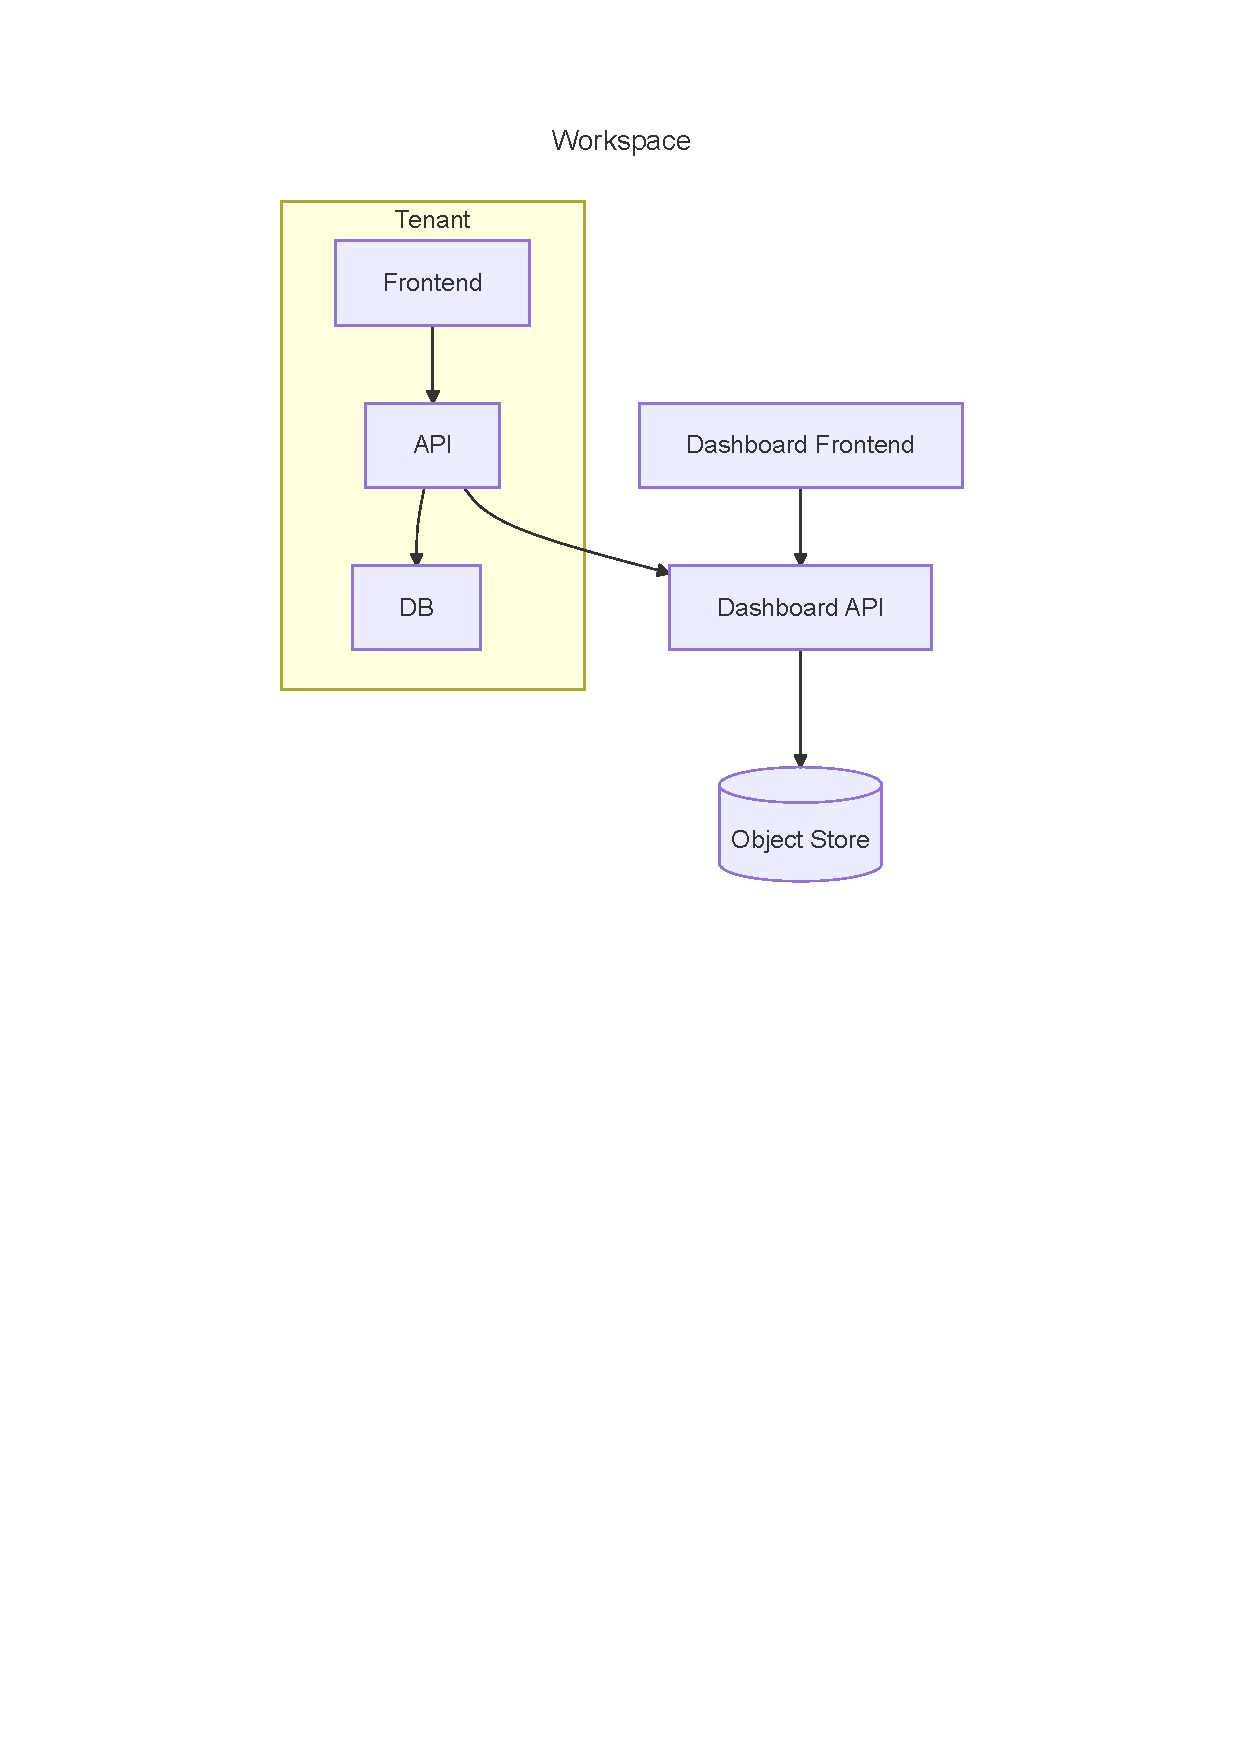
\includegraphics[scale=0.75]{images/WorkspaceArchitecture.pdf}
                    \caption{Overview of the system architecture}\label{fig:system-architecture}
                \end{figure}

            \subsubsection{Rationale for Config Injection Strategy}\label{subsubsec:rationale}
                To balance isolation, simplicity, and edit propagation, configuration delivery
                follows a \textbf{hybrid} approach.
                To enable tenant-specific customization in a secure and maintainable manner, the
                configuration is injected directly into the \gls{api} container during image build
                time using the \gls{docker} \texttt{--build-arg} mechanism.
                This approach ensures that the configuration resides fully within the corresponding
                tenant's workspace post-deployment, thereby preserving strong workspace isolation.
                Moreover, it avoids the operational complexity associated with runtime config
                injection mechanisms and simplifies the tenant lifecycle by keeping all relevant
                data embedded within the container image.\\
                To propagate changes during runtime, a custom versioned \gls{crd} is used.
                The \gls{crd} is created inside the dashboard cluster and bound to the tenant
                cluster using \gls{kcp}.
                This allows for runtime updates without redeploying the entire application while
                preserving strong workspace isolation.
                \\
                Several alternative approaches were considered during the design process.
                Each of them was evaluated based on criteria such as workspace boundary isolation,
                persistence, scalability, operational complexity, and dependency footprint.
                The following list summarizes these alternatives and the primary reasons for their
                exclusion:

                \begin{enumerate}[label={[\arabic*]:},
                    ref=Challenge~\arabic*,
                    leftmargin=*,
                    itemsep=0.6\baselineskip]

                    \item\label{chal:pv}
                        \textit{\gls{pv}}.
                        \glspl{pv} offer cluster-wide storage, but they are bound to the
                        underlying infrastructure and not scoped to individual workspaces.
                        Since tenant data must remain fully isolated within its respective
                        workspace, using a shared \gls{pv} would have violated this design
                        constraint.
                        Furthermore \glspl{pv} would introduce significant operational complexity.
                        
                    \item\label{chal:pvc}
                        \textit{\gls{pvc}}.
                        \glspl{pvc} are workspace-scoped and technically suitable for storing tenant
                        configuration.
                        However, managing their lifecycle dynamically per tenant (including updates
                        and clean-up) would introduce significant operational complexity.

                    \item\label{chal:configMap}
                        \textit{ConfigMap}.
                        A ConfigMap is a lightweight and \gls{k8s} native way to inject
                        configuration, but it has a very constraining size limit (typically 1 MiB)
                        and is not designed for cross-workspace usage.  
                        Since KCP workspaces enforce strict isolation, injecting a ConfigMap from
                        the parent workspace into the tenant workspace would violate boundary
                        constraints, or require custom controllers.  
                        It was primarily not considered a viable long-term option due to its limited
                        support for binary data and poor scalability with growing or media-rich
                        configuration payloads.

                    \item\label{chal:gitRepo}
                        \textit{Git Repository}.
                        Polling or pulling tenant configuration from a Git repository would offer
                        central control and versioning, but would couple each tenant's runtime to an
                        external dependency.
                        It would also require embedding Git credentials or \gls{ssh} keys within the
                        workspace, raising security concerns and operational burden.
                        Furthermore the data does not live inside the tenant violating isolation
                        principles.

                    \item\label{chal:initContainer}
                        \textit{initContainer + emptyDir}.
                        This approach involves using an \texttt{initContainer} to write the config
                        into an \texttt{emptyDir} shared volume before the main \gls{api} container
                        starts.
                        While this ensures data locality, the config is ephemeral and lost on pod
                        restart or rescheduling.
                        Additionally, updates would require a full pod redeployment including
                        controlled init re-execution, adding complexity.

                    \item\label{chal:tenantDB}
                        \textit{Tenant \gls{db}}.
                        Storing the configuration in the tenant database would offer persistence and
                        locality.
                        However access control for the write operations and reaching out to the
                        \gls{db} from the parent workspace are critical pain points.

                    \item\label{chal:redis}
                        \textit{\gls{redis}}.
                        A Redis store within the tenant workspace was considered for fast config
                        access.
                        However, this introduces a full additional service dependency per tenant,
                        which contradicts the goals of lightweight and cost-efficient tenant
                        deployments.
                        Redis also requires persistence management if configuration must survive
                        restarts, therefore adding complexity.

                    \item\label{cahl:centralStore}
                        \textit{Central Document Store}
                        Maintaining a central document store in the root workspace (e.g. MongoDB or
                        MinIO) was ruled out due to isolation concerns.
                        This would require the tenant \gls{api} to reach out beyond its workspace
                        boundary, which is explicitly avoided in the current architecture to enforce
                        strict data sovereignty per tenant.
                \end{enumerate}

                Ultimately, the chosen build-time config injection strategy in combination with the
                \gls{crd} at runtime strikes an effective balance between strong tenant isolation,
                operational simplicity, and runtime performance.
                It also provides a fallback mechanism for configuration changes without requiring
                a full image rebuild.

    \clearpage

            \subsubsection{Data Synchronization and Caching Strategy}\label{syncAndCache}
                As the tenant-\gls{api} is built with its own \textbf{static} \texttt{config.json}
                as shown above \see{subsubsec:rationale}, the resulting caching strategy is
                straightforward.
                At startup the tenant-\gls{api} reads the immutable \texttt{config.json} that is
                baked into the container images \gls{fs}.
                Because the file never changes, while the image is running, the \gls{api} loads its
                content once, materializes the contents \textbf{in memory}, and attaches a single
                long-lived cache entry with a \gls{ttl} of 24~hours.
                A daily \gls{ttl} offers two advantages without introducing the complexity of an
                explicit cache invalidation.
                
                \begin{enumerate}[label={[\arabic*]:},
                    ref=Challenge~\arabic*,
                    leftmargin=*,
                    itemsep=0.6\baselineskip]

                    \item\label{chal:cachePerformance}
                        \textit{Performance}.
                        Subsequent requests bypass \gls{fs} \gls{io} entirely and are served from
                        memory, massively increasing speed and reducing disk pressure under burst
                        traffic.

                    \item\label{chal:cacheResilience}
                        \textit{Resilience and self-healing}.
                        Although the file is static, a bounded \gls{ttl} guarantees that each pod
                        refreshes its configuration once per day, so \textit{\gls{bitrot}} or a
                        silently corrupted memory page cannot persist indefinitely.
                        
                \end{enumerate}

                Because the only legitimate way to alter tenant configuration is to propagate
                changes via the \gls{crd}, a shorter \gls{ttl} or a manual cache-flush \gls{api}
                would add operational complexity without practical benefit.
                Caching the configuration with a long \gls{ttl} therefore strikes the best balance
                between maximal runtime throughput and the minimal housekeeping needed to keep every
                pod's view of configuration fresh and fault-tolerant over time.

            \subsubsection{Workspace Topology and Multi-Tenancy model}\label{subsubsec:workspaceTopology}
                \begin{table}[H]\label{tab:layersOverview}
                    \centering
                    \renewcommand{\arraystretch}{1.25}
                    \setlength{\tabcolsep}{6pt}
                    \begin{tabularx}{\textwidth}{@{} l C{3cm} Y R{2.2cm} @{}}
                        Layer & \gls{kcp} construct & Example resources & Provisioned Amount \\
                        \midrule
                        Parent (control) & Workspace (\texttt{root}) & \texttt{dashboard}, \texttt{dashboard-api} Deployments & 1 (static) \\
                        Tenant (data) & Workspace (\texttt{root:<tenant-id>}) & \texttt{frontend}, \texttt{tenant-api} Deployments, \texttt{\gls{db}}~StatefulSet & 1 per tenant \\
                        \bottomrule
                    \end{tabularx}
                    \caption{Overview of architectural layers}
                \end{table}

                The system architecture is logically divided into two primary layers, a static
                parent workspace and a dynamically provisioned set of tenant workspaces.
                Each layer corresponds to a dedicated \gls{kcp} workspace and fulfills distinct
                responsibilities.
                \\
                The parent workspace acts as the control plane of the system.
                It hosts globally accessible resources such as the Dashboard frontend and the
                \gls{api} responsible for tenant lifecycle management.
                It exists as a single static \texttt{root} workspace and is not scaled horizontally.
                \\
                Each tenant is isolated in its own dedicated workspace (\texttt{root:<tenant-id>})
                created via \gls{kcp}'s Workspace \gls{crd} \gls{api}.
                These tenant workspaces are dynamically provisioned on demand through the
                \texttt{dashboard-\gls{api}}.
                They encapsulate all data and execution logic associated with the tenant, including
                the tenant-specific \gls{api}, frontend, and database state.
                \\
                Tenant workspaces are strictly isolated from each other and from the parent
                workspace.
                All tenant-related resources, including configuration and persistent state, reside
                exclusively within their respective workspaces, maintaining full logical and
                operational isolation.
                \\
                Deleting a workspace recursively tears down all associated Kubernetes resources,
                ensuring complete and automated cleanup without additional control-plane logic.
                \cleardoublepage

            \subsubsection{Tenant Workspace: Data Plane Components}

                \begin{table}[H]\label{tab:tenantComponents}
                    \centering
                    \renewcommand{\arraystretch}{1.5}
                    \begin{tabular}{lp{4cm}P{8cm}}
                        \toprule
                        Component & Scaling & Purpose \\
                        \midrule
                        Frontend (\gls{next}) & \gls{hpa} based on \gls{cpu} and \gls{qps} & Serves static \gls{html} / \gls{js}, does \gls{ssr} for dynamic contents \\
                        \gls{api} (\gls{node}) & \gls{hpa} & Auth-less \gls{rest} endpoints with cache consumed by the \gls{next} app. \\
                        \gls{db} & StatefulSet & Stores ratings \\
                        \bottomrule
                    \end{tabular}
                    \caption{Per Tenant Components}
                \end{table}

                The request flow of the visitor path can be summarized as follows:

                \begin{enumerate}[label={[\arabic*]:},
                    ref=Challenge~\arabic*,
                    leftmargin=*,
                    itemsep=0.6\baselineskip]

                    \item\label{chal:frontend}
                        \textit{Frontend}.
                        The \gls{next} frontend is called.
                    \item\label{chal:tenantApi}
                        \textit{Tenant \gls{api}}.
                        The \gls{next} frontend calls the tenant \gls{api} to get dynamic data.
                        The tenant \gls{api} reads from the cache.

                    \item\label{chal:db}
                        \textit{Data sources}.
                        The tenant \gls{api} periodically renews its cache based of a \gls{ttl}.
                        The dynamic data (reviews) comes from the tenant \gls{db} while the static
                        data (config) comes from the tenant \gls{api}.
                \end{enumerate}

                This ensures, that for all customer interactions on the public website the workload
                remains local to the tenant workspace, thus improving the traceability.

            \subsubsection{Parent Workspace: Control Plane Components}\label{subsubsec:controlPlaneComponents}
                
                \begin{table}[H]\label{tab:parentComponents}
                    \centering
                    \renewcommand{\arraystretch}{1.5}
                    \begin{tabular}{lp{3.5cm}P{8cm}}
                        \toprule
                        Component & Scaling & Purpose \\
                        \midrule
                        Dashboard & \gls{hpa} & Authenticated \gls{ui} for tenant owners; \gls{crud} operations on tenant data \\
                        Parent \gls{api} & \gls{hpa} & validates input and writes \gls{json} \\
                        \bottomrule
                    \end{tabular}
                    \caption{Control Plane Components}
                \end{table}

            \subsubsection{Scalability, Isolation and Security}\label{scalabilityIsolationSecurity}
                The described architecture should be able to provide a high level of scalability,
                isolation and security for the stated use case.
                It should achieve this as follows:

                \begin{enumerate}[label={[\arabic*]:},
                    ref=Challenge~\arabic*,
                    leftmargin=*,
                    itemsep=0.6\baselineskip]

                    \item\label{chal:architectureScalability}
                        \textit{Horizontal Scalability}.
                        Inside the tenant workspace the tenant-\gls{fe} and the tenant-\gls{api} run
                        as stateless deployments.
                        A \gls{hpa} driven by \gls{cpu} utilization and \gls{qps} metrics adds or
                        removes replicas linearly, so throughput increases proportionally with the
                        number of pods \see{tab:perTenantComponents}.
                        Because the \gls{api} keeps no local state, new replicas can be scheduled on
                        any node without coordination, ensuring that burst traffic on popular sites
                        never impacts neighboring tenants.

                    \item\label{chal:architectureIsolation}
                        \textit{Tenant Isolation}.
                        Every customer receives its own dedicated \gls{kcp} workspace at onboarding
                        time.
                        A workspace maps to a private logical cluster stored in an independent
                        \gls{etcd} prefix, so objects created by one tenant are completely invisible
                        to others.
                        All runtime artifacts --- \gls{fe} pods, \gls{api} pods, \gls{db} and even
                        the \texttt{config.json} injected into the \gls{api} --- live exclusively
                        inside that workspace.
                        The \gls{crd} is only bound to the specific tenant workspace.
                        The platform never mounts cross-workspace volumes or reaches out to shared
                        data services.
                        Because there is \textbf{no shared state across workspaces} the design
                        should eliminate noisy-neighbor effects, simplify compliance and guarantee
                        data sovereignty for every tenant.

                    \item\label{chal:architectureSecurity}
                        \textit{Security}.
                        Multi-tenancy is only acceptable if confidentiality and integrity are
                        preserved across tenant boundaries.
                        \autoref{subsubsec:challenges} highlighted, that residual-data exposure,
                        cross-tenant access and side-channel attacks are the primary threats in
                        shared environments.
                        Because every tenant runs inside its \textbf{own} \gls{kcp} workspace,
                        backed by a private \gls{etcd} prefix, objects created in one workspace are
                        completely invisible to others, including non-namespaced objects like
                        \glspl{crd} \parencite{kcpWorkspaces}.
                        This hard logical boundary, combined with the absence of any shared state
                        outside the workspace allows for:
                        \\
                        \textbf{Data confidentiality}, as data resides inside the tenant,
                        eliminating residual-data exposure vectors.
                        \\
                        \textbf{Privilege containment}, as workspace-local \gls{rbac} rules grant
                        only verbs needed to operate intra-workspace resources and there are no
                        cluster-wide roles, blocking lateral movement and privilege-escalation
                        attempts.
                        \\
                        \textbf{Secure storage}, as only the tenant-\gls{api} has write access on
                        the tenant-\gls{db}.
                        \\
                        By confining a potential attacker to the compromised workspace, the
                        architecture should neutralize the multi-tenant security risks identified
                        earlier while still reaping the economic benefits of sharing the underlying
                        platform.
                        
                \end{enumerate}

                Collectively the security measures have to fulfill \hyperlink{NF-07}{nf7}. \\
                \gls{hpa} in Kubernetes can react to any metric that the control plane exposes
                through resource or custom-metrics \glspl{api}.
                For a request-driven \textit{express} service, such as the tenant-\gls{api} the most
                accurate signal would be \textbf{\gls{qps}} at the ingress of each pod, because it
                tracks the real work performed and is immune to the noise that \gls{cpu}-bound
                metrics introduce when background jobs or garbage collection dominate a sample
                window.
                Nevertheless, the implementation in its prototypical nature should deliberately rely
                on the built-in \textbf{\gls{cpu} utilization metric} alone, contrary to the
                architectural best practices.
                The choice is pragmatic rather than idealistic.
                Instrumenting per-pod \gls{qps} would require an extra metrics pipeline or at
                minimum a side-car that counts requests, a Prometheus deployment to scrape the
                counter, and a Prometheus adapter (or custom-metrics server) so the \gls{hpa}
                controller can consume the data.
                Each of those moving parts introduces significant configuration surface, security
                considerations, and potential failure modes that distract from the core objective of
                this thesis: to validate multi-tenant isolation and deployment strategies, not to
                engineer a production-grade observability stack.
                \gls{cpu} metrics, by contrast, are available out of the box from the kubelet and
                require only two declarative lines in the \gls{hpa} manifest.
                \\
                Using \gls{cpu} as the scaling trigger therefore keeps the infrastructure
                lightweight, repeatable, and easy to grasp while still demonstrating that the
                platform can elastically adjust capacity under load.
                In a real-world \gls{saas} environment the \gls{hpa} spec could be refined to a
                compound metric using \gls{qps} latency percentiles, or custom business \glspl{kpi}
                \glsadd{kpi@gls}, but for a prototype aimed at architectural proof of concept, the
                built-in metric is \enquote{good enough} and avoids adding too much complexity out
                of the thesis scope.
                
        \clearpage

        \subsection{Automated Deployment Strategies}\label{subsec:deploymentStrategies}
            Platform success depends on a deployment workflow that is fully automated, repeatable,
            and invisible to tenants.
            The design therefore distinguishes between the \textbf{first-time (initial) deployment}
            of a tenant workspace and the \textbf{continuous update policy} that keeps thousands of
            workspaces on a single, uniform release without interrupting production traffic.

            \FloatBarrier
            \subsubsection{Initial Tenant Deployment Pipeline}\label{subsubsec:initialDeeployment}
                When a new customer completes the on-boarding flow \hyperlink{f5}{F-05}, the
                Dashboard-\gls{api} running in the root workspace emits a custom resource
                (\texttt{TenantDeploymentRequest}) that seeds a GitOps pipeline.
                The pipeline is implemented as a set of \textit{\gls{tekton}} tasks that run
                directly under the control of the Dashboard-\gls{api}, therefore no separate
                \textit{\gls{argocd}} controller is required.

                \begin{figure}[tbp]
                    \centering
                    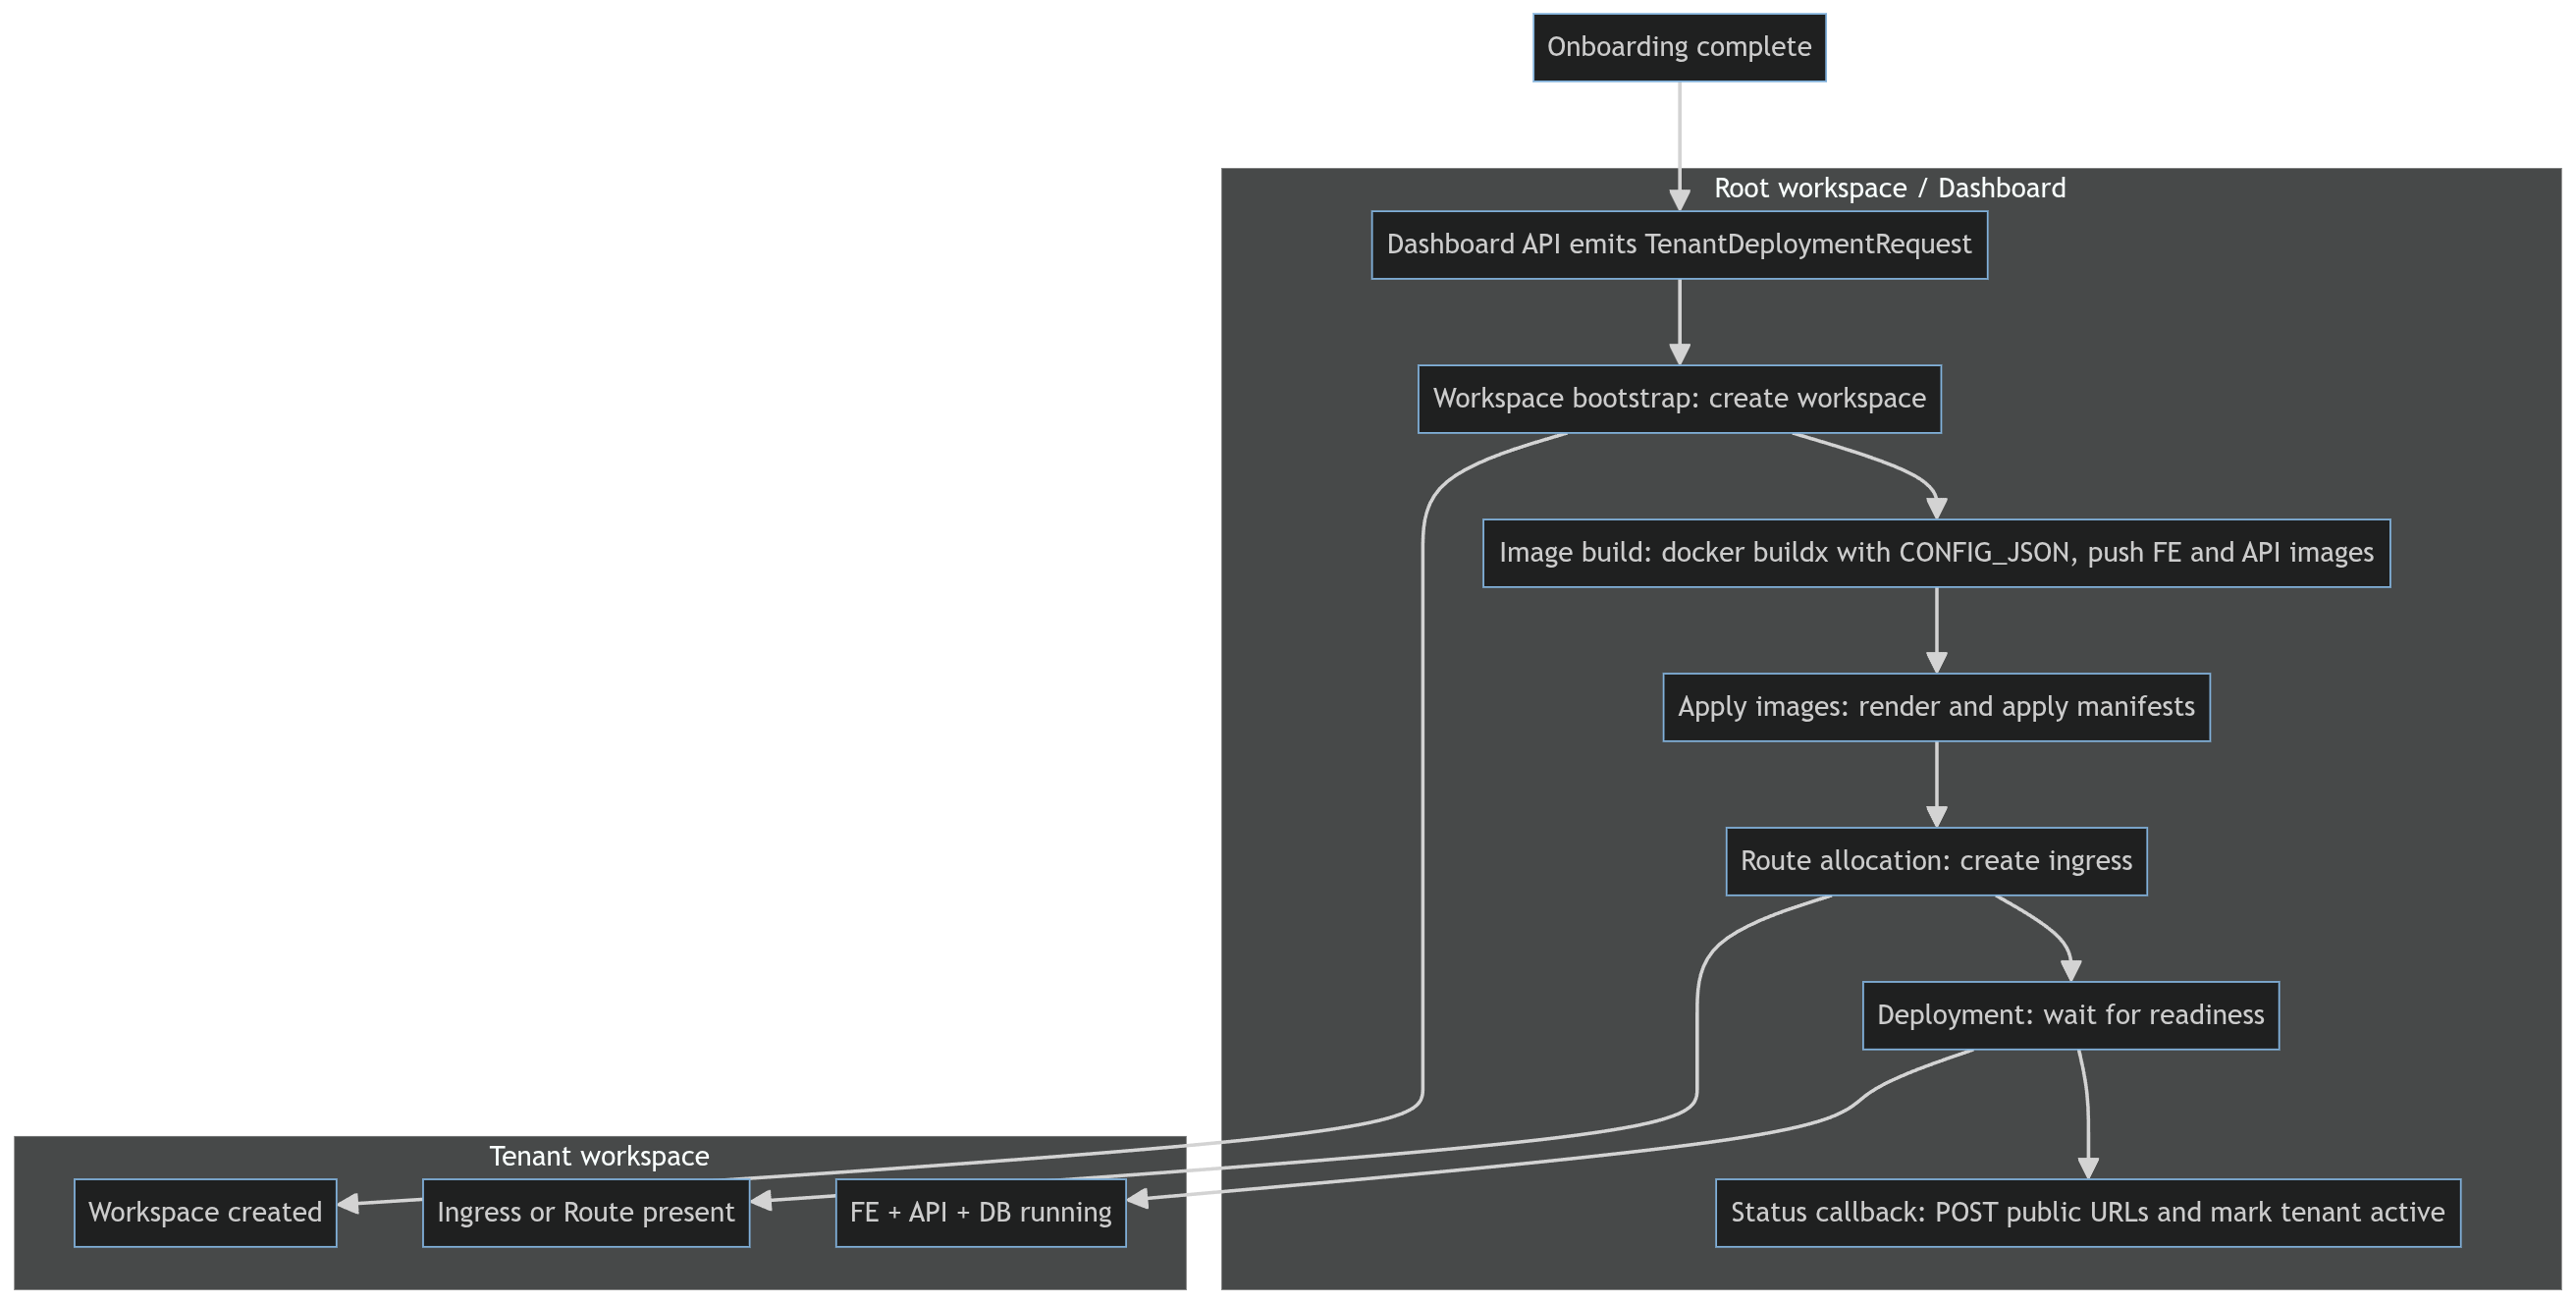
\includegraphics[width=\textwidth]{images/pipeline.png}
                    \caption{Initial tenant deployment pipeline}\label{fig:initial-deployment-pipeline}
                \end{figure}

                \begin{enumerate}[label={[\arabic*]:},
                    ref=Challenge~\arabic*,
                    leftmargin=*,
                    itemsep=0.6\baselineskip]

                    \item\label{chal:bootstrap}
                        \textit{Workspace bootstrap}.  
                        A controller watching for \texttt{TenantDeploymentRequest} objects
                        calls the \gls{kcp} \gls{api} to create a dedicated workspace
                        \texttt{root:\textless{}tenant-id\textgreater{}} and assigns only the
                        minimal \gls{rbac} roles required by the tenant components.

                    \item\label{chal:imageBuild}
                        \textit{Image build}.
                        A build task invokes \texttt{docker buildx} with
                        \texttt{--build-arg CONFIG\_JSON} to inject the tenant-specific
                        configuration into the \gls{api} image layer
                        (cf.~\autoref{subsubsec:rationale}).  
                        The resulting \gls{api} and \gls{fe} images are pushed to the internal
                        registry and tagged
                        \texttt{:\textless{}tenant-id\textgreater{}-\textless{}git-sha\textgreater{}}.

                    \item\label{chal:manifestRendering}
                        \textit{Manifest rendering}.
                        Helm/Kustomize templates are parameterized with the tenant ID, image
                        tags and a computed \texttt{ROUTE\_BASE} and rendered to plain \gls{yaml}.

                    \item\label{chal:routeAllocation}
                        \textit{Route allocation}.
                        The pipeline creates an \texttt{Ingress} (nginx) or \texttt{Route}
                        (OpenShift) inside the tenant workspace.
                        A wildcard \gls{dns} entry (\texttt{*.example.com}) avoids central \gls{dns}
                        updates and keeps certificates simple.

                    \item\label{chal:applyManifests}
                        \textit{Deployment}.  
                        A Helm \texttt{upgrade --install} task applies the rendered manifests
                        in the tenant workspace, rolling out the \gls{fe}, \gls{api} and
                        backing \gls{db}.  
                        Readiness probes ensure the pipeline blocks until all Pods are ready.

                    \item\label{chal:callback}
                        \textit{Status callback}.  
                        Once every component is healthy, a final task POSTs the public \glspl{url}
                        and the image \gls{sha} back to the Dashboard-\gls{api}, which in turn marks
                        the tenant as \enquote{active} for subsequent logins.
                \end{enumerate}

                By chaining these \gls{tekton} tasks the platform turns the single
                \texttt{TenantDeploymentRequest} event into a fully-isolated, routable tenant
                environment in one pass.
                Every artefact is generated from code that lives in Git, every cluster mutation is
                scoped to the tenant workspace, and every build is automatically signed by
                \gls{tekton}~Chains.
                Consequently the pipeline satisfies all functional requirements while
                remaining short enough to version-control next to the product source and easy to
                extend with additional steps (e.g.\ quota enforcement or cost metering) as the
                service matures.

            \FloatBarrier
            \subsubsection{Continuous Deployment}\label{subsubsec:continuousDeployment}
                After the initial hand-off the platform must react to two kinds of change without
                operator intervention:

                \begin{enumerate}[label={[\arabic*]:},
                    ref=Challenge~\arabic*,
                    leftmargin=*,
                    itemsep=0.6\baselineskip]

                    \item\label{chal:cdCode}
                        \textit{Source-code updates}.
                        A merge on the main branch of either the tenant \gls{fe} or the tenant
                        \gls{api} Git repository emits a signed GitHub Webhook.
                        This triggers a pipeline that builds the updated image and rolls it out.
                        
                    \item\label{chal:cdData}
                        \textit{Content-driven updates (single tenant rebuild)}.
                        When business users change dynamic catalogue data or feature flags, the
                        dashboard \gls{api} issues a \texttt{TenantReconfigureRequest} object
                        that carries the new \texttt{config.json} payload.  
                        A dedicated \gls{tekton} pipeline in that tenant's workspace creates
                        the \gls{crd} carrying the \gls{json} payload and binds it to the tenant
                        workspace.
                        Following this a local \gls{helm} upgrade of the tenant \gls{api} is
                        performed, while the \gls{fe} and \gls{db} remain untouched.

                \end{enumerate}

                \subsubsection{Zero-Downtime Rollout}\label{subsubsec:zeroDowntime}

                    The continuous-deployment pipeline should deploy the updated version of the
                    tenant code with zero downtime for customers while ensuring stability.
                    This can be achieved through a \textit{canary deployment}.
                    A canary deployment is a type of blue-green deployment strategy
                    \parencite[pp.~33--34]{awsOverviewDeploymentOptions}.
                    Blue-green deployments are a common deployment strategy to ensure zero downtime.
                    In a blue-green deployment the currently running application (blue) runs
                    alongside the newly deployed, updated application (green)
                    \parencite[pp.~32--33]{awsOverviewDeploymentOptions}[pp.~176--178]{davis2019}.
                    This allows for testing the green version in production, while still having the
                    blue version live to handle production traffic
                    \parencite[pp.~176--178]{davis2019}.
                    With a canary deployment, the cut-over from blue to green is performed
                    gradually \parencite[pp.~33--34]{awsOverviewDeploymentOptions}.
                    A small percentage of traffic is first routed to the green application,
                    the \textit{canary-group}, so that its real-world behavior can be observed under
                    production load \parencite[pp.~33--34]{awsOverviewDeploymentOptions}.
                    If no regressions are detected, the remaining traffic is shifted either in one
                    further step or through a series of linear increments until 100 \% of users are
                    served by the green version
                    \parencite[pp.~33--34]{awsOverviewDeploymentOptions}.
                    Because the blue environment remains intact throughout the process, any anomaly
                    can be mitigated instantly by redirecting requests back to it, thereby
                    minimizing blast radius while still achieving zero downtime for customers
                    \parencite[pp.~33--34]{awsOverviewDeploymentOptions}.
                    \\
                    Broken down step by step, the pipeline should act as follows:
                    
                    \begin{enumerate}[label={[\arabic*]:},
                        ref=Challenge~\arabic*,
                        leftmargin=*,
                        itemsep=0.6\baselineskip]

                        \item\label{chal:readinessProbe}
                            \textit{Readiness probe}.
                            Verifies readiness probes and functional smoke-tests on the green Pods.

                        \item\label{chal:shiftTraffic}.
                            \textit{Shift traffic}.
                            Shifts traffic incrementally by patching the weight on the tenant's
                            ingress.

                        \item\label{chal:canaryWindow}
                            \textit{Canary window}.
                            Aborts and rewinds the weight if any \gls{slo} breach or error-budget
                            drain is detected during the canary window.
                        
                        \item\label{chal:deletion}
                            \textit{Deletion}.
                            Deletes the blue deployment only after 100 \% of requests have
                            successfully moved to green.

                    \end{enumerate}

            \clearpage

        \subsection{Choice of Technologies}\label{subsec:technologies}
            The platform architecture leverages modern, well-supported technologies that align with
            the core design principles of modularity, performance, and isolation with the addition
            of the promising bleeding edge \gls{kcp} project.
            Each major component is built using tools selected for their suitability in a
            cloud-native, tenant-isolated \gls{saas} environment.

            \begin{enumerate}[label={[\arabic*]:},
                ref=Challenge~\arabic*,
                leftmargin=*,
                itemsep=0.6\baselineskip]
                \item\label{chal:dashboardFE}
                    \textit{Dashboard \gls{fe}}.
                    The central Dashboard is implemented using \texttt{\gls{next}}.
                    Its file-based routing, support for both static and server-side rendering, and
                    seamless integration with TypeScript make it a suitable choice for building a
                    modular and responsive frontend.
                    Reusability and developer ergonomics were key factors in this decision.

                \item\label{chal:tenantFE}
                    \textit{Tenant \gls{fe}}.
                    Each tenant is provisioned with a separate frontend instance based on a shared
                    \texttt{\gls{next}} template.
                    This enables customization at the workspace level while maintaining consistent
                    structure and behavior.
                    \gls{next} also allows efficient static generation of tenant-specific content
                    during build time.
                    To further streamline provisioning, a pre-defined set of layout and component
                    \textit{skeletons} is embedded in the template repository.  
                    These skeletons provide a consistent structure for common views, while still
                    allowing per-tenant extension and branding.

                \item\label{chal:dashboardAPI}
                    \textit{Dashboard \gls{api}}.
                    The control plane's \gls{api} is built using \texttt{\gls{node}} and
                    \texttt{\gls{express}}, providing a lightweight, fast, and \gls{json}-native web
                    service environment.
                    It integrates a volatile \texttt{node-cache} layer for storing configuration
                    artifacts during tenant provisioning, minimizing external dependencies.

                \item\label{chal:tenantAPI}
                    \textit{Tenant \gls{api}}.
                    Each tenant workspace contains its own
                    \texttt{\gls{node}}~+~\texttt{\gls{express}} \gls{api} instance.
                    This ensures strict separation of runtime logic and supports injection of static
                    configuration at image build time.
                    The framework's flexibility and ecosystem make it well-suited for containerized
                    multi-tenant deployment.

                \item\label{chal:tempConfigStore}
                    \textit{Temporary Config Store}.
                    During tenant creation, configuration files are temporarily stored on the
                    Dashboard \gls{api}'s local filesystem.
                    These files are injected into the tenant image using Docker's
                    \texttt{--build-arg} and \texttt{COPY} mechanisms for initialization or
                    injected into the tenant workspace at runtime via a \gls{crd}.
                    This avoids cross-workspace communication and external storage dependencies.
                    This enables runtime updates and a safe, clean way to provide the config to the
                    tenant cluster for both initialization and runtime updates.

                \item\label{chal:tenantDB2}
                    \textit{Tenant \gls{db}}.
                    The tenants database layer is provided by \texttt{Citus}, a horizontally
                    scalable extension of PostgreSQL.\@
                    Citus allows sharded, isolated storage of tenant data and supports scaling out
                    as load increases.
                    Its compatibility with PostgreSQL clients simplifies development and
                    integration.

            \end{enumerate}

            This technology selection provides a robust foundation for implementing the desired
            multi-tenant \gls{saas} architecture while keeping the operational footprint minimal and
            the development process maintainable.
            Furthermore it aims to live inside the \gls{ts} ecosystem, simplifying the development
            process.

    \clearpage

    \section{Prototypical Implementation}\label{sec:prototype}

        \subsection{Purpose and Reading Guide}\label{subsec:purposeAndReadingGuide}
            This chapter explains how the architecture described in
            \autoref{subsec:architectureDesign} was turned into a working prototype.
            It documents what was implemented, how each piece maps back to the design, and why
            specific trade-offs were made.
            The \gls{dod} for the prototype was one end-to-end tenant lifecycle as described in
            the user journey \autoref{subsubsec:userJourney} with functional backends and frontends,
            container images, \gls{k8s@gls} manifests and automation scripts.

            \paragraph{How to read this chapter.}\label{par:howToReadThisChapter}
                First, the path from design to code is outlined, followed by a description of the
                environment to ensure a reproducible build.
                Subsequent sections cover templates and schemas, the four core services
                (tenant \gls{fe}/\gls{be}, dashboard \gls{fe}/\gls{be}), and cross-cutting concerns
                (configuration via \gls{crd} and \gls{api}Binding, security/\gls{rbac}, networking, 
                resource management).
                The chapter then turns to infrastructure and deployment, challenges encountered,
                deviations from the design, and limitations.
                Where applicable, sections provide links to the appendix sections that contain the
                corresponding code snippets.

            \paragraph{Where the code lives.}\label{par:whereTheCodeLives}
                All code artifacts are reproduced in the code appendices: B-G contain the directory
                structure, key files, and selected code snippets for the core applications, the
                configuration schema, and the infrastructure.
                Appendix~A gives a quick map of repositories and their contents.

            \paragraph{Conventions.}\label{par:conventions}
                File and directory names appear in \texttt{monospace}.
                Source snippets are shown as \emph{listings} with line numbers.
                Long listings may span multiple pages.
                Figures are used for structure (e.g., directory trees).

    \clearpage

        \subsection{From Design to Code}\label{subsec:fromDesignToCode}
            This subsection traces the concrete path from the architectural design to a working
            system.
            The implementation was structured as a sequence of vertical slices that each deliver
            \gls{e2e} functionality, while continuously aligning with the multi-tenant architecture.

            \paragraph{Repository and scaffold setup}
                Separate repositories were created for each bounded component: tenant \gls{fe},
                tenant \gls{be}, dashboard \gls{fe}, dashboard \gls{be}, the configuration schema,
                and the infrastructure.
                An overview and links to the repositories are listed in
                Appendix~\ref{app:repos-overview}.
                The concrete code is documented in
                Appendices~\ref{app:tenantfe},~\ref{app:tenantbe},~\ref{app:dashboardfe},~\ref{app:dashboardbe},~\ref{app:configschema}, and~\ref{app:infra}.
                Each service was initialized with a minimal, runnable skeleton including a
                dockerfile.

        \subsection{Environment and Reproducibility}\label{subsec:environmentAndReproducibility}
            The prototype is packaged to be rebuilt and executed from a clean developer machine with
            minimal manual steps.
            The \textit{Infra} repository (Appendix~\ref{app:infra}) serves as the orchestrator:
            it vendors \gls{k8s@gls} manifests, pins tool and image versions, and provides
            idempotent scripts for bootstrapping, building, and deploying all services.

            \paragraph{Baseline toolchain}
                A container-first setup is used to maximize reproducibility.
                Services are build into \gls{docker} images with explicit base-image tags.
                Clusters are provisioned using \textit{kind}.
                Deployment is performed via checked in manifests.
                Required \gls{cli} tools are installed and partly pinned by helper scripts.

            \paragraph{Determinism safeguards}
                Reproducibility is reinforced by:
                \begin{enumerate}[label={[\arabic*]:},
                    ref=Challenge~\arabic*,
                    leftmargin=*,
                    itemsep=0.6\baselineskip]

                    \item\label{chal:pinned}
                        \textit{Tags and versions}.
                        Explicit image tags and pinned tool versions.
                        
                    \item\label{chal:manifests}
                        \textit{Manifests}.
                        Declarative manifests committed to \gls{vcs}.

                    \item\label{chal:scripting}
                        \textit{Scripting}.
                        Shell scripts that automate the build and deployment process.
                        Most are idempotent and can be run multiple times without side effects.

                \end{enumerate}

    \clearpage

        \subsection{Templates and Schemas}\label{subsec:templatesAndSchemas}
            This section introduces the code templates used to standardize the \gls{fe} and \gls{be}
            repos in terms of project configuration.
            The goal is to minimize boilerplate decisions.
            Furthermore it introduces the configuration schema used to validate the tenant
            configuration and provide the data type across services.

            \subsubsection{Frontend Template}\label{subsubsec:frontendTemplate}
                The frontend template provides a Next.js / TypeScript boilerplate including an
                \texttt{.editorconfig}, a \texttt{tsconfig.json}.
                Furthermore it includes code quality tooling configuration for ESLint and Prettier
                as well as a boilerplate multi-stage Dockerfile.
                Both frontends, the tenant \gls{fe} and the dashboard \gls{fe}, are based on this
                template repository.\\
                Due to its minor relevance for the thesis, the template repository contents are not
                reproduced in the appendix.

            \subsubsection{Backend Template}\label{subsubsec:backendTemplate}
                The backend template offers a TypeScript / Node (Express) baseline with the same
                tooling and conventions as the frontend to reduce cognitive switching and friction.
                It includes a \texttt{tsconfig.json}, a \texttt{.editorconfig}, ESLint and Prettier,
                and a boilerplate multi-stage Dockerfile.\\
                Due to the again minor relevance for the thesis, the template repository contents
                are not reproduced in the appendix.

            \subsubsection{Configuration Schema}\label{subsubsec:configSchema}
                A central \texttt{zod} schema is used to validate and version the tenant
                configuration.
                It can be imported by all services to ensure consistent data types and validation.
                The schema enables runtime validation with distinct error messages at service 
                boundaries as well as a TypeScript type definition for type safety.
                It was published as a \texttt{npm} package to allow for easy imports and
                maintainability across all core services.\\
                The same structure underlies the versioned \gls{crd} used to make the configuration
                available in the tenant workspace.
                The schema and its unit tests are shown in Appendix~\ref{app:configschema}.

    \clearpage

        \subsection{Core Components}\label{subsec:coreComponents}
            This section describes the four runtime services at a high level and their
            responsibilities within the architecture.
            Each of the sections below states the component's role and boundaries, its key
            dependencies and the contracts it exposes.
            Cross-cutting topics such as configuration, propagation with \glspl{crd} and
            APIBindings, \gls{rbac}, networking and port mappings are treated separately
            in~\ref{subsec:crossCuttingConcerns} and~\ref{subsec:challengesAndBugs}.

            \subsubsection{Tenant Frontend}\label{subsubsec:tenantFrontend}
                The tenant frontend is a small Next.js (App Router) site that renders the tenant's
                public page from the shared configuration and exposes a deliberate failure trigger
                for the tenant backend for chaos testing.\\
                The \texttt{layout.tsx} file fetches the tenant configuration from the tenant
                backend's \texttt{/config} endpoint and passes it to the page component,
                revalidating every ten minutes. 
                It is depicted in~\autoref{lst:tenantfe-layout}.\\
                The result is stored in a react context so the root page can access it without
                fetching --- enabling \gls{ssr}.
                The context provider is depicted in~\autoref{lst:tenantfe-configprovider}.\\
                The root page uses this context and renders company details, proposition,
                products etc.\@as shown in~\autoref{lst:tenantfe-page}.\\
                Using \gls{isr} ensures that changes to the tenant's config become visible within
                at most ten minutes without a full rebuild, while still serving static \gls{html}
                between refreshes.\\
                A \enquote{crash} button issues a request to the tenant \gls{api}'s \texttt{/crash}
                endpoint to intentionally terminate that service.
                This allows testing the backends recovery behavior.\\
                The Dockerfile accepts the endpoint \glspl{url} as build arguments.
                These are baked into the frontend as environment variables at build time.
                It is shown under~\autoref{lst:tenantfe-dockerfile}.

            \subsubsection{Tenant API}\label{subsubsec:tenantAPI}
                A minimal Node / Express service that exposes exactly two endpoints and serves as
                the tenant's backend.\\
                \texttt{/config} returns the tenant's configuration as a \gls{json} object.\\
                \texttt{/crash} deliberately terminates the service using
                \texttt{process.exit(1)} to support failure-injection experiments for evaluation.\\% chktex 36
                The service reads a single \gls{json} file baked into the image at build time and
                serves it via \texttt{/config}.
                The intended design was to watch and fetch the latest config from the \gls{crd}
                during runtime, so updates would flow through without a rebuild.
                That integration did not work and is discussed in~\autoref{subsec:challengesAndBugs}.
                Until then, the backend operates on the immutable file included during the image
                build.
                The \texttt{server.ts} is shown under~\autoref{lst:tenantbe-server}.\\
                The dockerfile accepts a \texttt{CONFIG\_PATH} as build argument and copies the
                referenced file into the image to make it available for the service.
                This keeps the container self-contained.
                The dockerfile is shown under~\autoref{lst:tenantbe-dockerfile}.

            \subsubsection{Dashboard Frontend}\label{subsubsec:dashboardFrontend}
                A small Next.js application that provides a minimal login and a tenant-configuration
                form.\\
                The login page accepts a username (no password for simplicity during prototyping)
                and uses a session cookie to keep track of the username.
                This is a placeholder for actual authentication and just implemented to allow
                associating a username with a tenant cluster later on.
                The authentication logic is provided and handled by the login page, depicted
                at~\autoref{lst:dashboardfe-login-page}, the login form, depicted
                at~\autoref{lst:dashboardfe-login-form}, the login action, depicted
                at~\autoref{lst:dashboardfe-login-action} and the auth lib, depicted
                at~\autoref{lst:dashboardfe-auth-lib}.\\
                The root page routes to the login page if no session cookie is present.
                Otherwise it renders the form to create a new tenant or modify an existing one
                (not part of the prototype due to issues discussed
                in~\autoref{subsec:challengesAndBugs}).
                The form is provided by the \texttt{ConfigForm} component, depicted
                at~\autoref{lst:dashboardfe-config-form}.
                It uses the zod schema to safely parse and validate the input and dynamically
                adds input fields to add more products.
                On success, the form data is posted to the dashboard backend as \gls{json}.\\
                The dockerfile accepts the dashboard backend's \texttt{CONFIG\_ENDPOINT} as build
                argument and sets it as an environment variable in the container.
                The dockerfile is shown under~\autoref{lst:dashboardfe-dockerfile}.

            \subsubsection{Dashboard API}\label{subsubsec:dashboardAPI}
                A lightweight Node / Express service that accepts tenant configurations, validates
                them against the zod schema, and was supposed to coordinate lifecycle events for
                the tenant cluster (creation and \gls{crd} updates).\\
                The service exposes a single \texttt{/config} endpoint that accepts a \gls{json}
                payload in a \texttt{POST} request and validates it against the zod schema.
                It reads the tenant username from the session cookie in the request header.
                Furthermore it persists the validated configuration as a file under
                \texttt{data/\$\{user\}/config.json} to allow for later retrieval and usage in the
                tenant lifecycle.
                The \texttt{server.ts} is shown under~\autoref{lst:dashboardbe-server}.\\
                The service also maintains a redis cache to associate usernames with tenant cluster
                \glspl{ip}.
                The redis logic is shown under~\autoref{lst:dashboardbe-redis}.\\
                The dockerfile does not need any build arguments in this case.
                It is shown under~\autoref{lst:dashboardbe-dockerfile}.\\
                The integration with the tenant lifecycle could not be implemented due to issues
                discussed in~\autoref{subsec:challengesAndBugs}.\\
                The service is stateless aside from the ephemeral file drop and the redis lookup
                table.
                Authentication is deliberately minimal to avoid out-of-scope complexity.
                Production hardening is discussed in~\autoref{subsec:limitationsAndRisks}.

        \subsection{Cross-cutting Concerns}\label{subsec:crossCuttingConcerns}
            A single configuration contract (\autoref{app:configschema}) governs both build-time
            creation and runtime use.
            In the prototype, the dashboard \gls{api} validates configs and writes a versioned file
            used as build context for tenant images (\autoref{app:dashboardbe}).
            The intended runtime path, publishing the same structure as a versioned \gls{crd} and
            importing it via \emph{APIBinding} during runtime, is defined
            under~\autoref{lst:create-tenant-crd}.
            Limitations and the resulting fallback possibilities are discussed
            in~\autoref{subsec:challengesAndBugs}.\\
            External access terminates at the dashboard ingress (\autoref{lst:dashboard-ingress})
            however the ingress controller is not fully implemented in the prototype due to
            complexities discussed in~\autoref{subsec:challengesAndBugs}.
            Tenant services are discovered via the dashboard's redis lookup.
            \gls{cors} is restricted to the dashboard origin due to limitations discussed
            in~\autoref{subsec:challengesAndBugs}.
            Traffic and dependencies between tenant and dashboard clusters are avoided by using
            file-based build injection and \glspl{crd} rather than direct calls across clusters
            to achieve isolation.\\
            Validation failures are provided by zod.
            In the case of an \gls{crd} update being unavailable the system degrades to the last
            valid configuration.\\
            All services accept their dependencies via env as build args.

        \subsection{Infrastructure and Deployment}\label{subsec:infrastructureAndDeployment}
            The whole infrastructure is scripted to produce a repeatable demo environment following
            the \texttt{README} file in the \textit{Infra} repository.
            Most util scripts are idempotent and can be run multiple times without side effects.
            The entry point is the \texttt{create-dashboard-workspace.sh} script
            (depicted under~\autoref{lst:create-dashboard-workspace}) creating a \gls{kcp}-\gls{tmc}
            workspace, the dashboard cluster and the deployments for the dashboard \gls{fe} and
            \gls{be}.
            The rationale for using \gls{tmc} is discussed in~\autoref{subsubsec:challengesKCPTMC}.
            All scripts and manifests are listed in~\autoref{app:infra}.\\
            Tooling and cluster prerequisites are prepared by multiple scripts in the \textit{Infra}
            repository ensuring a reproducible environment.\\
            The layout is described in~\autoref{subsec:infra-layout} and the simplified deployment
            workflow is shown in~\autoref{subsec:infra-workflow}.\\
            Service images are built using parametrized scripts as well to ease the process of
            building and deploying the services.\\
            On success the dashboard cluster is ready and the frontend is available at
            \texttt{dashboard.local:8080}.

        \subsection{Challenges, Bugs and Fixes}\label{subsec:challengesAndBugs}
            The prototype spans several layers (Next.js/Express services, container builds,
            \gls{k8s@gls} on \gls{kind}, \gls{kcp}-\gls{tmc} workspaces, and configuration via
            \gls{crd} and \gls{api}Binding).
            Along this path a mix of non-obvious defaults, complexities, version drift and
            underspecified behaviors surfaced.
            This section documents the most consequential issues, why they occurred, how they were
            detected, and the remedies or workaround applied.
            Items are grouped by theme and point to the relevant code in the appendix where
            applicable.
            Where problems remain partially resolved, the residual risks and alternatives are stated
            to inform the evaluation and future work.

            \subsubsection{CORS}\label{subsubsec:challengesCORS}
                Browser backend calls failed with \gls{cors} errors (blocked preflight
                \texttt{OPTIONS} and mismatched \texttt{Origin}).
                The underlying cause was a divergence of hosts and ports between frontend
                \glspl{url} and backend services.
                Attempts to \enquote{open up} \gls{cors} on the backends and to normalize hosts via
                ingress (as described in~\autoref{subsubsec:ingress}) still left inconsistent
                origins during local \gls{kind} testing (multiple ports, per service hostnames),
                so the browser refused the cross-origin requests.\\
                The effective workaround was to route traffic through server-side Next.js handlers
                under \texttt{/api}, so the browser sees a same-origin request and the \gls{fe}
                service then proxies to the \gls{be}.
                This avoids the browsers \gls{cors} checks entirely.
                The proxy preserves method, headers, and body, forwards response status and headers,
                and reads the backend base \gls{url} from an environment variable set at build and
                run time.\\
                The proxy handlers can be found in the appendix
                under~\autoref{lst:tenantfe-config-route},~\autoref{lst:tenantfe-crash-route}
                and~\autoref{lst:dashboardfe-api-config}.\\
                This pattern centralizes auth/cookies and simplifies local development, but it hides
                the browser's true origin from the backend, so any future direct browser to backend
                path must reintroduce strict \gls{cors} and a stable host schema via a gateway or
                ingress and possibly \gls{dns}.
                Once the cluster ingress is finalized, the \gls{cors} proxy can be removed or
                kept as a fallback for local development.

            \subsubsection{Ingress}\label{subsubsec:ingress}
                Declaring an nginx ingress in \gls{k8s@gls} is straightforward
                (cf.~\autoref{lst:dashboard-ingress} and~\autoref{lst:tenant-ingress}).
                The difficulty arose only on a Linux developer machine.
                A typical ingress controller expects to serve on the standard \gls{http} and
                \gls{https} ports \texttt{80} and \texttt{443}, which competes with existing services
                and requires elevated privileges and system tweaks.
                In practice, this turned local setup into \gls{os} plumbing rather than application
                work, straying from the thesis scope.\\
                Introducing MetalLB to gain \texttt{LoadBalancer} services on bare metal was
                discarded due to additional network configuration, \gls{ip} range management and
                operational overhead not central to the thesis.\\
                Given these trade-offs, an ingress on standard ports was deferred for the local
                development.
                The system instead relies on the server-side proxy pattern described
                in~\autoref{subsubsec:challengesCORS} for direct component to component calls.
                The browser still uses the ingress to access the frontends combined with custom
                hostnames in \texttt{/etc/hosts}.
                This keeps the development path simple and reproducible.
                In managed layouts (\gls{eks}, \gls{gke}, \gls{aks}), the intended production
                layout becomes trivial to enable without host-level changes.

            \subsubsection{End-to-End Port Mapping}\label{subsubsec:e2eportmapping}
                Accessing services via \texttt{NodePort} surfaced several mismatches across the
                chain \emph{application $\rightarrow$ container $\rightarrow$ service $\rightarrow$
                cluster-exposed port}.
                The application listened on one port, the container image and deployment declared
                another (\texttt{containerPort}), while the \texttt{Service} used a conflicting
                \texttt{targetPort}/\texttt{port}, and the public \texttt{nodePort} finally exposed
                yet another value.
                The result was traffic black-holing that looked like \gls{cors} or network errors on
                the surface.
                Relevant manifests are listed in~\autoref{app:infra}.\\
                A dedicated \emph{netshoot} pod (\autoref{lst:debug-pod-manifest}) was introduced to
                probe connectivity from inside the cluster.
                This quickly distinguished in-cluster routing issues from host access problems and
                revealed which hop in the mapping was incorrect.\\
                The mapping was normalized to the working version in~\autoref{app:infra}.
                The debug container manifest was deliberately kept in the thesis, because it
                outlines a easy to deploy best practice for debugging network issues in
                \gls{k8s@gls}.

            \subsubsection{Hostnames}\label{subsubsec:hostnames}
                Consistent browser access to cluster services is achieved by mapping friendly
                hostnames (e.g., \texttt{dashboard.local}) to a chosen \gls{ip} via
                \texttt{/etc/hosts}.
                Two small idempotent helpers implement this
                (\autoref{lst:add-to-hosts} and~\autoref{lst:cleanup-hosts}).
                This approach was aimed at easing local development and testing without having to
                look up \glspl{ip} or ports permanently.\\
                Therefore it is deliberately left in the thesis as a reproducible approach, that
                turned out to be useful for local development.

            \subsubsection{KCP-TMC}\label{subsubsec:challengesKCPTMC}
                The initial plan relied on \emph{gls{kcp}} to provision clusters in workspaces.
                However a breaking change between \gls{kcp} \texttt{v0.19} and \texttt{v0.20}
                invalidated that approach.
                The change was made in 2023, however the breaking change was documented only in
                the changelogs and the \gls{kcp} slack channel.
                The stack was therefore pivoted to \emph{\gls{kcp}-gls{tmc}} mid development.
                \gls{kcp}-\gls{tmc} itself is a plugin meant to provide syncing workspaces with
                \textit{workloads} --- meaning \gls{k8s@gls} clusters that provide actual
                computation tied to an older \gls{kcp} version of \texttt{v0.20} and is not actively
                maintained by the \gls{kcp} team as of now.
                The \texttt{start-kcp.sh} script in~\autoref{app:infra} that replaced the earlier
                \texttt{start-kcp.sh} script reflects this pinning.\\
                Bringing up the \gls{tmc} syncer required explicit \gls{rbac} permissions and
                role bindings beyond the minimal examples available.
                The \gls{tmc} documentation is confined to a single quick start guide in the
                \texttt{README} file of the \texttt{contrib-tmc} repository that does not cover
                steps required in the prototype.
                Several iterations of try and error debugging were necessary before finding the
                right syntax to apply the syncer and bind the cluster to the workspace.
                However, even with a clean bootstrap, attempts to bind compute via
                \texttt{kubectl tmc bind compute root:dashboard} as documented
                in~\autoref{lst:create-dashboard-workspace} failed due to missing \gls{kcp}
                \glspl{crd}.
                Trying to apply these \glspl{crd} manually failed due to the resources being
                protected as documented in~\autoref{app:docs}.\\
                Because a compute binding could not be established under the pinned
                \gls{kcp}-\gls{tmc} version, the design that depended on cross-workspace and more
                importantly cross-cluster configuration via \gls{crd} could not be completed.
                As an operational workaround, the configuration could be injected into the tenant's
                \gls{be} image at build time, however this is out of scope for this thesis, which
                explicitly aims to evaluate such an architecture using \gls{kcp}.\\
                The implementation of the \gls{crd} that would have been used to inject the
                configuration into the tenant cluster is shown in~\autoref{lst:create-tenant-crd}.\\
                A possible workaround would include custom controllers implemented in Go to manage
                the \gls{crd}, however this would have invalidated most of the implementation and
                therefore required a complete redesign of the prototype.

        \subsection{Deviations from Design}\label{subsec:deviationsFromDesign}
            The prototype in multiple targeted areas:
            \begin{enumerate}[label={[\arabic*]:},
                    ref=Challenge~\arabic*,
                    leftmargin=*,
                    itemsep=0.6\baselineskip]

                    \item\label{chal:controlPlane}
                        \textit{Control plane}.
                        The control plane approach pivoted from \emph{gls{kcp}} to
                        \emph{\gls{kcp}-gls{tmc}} due to constraints discussed
                        in~\autoref{subsubsec:challengesKCPTMC}.\\
                        As a result, cross-workspace \gls{crd}-based configuration sharing was not
                        implemented.

                    \item\label{chal:proxy}
                        \textit{Proxy}.
                        The intended ingress controller was not implemented due to the
                        complexities discussed in~\autoref{subsubsec:ingress}.
                        Instead, a server-side proxy was used to bridge \gls{cors} and
                        cross-origin calls.
                        This preserves semantics while changing the hop pattern.

                    \item\label{chal:deferredFeatures}
                        \textit{Deferred features}.
                        Ancillary capabilities like CitusDB review storage or autoscaling with
                        \gls{hpa} were deferred because core control-plane functionality did not
                        reach a stable baseline to build on.
                        Where relevant fixed replicas were used as a placeholder as seen
                        in~\autoref{app:infra}.

            \end{enumerate}
            These changes are reflected in the implementation and evaluation, and are explicitly
            accounted for in~\autoref{subsec:limitationsAndRisks}.

        \subsection{Limitations and Risks}\label{subsec:limitationsAndRisks}
            The prototype intentionally narrows the scope to demonstrate \gls{e2e} flow.
            Several constraints and risks remain:
            \begin{enumerate}[label={[\arabic*]:},
                    ref=Challenge~\arabic*,
                    leftmargin=*,
                    itemsep=0.6\baselineskip]

                    \item\label{chal:controlPlaneImmaturity}
                        \textit{Control plane immaturity}.
                        Stable \texttt{APIExport}/\texttt{APIBinding} across workspaces could not be
                        realized with \emph{gls{kcp}-gls{tmc}}.
                        Configuration propagation via \gls{crd} is therefore no part of the running
                        system (see~\autoref{subsubsec:challengesKCPTMC}).

                    \item\label{chal:localExposureModel}
                        \textit{Local exposure model}.
                        Services are exposed via \texttt{NodePort} \texttt{/etc/hosts} entries
                        instead of a proper ingress/\gls{tls} setup
                        (see~\autoref{subsubsec:ingress}).
                        The result is a brittle developer setup without \gls{https}.

                    \item\label{chal:corsWorkaround}
                        \textit{\gls{cors} workaround}.
                        Browser $\rightarrow$ \gls{be} calls are proxied through Next.js
                        \texttt{/api} routes to avoid \gls{cors}
                        (see~\autoref{subsubsec:challengesCORS}).
                        This way the \gls{fe} server becomes a choke point and the additional hop
                        adds latency and operational coupling.

                    \item\label{chal:configFreshness}
                        \textit{Configuration freshness}.
                        The tenant \gls{be} reads a file baked at build time and runtime updates are
                        not pulled from a \gls{crd}.
                        \gls{fe} revalidation is periodic.
                        This risks stale configuration and a rebuild and redeploy are required to
                        propagate changes.

                    \item\label{chal:securityRisks}
                        \textit{Security}.
                        The prototype login omits passwords and tokens to avoid additional
                        complexity.
                        Inter-service traffic is therefore unauthenticated inside the cluster and
                        there is no \gls{tls} termination.
                        This setup is not suitable for production use due to attack surface via
                        \texttt{NodePort}.

                    \item\label{chal:availabilityAndScaling}
                        \textit{Availability and scaling}.
                        The prototype uses single-replica deployments and has no scaling mechanism
                        or readiness/liveness hardening beyond defaults.
                        This limited fault tolerance and unpredictable throughput make it unsuitable
                        for production.

                    \item\label{chal:observability}
                        \textit{Observability}.
                        The prototype does not implement centralized logging, metrics, or tracing.
                        Debugging relies on manual inspection and local logs.
                        This limits operational insights and complicates incident response.

                    \item\label{chal:stateAndPersistence}
                        \textit{State and persistence}.
                        The redis lookup for tenant cluster \glspl{ip} is a simple, non-hardened
                        cache.
                        This risks data loss across restarts.

                    \item\label{chal:testing}
                        \textit{Testing}.
                        Automated tests are limited to basic unit tests for the zod schema.
                        Integration tests and \gls{e2e} tests are not implemented.
                        This may cause regressions across service boundaries to go undetected.

                    \item\label{chal:versionPinning}
                        \textit{Version pinning and ecosystem}.
                        The stack depends on specific tool versions and \gls{kcp}-\gls{tmc} is not
                        actively maintained.
                        This would inadvertently lead to compatibility issues with future updates.
            \end{enumerate}
            These limitations inform the evaluation scope and the suggested future work.

        \subsection{Summary and Link to Evaluation}\label{subsec:summaryAndLinkToEvaluation}
            This chapter translated the architecture into a (partly) runnable prototype.
            Four services (tenant \gls{fe}, tenant \gls{be}, dashboard \gls{fe} and dashboard
            \gls{be}), a shared schema, and infrastructure that provisions workspaces and clusters
            to deploy the system were implemented.
            Cross-cutting concerns like the configuration flow, \gls{rbac}, networking, expose, and
            resource settings were addressed with pragmatic choices suited to a local, reproducible
            setup.
            Known deviations and limitations delimit what the prototype can demonstrate.\\
            The next chapter (~\autoref{sec:evaluation}) evaluates the prototype along the axes
            implied by this implementation.

    \clearpage

    \section{Evaluation}\label{sec:evaluation}

        \subsection{Introduction and Scope}\label{subsec:introductionAndScope}
            Planned evaluation targeted \glspl{slo} and metrics (latency, availability, error rate,
            resource use) via Prometheus/Grafana.
            Due to prototype constraints, the approach was reframed to a qualitative, scenario-based
            evaluation focused on correctness, reproducibility, isolation, and operability.
            The goal is to assess whether the implemented paths work as specified and to extract
            lessons that inform future iterations.

        \subsection{Method (Scenario-based)}\label{subsec:evalMethod}
            Given incomplete \gls{e2e} automation, the evaluation adopts a concise, scenario-based
            method that exercises the working paths and documents known gaps.
            Each scenario defines preconditions, steps, expected outcomes, and a pass/partial/fail
            verdict, with minimal artifacts (screenshots, command logs, and code references)
            captured in the appendices.
            For each scenario, the preconditions are set, the steps are defined and executed,
            expected outcomes are stated and a pass/partial/fail verdict is given with minimal
            artifacts in~\autoref{app:eval}.
            The artifacts are cited in the evaluation below, but the full details are deferred to
            the appendix to keep the main text concise.\\
            \begin{enumerate}[label={[\arabic*]:},
                    ref=Challenge~\arabic*,
                    leftmargin=*,
                    itemsep=0.6\baselineskip]

                    \item\label{chal:dashboardSubmission}
                        \textit{Dashboard submission}.
                        \emph{Preconditions:} dashboard cluster is running, dashboard \gls{fe} and
                        \gls{be} are deployed, and the dashboard \gls{fe} is accessible at
                        \texttt{dashboard.local:8080}.\\
                        \emph{Steps:} open the dashboard \gls{fe}, authenticate with a username,
                        submit a tenant configuration via the form.\\
                        \emph{Expected:} \texttt{2xx} response code and a config file written to
                        the dashboard \gls{be} containers \texttt{data} directory.\\
                        \emph{Evidence:} Evidence for the successful submission is found
                        in~\autoref{appsub:dashboardfe} and~\autoref{appsub:dashboardbe}.\\
                        \emph{Verdict:} Pass.

                    \item\label{chal:tenantRendering}
                        \textit{Tenant rendering (manual cluster)}.
                        \emph{Preconditions:} A tenant cluster created manually via scripts.
                        The config file needs to be baked into the tenant \gls{be} image.
                        The tenant \gls{fe} needs to be deployed with the backend endpoint
                        configured.\\
                        \emph{Steps:} Open the tenant \gls{fe} at \texttt{tenant.local:8001}.
                        Verify that the shown details match the backend config.\\
                        \emph{Expected:} The tenant \gls{fe} renders the company details, products,
                        and proposition from the config file.\\
                        \emph{Evidence:} Evidence for the successful rendering is found
                        under~\autoref{appsub:tenantfe} and~\autoref{appsub:tenantbe}.\\
                        \emph{Verdict:} Pass.

                    \item\label{chal:evalCRD}
                        \textit{\gls{crd} creation}.
                        \emph{Preconditions:} See \textit{Dashboard submission}.\\
                        \emph{Steps:} See \textit{Dashboard submission}.\\
                        \emph{Expected:} \gls{crd} is created and bound to the tenant cluster. \\
                        \emph{Evidence:} As the \gls{crd} creation was not successful, the \gls{crd}
                        is not automatically created.\\
                        \emph{Verdict:} Failed.
            \end{enumerate}
            This method aligns the evaluation with the implemented surface and provides screenshots
            as evidence for each scenario while acknowledging non-functional instrumentation and
            full automation as deferred work.

        \subsection{Evaluation Criteria (Reframed)}\label{subsec:evaluationCriteria}
            This section defines the qualitative criteria used to judge the prototype in lieu
            of full \gls{slo}/metric instrumentation.
            Each criterion maps to the scenarios defined in~\autoref{subsec:evalMethod}.

            \subsubsection{Functional Correctness}\label{subsubsec:functionalCorrectness}
                Functional behavior is judged against the scenario set 
                n~\autoref{subsec:evalMethod} without explicitly reciting the preconditions, steps
                and expected outcomes.
                \begin{enumerate}[label={[\arabic*]:},
                    ref=Challenge~\arabic*,
                    leftmargin=*,
                    itemsep=0.6\baselineskip]

                    \item\label{chal:fcdashboardSubmission}
                        \textit{Dashboard submission}.
                        The dashboard path behaves as specified. Well formed configurations are
                        accepted with \texttt{2xx} responses and written to the dashboard \gls{be}
                        data directory.
                        Malformed configurations are rejected by the frontend
                        (see~\autoref{fig:dashboardfe-form-validation-failure}) as well as by the
                        backend (see~\autoref{fig:dashboardbe-bad-request}).

                    \item\label{chal:fctenantRendering}
                        \textit{Tenant rendering (manual cluster)}.
                        The tenant is correctly rendered by the tenant \gls{fe} based on the
                        configuration baked into the tenant \gls{be}.
                        The tenant \gls{fe} correctly fetches the configuration from the backend
                        and renders the company details, products and proposition
                        (see~\autoref{appsub:tenantfe}).
                        Updates to the tenant configuration can not be reflected due to the missing
                        \gls{crd} integration.

                    \item\label{chal:fcCRD}
                        \textit{\gls{crd} creation}.
                        The \gls{crd} creation is not successful due to the issues discussed
                        in~\autoref{subsec:challengesAndBugs}.
                        The tenant \gls{be} does not read the configuration from the \gls{crd} and
                        therefore does not reflect updates to the configuration.
                        The tenant \gls{fe} does not reflect updates to the configuration either.
            \end{enumerate}
                
            \subsubsection{Reproducibility}\label{subsubsec:evalReproducibility}
                Reproducibility is judged by whether a third party can recreate the working paths
                from clean sources and obtain the same outcomes as in
                \autoref{chal:dashboardSubmission} and \autoref{chal:tenantRendering}.
                The infrastructure repository provides shell scripts that install dependencies, set
                up \gls{kcp}-\gls{tmc}, create workspaces/clusters, deploy services, and standardize
                local hostnames via \texttt{add-to-hosts.sh} and \texttt{cleanup-hosts.sh}
                (\autoref{app:infra}).
                Most scripts are idempotent and can be rerun safely.
                Dockerfiles pin build-time arguments and embed the tenant config to minimize drift
                (cf.\ Sections~\autoref{subsec:environmentAndReproducibility},~\autoref{subsec:templatesAndSchemas}).
                Under these conditions, two outcomes are reproducible.
                First a dashboard submission persists a validated configuration in the backend's
                \texttt{data/} directory and second a manually created tenant stack renders that
                configuration via \texttt{GET /config}.
                Note that due to lack of automation the tenant stack might need some manual
                tinkering outside the provided \texttt{create-tenant-x-cluster.sh} script found
                in~\autoref{lst:create-tenant-cluster}.\\
                The remaining gaps are mostly due to the problems discussed
                in~\autoref{subsec:challengesAndBugs}.
                The local ingress on the developer machine also reduces portability due to the
                \texttt{/etc/hosts} entries as discussed in~\autoref{subsubsec:hostnames}.
                The flaky setup is mitigated by node ports and static host mappings but still
                requires manual attention. Overall the prototype is \emph{mostly reproducible}.
                The provided scripts reliably produce the dashboard cluster and and most of the
                tenant stack, while \gls{crd}-based propagation and automated tenant provisioning
                remain dysfunctional.

            \subsubsection{Isolation}\label{subsubsec:evalIsolation}
                Isolation is considered along three axes: failure, data, and (rough) performance
                isolation.
                The intended design allocates a dedicated workspace and cluster per tenant.
                In the prototype this is approximated by manual per-tenant clusters plus a separate
                dashboard cluster (\autoref{app:infra}) and dedicated workspaces.
                This topology already yields strong blast-radius reduction: crashing the tenant
                backend via \texttt{/crash} affects only that tenant’s pods and does not impact the
                dashboard stack or other clusters by definition.\\
                \textbf{Data isolation} is simplified by avoiding shared state across tenants: the
                tenant backend serves a baked config file, and the dashboard backend writes configs
                to its own container-local \texttt{data/} directory (\autoref{appsub:dashboardbe}).
                No shared database is present, so there is no cross-tenant read path.
                Planned \gls{crd} / APIBinding–based distribution would reintroduce a shared
                control-plane surface.
                Correct scoping and read-only access would be required to preserve isolation.\\
                \textbf{Network isolation} is acceptable for a local prototype: clusters are
                distinct, node ports plus static host mappings expose only the necessary services,
                and there is a dedicated ingress for every cluster.
                However, within a cluster no \texttt{NetworkPolicy} is enforced, and pod security
                or admission hardening is not configured.
                Thus, isolation relies primarily on “separate clusters” rather than defense-in-depth
                controls in this prototype.\\
                \textbf{Performance isolation} is only partial.
                Without \texttt{requests} or \texttt{limits}, quotas, or \gls{hpa}, pods can contend
                for node resources.
                Multiple local clusters still share the same host.
                In a managed environment, per-tenant clusters would be scheduled to separate
                nodes or pools to improve this dimension.\\
                Failure and data isolation meet prototype goals.
                Network and performance isolation are incomplete and would require
                \texttt{NetworkPolicy}, pod security and admission, resource quotas or limits, and
                autoscaling to reach production expectations.

            \subsubsection{Operability}\label{subsubsec:evalOperability}
                Operability is assessed along day-2 tasks: deploy, observe, troubleshoot, and change
                safely.
                Deployment is largely script-driven and idempotent (\autoref{app:infra}), which
                reduces setup friction, but several steps remain manual (e.g., tenant cluster
                creation and image rebuilds).
                In particular, configuration changes require rebuilding the tenant backend image
                because runtime distribution via \gls{crd}/APIBinding is not functional.
                This in turn limits agility.\\
                Observability is minimal. Services log to stdout/stderr and are inspected via
                \texttt{kubectl logs}.
                There is no central log aggregation, metrics, or tracing, and no liveness or
                readiness probes are defined for the \gls{http} endpoints
                (\texttt{/config}, \texttt{/crash}).
                As a result, failure detection relies on manual checks rather than automated health
                signals.\\
                Troubleshooting workflows are workable but manual. The \texttt{netshoot} debug pod
                is effective for diagnosing node port and service wiring issues
                (see~\autoref{subsubsec:e2eportmapping}).
                Host modification scripts standardize access from the browser.
                \gls{cors} issues were mitigated by proxying through Next.js server routes, which
                simplifies local operations but couples the FE to BE routing
                (\autoref{subsubsec:challengesCORS}).\\
                Security practices and \gls{rbac} are permissive for development: components run
                under broad privileges, and there is no secret management beyond environment
                variables.
                This is acceptable for a prototype but increases operational risk in production
                settings.\\
                Basic operability is achieved (repeatable deploys, workable debugging), but
                automated health, centralized observability, robust \gls{rbac} and secrets, and
                runtime config rollout are missing.
                These gaps elevate operational toil and slow incident response.

            \subsubsection{Change Management}\label{subsubsec:evalChangeManagement}
                Change management is evaluated in terms of validation, versioning, propagation,
                safety, and rollback.
                Validation is strong: tenant configurations are checked at submission in the
                dashboard \gls{fe} and re-validated in the dashboard \gls{api} against the shared
                \texttt{zod} schema (\autoref{subsubsec:configSchema},
                \autoref{subsubsec:dashboardFrontend}, \autoref{subsubsec:dashboardAPI}).
                However, runtime propagation is limited because \gls{crd}/APIBinding-based
                distribution is non-functional in the prototype, the Tenant \gls{be} reads a file
                baked at image build time.
                Changes therefore require rebuilding and redeploying the tenant \gls{be} image.
                The tenant \gls{fe}'s 10-minute revalidation only reflects new data once the
                \gls{be} serves it, so update latency is dominated by rebuild and redeploy time
                rather than cache expiry.\\
                Versioning exists for the schema (TypeScript type tied to \texttt{ConfigSchema}),
                but there is no persisted history of applied configs, no semantic version carried
                with each config instance, and no automated downgrade or rollback beyond manually
                redeploying a previous image.
                Safety mechanisms are basic.
                Schema validation prevents malformed updates, and tenant isolation bounds blast
                radius to a single tenant's components, but there is no staged rollout
                (e.g., canary), no admission control, and no audit trail.\\
                Overall the prototype partially meets change-management goals.
                Validation and isolation are in place, but runtime updates, controlled propagation,
                auditability, and rollbacks are manual or missing.
                Enabling \gls{crd}-backed distribution with a reconciler, attaching explicit config
                versions, and adding staged deploys and history would close the gap in future
                iterations.

        \subsection{Requirements}\label{subsec:evalRequirements}
            This section assesses the prototype against the requirements defined
            in~\autoref{subsec:requirements}.
            Each requirement is judged qualitatively (e.g., met, partially met, not met) with brief
            justification and references to implementation evidence.

            \subsubsection{Functional Requirements}\label{subsubsec:evalFunctionalRequirements}
                \begin{enumerate}[label={[\arabic*]:},
                    ref=Challenge~\arabic*,
                    leftmargin=*,
                    itemsep=0.6\baselineskip]

                    \item\label{chal:evalF01}
                        \textit{F-01}.
                        This requirement is \textbf{partially met}.
                        Creation of configurations is implemented via the dashboard form.
                        The dashboard \gls{api} validates the payload against the shared
                        \texttt{zod} schema and persists it as a \gls{json} file.
                        However updating via \gls{crd} or deletion are not implemented.
                        Furthermore logo upload was omitted in the prototype.

                    \item\label{chal:evalF02}
                        \textit{F-02}.
                        This requirement is \textbf{partially met}.
                        The list of services and products is carried as the \texttt{products} array
                        inside the same config object.
                        As above, updates to the configuration are not reflected in the tenant
                        \gls{fe} or \gls{be}.

                    \item\label{chal:evalF03}
                        \textit{F-03}.
                        This requirement is \textbf{not met}.
                        No ratings domain (\gls{api}, storage, \gls{ui}) was implemented.
                        This was deferred to focus on core provisioning and configuration paths.

                    \item\label{chal:evalF04}
                        \textit{F-04}.
                        This requirement is \textbf{met} on a manual path.
                        The tenant frontend fetches \texttt{/config} from the tenant backend and
                        renders the company profile, products, and proposition.
                        \gls{isr} revalidates roughly every ten minutes.
                        A deliberate failure path is exposed via the \texttt{/crash} endpoint for
                        chaos testing.
                        This holds when the tenant cluster is created manually.

                    \item\label{chal:evalF05}
                        \textit{F-05}.
                        This requirement is \textbf{not met}.
                        Automated \gls{e2e} provisioning from the dashboard could not be realized
                        due to the pivot from \gls{kcp} to \gls{kcp}-\gls{tmc} and ensuing syncer,
                        \gls{rbac} and APIBinding issues as discussed
                        in~\autoref{subsubsec:challengesKCPTMC}.
                        Only manual scripts and clusters were used during evaluation.

                    \item\label{chal:evalF06}
                        \textit{F-06}.
                        This requirement is \textbf{met}.
                        The dashboard \gls{api} validates the config, writes it to disk, and the
                        tenant backend image is built with that file baked in.
                        The backend serves it via \texttt{/config}.
                        The planned \gls{crd}-based shared store was not operational, so runtime
                        edits require rebuild and redeploy.

                    \item\label{chal:evalF07}
                        \textit{F-07}.
                        This requirement is \textbf{not met}.
                        The tenant backend currently reads the baked \gls{json} file and does not
                        maintain an in-memory cache with \gls{ttl} nor a file-fallback strategy.
                        In short: the \enquote{happy path} for submitting a config and rendering it
                        in a manually provisioned tenant is demonstrated.
                        Automated provisioning, ratings, and runtime config management and caching
                        remain open.
            \end{enumerate}
                
            \subsubsection{Non-functional Requirements}\label{subsubsec:evalNonFunctionalRequirements}
                \begin{enumerate}[label={[\arabic*]:},
                    ref=Challenge~\arabic*,
                    leftmargin=*,
                    itemsep=0.6\baselineskip]

                    \item\label{chal:evalNF01}
                        \textit{NF-01}.
                        This requirement was \textbf{not evaluated}.
                        The prototype runs on a local \gls{kind} cluster without Prometheus, Grafana
                        or external uptime probes, so monthly availability and \enquote{0 failed GET
                        during workspace moves and pod restarts} cannot be measured.
                        Ad-hoc tests show the tenant page serves correctly when the tenant cluster
                        is up.
                        However, the absence of automated rollout and health checks mean the stated
                        \gls{slo} cannot be asserted.
                        Meeting this target would require basic liveness and readiness gates,
                        rolling updates, and external probing plus time-window aggregation
                        (see~\autoref{subsec:evalPlannedMetrics}).

                    \item\label{chal:evalNF02}
                        \textit{NF-02}.
                        This requirement was \textbf{not evaluated}.
                        As with NF-01, no continuous probing or log-based \gls{sli} exists.
                        The dashboard is a single instance without redundancy or auto-healing, so
                        even short local outages would count against the \gls{slo}.
                        To substantiate this requirement, the system would need at least replicated
                        dashboard pods, persistent state for submitted configs, and an availability
                        \gls{sli} derived from probe success ratio over the month
                        (see~\autoref{subsec:evalPlannedMetrics}).

                    \item\label{chal:evalNF03}
                        \textit{NF-03}.
                        This requirement was \textbf{not evaluated}.
                        No load testing was performed.
                        Only spot checks via browser dev tools are feasible within the time window.
                        The target performance is ambitious for a single-node \gls{kind} cluster.
                        The \gls{isr} and revalidation model reduces backend reads, which helps
                        latency under load, but without \gls{cdn} or edge caching, autoscaling, and
                        measured \glspl{sli}, the requirement cannot be claimed.
                        Future validation would need a load generator, request and latency
                        histograms, and resource scaling with \gls{hpa}, \gls{vpa} or \gls{keda} to
                        sustain 200 req/s while keeping p95 under the budget.
                \end{enumerate}

        \subsection{Results and Evidence}\label{subsec:evalResultsAndEvidence}
            This section aggregates the outcomes of the scenario-based evaluation without reprinting
            artifacts.
            Detailed logs and screenshots are indexed in~\autoref{app:eval}.\\
            \subsubsection{Summary}\label{subsubsec:evalSummary}
            The dashboard accepts and validates tenant configurations and persists them
            (Scenario~\ref{chal:dashboardSubmission}, \emph{Pass}).
            A manually provisioned tenant renders the submitted data \gls{e2e}
            (Scenario~\ref{chal:tenantRendering}, \emph{Pass}).
            Automated \gls{crd}-based propagation and binding to tenant workspaces remain
            non-functional (Scenario~\ref{chal:evalCRD}, \emph{Fail}),
            which blocks the fully automated path from submission to deployed tenant.\\
            \textbf{Evidence map.}

        \subsection{Lessons Learned}\label{subsec:evalLessonsLearned}
            Several design and implementation insights emerged during the prototype and are listed
            below.

            \begin{enumerate}[label={[\arabic*]:},
                ref=Challenge~\arabic*,
                leftmargin=*,
                itemsep=0.6\baselineskip]

                \item\label{chal:evalLessonsCORS}
                    \textit{Solve browser-to-backend early}.
                    Direct browser calls repeatedly failed due to \gls{cors}.
                    Moving requests behind server-side proxy routes in Next.js (\texttt{/api/\dots})
                    eliminated policy mismatches and simplified endpoint management
                    (see~\autoref{subsubsec:challengesCORS}).

                \item\label{chal:evalLessonsIngress}
                    \textit{Local ingress is fragile on developer machines}.
                    Nginx Ingress is trivial to declare in \gls{k8s} but awkward locally due to
                    privileged ports and host networking.
                    For developer workflows, \texttt{NodePort} + host mapping proved as a workaround
                    (see~\autoref{subsubsec:challengesIngress},~\autoref{subsubsec:challengesHosts}).

                \item\label{Make port paths explicit}
                    \textit{Make port paths explicit}.
                    Mismatches across app $\rightarrow$ container $\rightarrow$ service
                    $\rightarrow$ cluster ports were the root cause of several days of debugging.
                    A dedicated debug pod (\texttt{netshoot}) should be part of the baseline
                    toolchain (see~\autoref{subsubsec:challengesNodePorts}).

                \item\label{chal:evalLessonsSchemaFirst}
                    \textit{Schema-first helps across services}.
                    The shared \texttt{zod} schema provided one contract for validation and types,
                    reducing drift and clarifying failure modes at service boundaries.

                \item\label{chal:evalLessonsDecoupleConfig}
                    \textit{Decouple \enquote{config as data} from control plane coupling}.
                    Version-and-share via a \gls{crd} remains attractive, but binding across
                    workspaces with \gls{kcp}-\gls{tmc} was brittle on the available versions.
                    Keeping build-time injection and runtime contracts independent avoided a hard
                    blocker for the base functionality (see~\autoref{subsubsec:challengesKCPTMC}).

                \item\label{chal:evalLessonsIdempotentScripts}
                    \textit{Idempotent scripts pay off}.
                    Infrastructure scripts written to be repeatable and environment-aware shortened
                    recovery time and supported the evaluation's reproducibility goals.
                
                \item\label{chal:evalLessonsObservabilityFirst}
                    \textit{Observability first is not optional}.
                    Lack of metrics and traces slowed diagnosis.
                    Basic Prometheus counters and request tracing hooks should be part of the
                    initial scaffolding, not deferred work.

                \item\label{chal:evalLessonsDocumentation}
                    \textit{Documentation is crucial}.
                    \gls{kcp} provides a intriguing approach, but its complexity necessitates
                    thorough documentation, that is not provided in all necessary forms.
                    Because of its alpha status breaking changes are introduced and easily available
                    resources often did not reflect the current state of the project.
                    The combination of hard-to-grasp concepts and missing reference code and
                    architectures made the project harder to implement than it needed to be.
                    As an example for a pain point in the \gls{tmc} documentation, the official
                    quick start guide is provided in~\autoref{app:docs}.
            \end{enumerate}

        
        \subsection{Threats to Validity}\label{subsec:evalThreatsToValidity}
            The following factors limit generalizability:
            \begin{enumerate}[label={[\arabic*]:},
                ref=Challenge~\arabic*,
                leftmargin=*,
                itemsep=0.6\baselineskip]

                \item\label{chal:evalValidityEnvironmentBias}
                    \textit{Environment bias}.
                    Evaluation was conducted on a single-machine with local clusters.
                    results may not transfer to managed clouds with load balancers, \gls{dns} and
                    storage classes.

                \item\label{chal:evalValidityPrototypeBias}
                    \textit{Manual steps}.
                    Several scenarios required manual provisioning.
                    Hidden assumptions or side effects may affect outcomes despite the scripts'
                    intent to be idempotent.

                \item\label{chal:evalValidityIncompleteInstrumentation}
                    \textit{Incomplete instrumentation}.
                    Absence of runtime metrics and tracing reduces confidence in negative findings
                    (e.g., \enquote{no error} vs.\ \enquote{no observed error}).

                \item\label{chal:evalValidityControlPlaneDrifts}
                    \textit{Control plane drifts}.
                    The prototype relies on specific \gls{kcp}-\gls{tmc} versions and plugins.
                    Behavior will inevitably change with newer releases.

                \item\label{chal:evalValiditySingleImplementationPath}
                    \textit{Single implementation path}.
                    Templates and services reflect one tech stack (TypeScript + Next.js + Express).
                    Alternative stacks may surface different constraints.
            \end{enumerate}

        \subsection{Planned Metrics (Deferred)}\label{subsec:evalPlannedMetrics}
            The following metrics were originally planned, but deferred due to time and tooling
            gaps:
            \begin{enumerate}[label={[\arabic*]:},
                ref=Challenge~\arabic*,
                leftmargin=*,
                itemsep=0.6\baselineskip]

                \item\label{chal:plannedAvailability}
                    \textit{Availability and error budget}.
                    Uptime for public tenant pages (NF-01) and dashboard (NF-02) as well as error
                    budget burn based on \texttt{5xx}/\texttt{4xx} rates from synthetic probes.

                \item\label{chal:plannedLatency}
                    \textit{Latency and throughput}.
                    p50/p95/p99 for key endpoints (\texttt{/config}, tenant page render) under load.
                    Target p95 $\leq$ 600ms at 200req/s (NF-03).

                \item\label{chal:plannedProvisioningTime}
                    \textit{Provisioning time}.
                    \gls{e2e} time from submission to tenant \gls{url} readiness (F-05),
                    including \gls{crd} propagation lag and image build and pull time.

                \item\label{chal:plannedResourceEfficiency}
                    \textit{Resource efficiency}.
                    \gls{cpu} and memory per service at idle and under burst and cache hit ratio for
                    configuration (F-07).

                \item\label{chal:plannedTooling}
                    \textit{Intended tooling}.
                    Service-level Prometheus metrics (\gls{http}, \gls{gc}, cache), Grafana
                    dashboards, Gatling load tests, blackbox-exporter probes, and basic
                    OpenTelemetry traces.
            \end{enumerate}

        \subsection{Summary and Link to Conclusion}\label{subsec:evalSummaryAndLinkToConclusion}
            The evaluation confirms that configuration submission, validation, persistence, and
            tenant rendering work as intended when the tenant stack is provisioned manually.
            The automated path via \gls{crd} creation and cross-workspace binding remained
            non-functional, and observability was insufficient for quantitative assessment.
            These findings frame the priorities for the next iteration, stabilizing the
            control-plane integration, reinstating automated provisioning, and adding first-class
            telemetry, which are discussed in the Conclusion and Outlook.

    \clearpage

    \section{Conclusion and Outlook}\label{sec:conclusion}
        This chapter synthesizes the implementation and evaluation results, distills the main
        findings relative to the project goals, and identifies the practical implications of the
        prototype.
        The summary recaps what was built and what worked.
        The personal conclusion reflects on the significance and limitations of those results.
        And finally, the outlook outlines concrete next steps to mature the system toward a
        production-ready state.

        \subsection{Summary}\label{subsec:summary}
        The project set out to demonstrate a tenant-aware \gls{saas} foundation on \gls{k8s@gls}
        with workspace-scoped isolation, a shared configuration model, and \enquote{push-button}
        tenant provisioning.
        A partly working prototype was delivered comprising four services (tenant frontend and
        backend, and dashboard frontend and backend), a shared TypeScript plus \texttt{zod}
        configuration schema, and a set of (mostly idempotent) scripts and manifests to stand up the
        local environment.
        The dashboard accepts and validates tenant configurations, persists them as files, and the
        tenant stack, when built and deployed manually, renders the same configuration in the public
        page.
        Practical issues around browser \gls{cors} were resolved by proxying through server-side
        Next.js routes, and reproducibility was improved via templates, dockerfiles, and scripted
        setup.\\
        Key design promises remain only partially realized.
        Automatic workspace and cluster creation from the dashboard is not wired \gls{e2e}.
        The intended CRD-based distribution and versioning of tenant configuration was not made to
        work reliably, so the tenant backend reads a file baked at image build time,
        and production-grade observability with metrics and \glspl{slo} was deferred.
        Local networking constraints (node ports, ingress on privileged ports) further limited an
        \gls{e2e} path on a developer machine.\\
        A major factor in these outcomes was substrate volatility:
        \textbf{\gls{kcp} is still an alpha-stage project} and underwent breaking shifts
        (e.g., from v0.19 to v0.20) with sparse, fast-moving documentation.
        The switch to \texttt{\gls{kcp}-\gls{tmc}} (itself based on an older \gls{kcp} and lightly
        maintained) introduced additional friction, \gls{rbac} for the syncer, compute binding
        hurdles, and protected core \glspl{crd} that complicated APIBinding plus APIExport usage.
        These ecosystem constraints, rather than fundamental flaws in the service design, were the
        primary blockers.\\
        Overall, the prototype validates the feasibility of the configuration model and the tenant
        surface but stops short of automated provisioning and runtime configuration flows.
        The evaluation and lessons learned identify a clear path to completion once the
        control-plane substrate is stabilized and the \gls{crd}-based pipeline is made reliable.

        \subsection{Personal Conclusion}\label{subsec:personalConclusion}
            The experience with \gls{kcp} and \gls{kcp}-\gls{tmc} was shaped less by formal
            documentation and more by community support: the Slack workspace routinely provided the
            clearest, most actionable guidance, especially around the core concepts behind \gls{kcp}
            and \gls{tmc} and why it was moved to its own project, where official documentation
            was fragmentary in terms of comprehensiveness and clear implementation details as well
            as breaking changes.
            As a platform idea, the project looks promising: a shared control plane that offers
            workspaces, APIBinding, APIExport, and syncers could, in theory, standardize
            multi-tenancy concerns and reduce bespoke glue.\\
            In practice, however, the stack tended to introduce rather than hide complexity.
            The concepts and interaction between workspaces, exports, bindings, syncers, the
            \gls{kcp} core, \gls{tmc} and the newer \gls{mcr} in combination with custom \gls{rbac}
            and \glspl{crd} created a steep learning curve.
            It was often especially unclear when to apply which concept, and where the limitations
            were.
            Combined with fast-moving releases and no \gls{e2e} examples, the system quickly
            becomes a black box for anyone who is not a senior \gls{k8s@gls} practitioner or active
            contributor.
            Much of the engineering effort went into deciphering substrate behavior rather than
            delivering tenant features.\\
            The underlying concept, decoupling \glspl{api} from clusters and composing them per
            workspace, remains compelling.
            But given the current maturity, scarce examples, and operational sharp edges, it should
            be observed rather than adopted as the foundation described in this thesis.
            A pragmatic near-term path would favor better-known patterns (namespace-level isolation
            with strict \gls{rbac}, NetworkPolicy, ResourceQuota, GitOps-driven rollout, or
            established provisioning controllers) while tracking \gls{kcp}'s trajectory.
            If the ecosystem stabilizes and documentation catches up with the design, the approach
            may become a viable core for multi-tenant platforms.
            Until then, it is best treated as an experimental avenue to monitor or a concept to
            apply in edge-case scenarios.

        \subsection{Future Outlook}\label{subsec:outlook}
            The short-term priority is to harden the prototype, reconnect the missing paths, and add
            observability so that a metric-based evaluation becomes feasible.
            The immediate focus should be to close the loop from dashboard to tenant: replace the
            broken \gls{crd} path with a pragmatic delivery channel (for example, a Git-backed
            configuration repository with a \gls{ci} trigger, or object storage with a webhook) so
            that a submitted configuration deterministically builds a tenant image and deploys to a
            target cluster.
            The external interface should remain stable so that a later swap to \gls{crd} plus
            APIBinding is possible without impacting clients.
            Networking should be standardized for local development by adopting node port with nginx
            ingress or, if required, adding MetalLB with a fixed address pool.
            A single source of truth for ports should be defined and encoded in manifests and
            scripts.
            Observability should be introduced via Prometheus, Grafana and synthetic probes.
            Frontends and backends should expose \gls{red} metrics, with logs shipped to Loki and
            traces emitted through OpenTelemetry to enable the deferred \gls{slo} evaluation.
            Given past issues, the server-side proxy from frontend to backend should remain the
            default while \gls{cors} policies for a future ingress-only model are documented.
            Reproducibility should be strengthened by adding smoke tests to \gls{ci}.\\
            Mid-term, configuration should be treated explicitly \enquote{as an \gls{api}}.
            A renewed attempt at \enquote{config as \gls{crd}} should be made only behind a narrow
            adapter so that the rest of the system remains decoupled.
            Where \gls{kcp} is not required, the platform can emulate \enquote{workspaces} with
            mature primitives (namespaces, ResourceQuota, NetworkPolicy, and hierarchical namespace
            controller), provision clusters via Cluster \gls{api} or Crossplane, and manage rollout
            using Argo CD or Flux.
            Multi-tenant hardening should introduce pod security admission, per-tenant quotas and
            limits, and network isolation, together with tenancy \gls{e2e} tests.
            Operational readiness should be improved with concise runbooks for build failures,
            rollout rollback, configuration drift, and cluster replacement.\\
            Longer-term, \gls{kcp} and \gls{kcp}-\gls{tmc} should be re-evaluated periodically.
            Adoption gates should include stable and documented APIExports for the required
            resources, clear \gls{rbac} patterns for syncers, and a credible migration plan from the
            baseline adapter.
            With instrumentation in place, scalability can be addressed by introducing \gls{hpa},
            \gls{vpa} or \gls{keda} and queue-based autoscaling where applicable, validating
            behavior under controlled load and revisiting \glspl{slo} accordingly.
            As functionality expands (for example, ratings or service catalogs requiring
            persistence), the data plane should incorporate a managed database with backup/restore
            and multi-tenant isolation patterns.\\
            Across all horizons, the migration posture should keep \gls{kcp}-specific logic behind
            adapters and maintain two modes: a baseline mode (namespaces + GitOps) that works today
            and a \gls{kcp} mode that can be enabled as risks decrease.
            This limits lock-in, preserves near-term progress, and keeps the architecture aligned
            with an evolving ecosystem.

    \cleardoublepage
    \printbibliography[
        title = {References},
        heading = bibintoc
    ]

    \cleardoublepage
    \appendix

        % Appendix A: Overview
        \section{Repository Overview}\label{app:repos-overview}
            \noindent\emph{Note.} The following template and artifacts repositories are included for
            completeness.
            They have no dedicated appendix sections. \\
            Furthermore all unicode characters in code listings have been replaced with
            \texttt{<unicode-meaning>} to avoid encoding issues in the \gls{pdf}.
            \\
            \begin{longtable}{@{}l l P{7.5cm}@{}}
                \toprule
                Repository & Appendix & Scope \\
                \midrule
                \ghrepo{BachelorThesis_TenantFE}     & \appref{app:tenantfe}     & Next.js tenant frontend (per-workspace) \\
                \ghrepo{BachelorThesis_TenantBE}     & \appref{app:tenantbe}     & Express tenant API (+ in-memory cache) \\
                \ghrepo{BachelorThesis_ConfigSchema} & \appref{app:configschema} & JSON schema / validation for \texttt{config.json} \\
                \ghrepo{BachelorThesis_DashboardFE}  & \appref{app:dashboardfe}  & Central operator/tenant dashboard (Next.js) \\
                \ghrepo{BachelorThesis_DashboardBE}  & \appref{app:dashboardbe}  & Onboarding + pipeline triggers (Express) \\
                \ghrepo{BachelorThesis_Infra}        & \appref{app:infra}        & KCP / cluster manifests and automation \\
                \addlinespace
                \multicolumn{2}{@{}l}{\textit{Templates:}}\\
                \ghrepo{BachelorThesis_TemplateFE}   & —                         & Template for frontends (Next.js) \\
                \ghrepo{BachelorThesis_TemplateBE}   & —                         & Template for backends (Express) \\
                \addlinespace
                \multicolumn{2}{@{}l}{\textit{Artifacts:}}\\
                \ghrepo{BachelorThesis}              & —                         & \LaTeX{} thesis source code \\
                \bottomrule
            \end{longtable}

        \clearpage

        % Appendix B: TenantFE
        \section{TenantFE (Selected Code)}\label{app:tenantfe}
            \subsection{Directory Structure}
                \begin{figure}[H]
                    \centering
                    \VerbatimInput[
                        formatcom=\ttfamily\small,
                        obeytabs=true, showtabs=false,
                        showspaces=false, frame=single
                    ]{\detokenize{trees/BachelorThesis_TenantFE.trimmed.tree}}
                    \caption{TenantFE directory tree (trimmed)}\label{fig:tenantfe-tree}
                \end{figure}

            \subsection{Key Files}
                % API routes
                \begin{listing}[H]
                    \caption{API route: \texttt{src/app/api/config/route.ts}}\label{lst:tenantfe-config-route}
                    \inputminted[
                        fontsize=\small,
                        linenos,
                        breaklines,
                        breakanywhere,
                        tabsize=2,
                        frame=lines
                    ]{typescript}{\detokenize{code/BachelorThesis_TenantFE/tenant_fe/src/app/api/config/route.ts}}
                \end{listing}
                \codesummary
                    {Work around browser \gls{cors} by calling the service server-side.}
                    {Forwards a \texttt{GET} to \texttt{\detokenize{CONFIG_ENDPOINT}} read from environment variable.}
                    {\gls{cors}-bridging proxy route.}

                \begin{listing}[H]
                    \caption{API route: \texttt{src/app/api/crash/route.ts}}\label{lst:tenantfe-crash-route}
                    \inputminted[
                        fontsize=\small,
                        linenos,
                        breaklines,
                        breakanywhere,
                        tabsize=2,
                        frame=lines
                    ]{typescript}{\detokenize{code/BachelorThesis_TenantFE/tenant_fe/src/app/api/crash/route.ts}}
                \end{listing}
                \codesummary
                    {Work around browser \gls{cors} by calling the service server-side.}
                    {Forwards a \texttt{GET} to \texttt{\detokenize{CRASH_ENDPOINT}} read from environment variable.}
                    {\gls{cors}-bridging proxy route.}

                % Pages and libs
                \begin{flushleft}
                    \captionof{listing}{Root page: \texttt{src/app/page.tsx}}\label{lst:tenantfe-page}
                    \inputminted[
                        fontsize=\small,
                        linenos,
                        breaklines,
                        breakanywhere,
                        tabsize=2,
                        frame=lines
                    ]{tsx}{\detokenize{code/BachelorThesis_TenantFE/tenant_fe/src/app/page.tsx}}
                \end{flushleft}
                \codesummary
                    {Tenant landing page driven by runtime config. Includes a safe crash trigger for testing.}
                    {Client component reads config via \texttt{useConfig} hook, formats the country with \texttt{Intl.DisplayNames}, conditionally lists products, renders address/about, and adds a footer button that calls \texttt{/crash} and alerts on success/failure.}
                    {Presentation layer for the tenant frontend.}

                \begin{listing}[H]
                    \caption{Config provider: \texttt{src/lib/ConfigProvider.tsx}}\label{lst:tenantfe-configprovider}
                    \inputminted[
                        fontsize=\small,
                        linenos,
                        breaklines,
                        breakanywhere,
                        tabsize=2,
                        frame=lines
                    ]{tsx}{\detokenize{code/BachelorThesis_TenantFE/tenant_fe/src/lib/ConfigProvider.tsx}}
                \end{listing}
                \codesummary
                    {Single source of truth for tenant runtime config. Consumed by root page.}
                    {Defines a React context for \texttt{Config}, exposes \texttt{useConfig()} that throws if used outside \texttt{<ConfigProvider>}, and provides \texttt{cfg} to descendants.}
                    {Configuration layer for the tenant frontend. Bridges the schema package to the \gls{ui} tree via React Context.}
            
                \begin{listing}[H]
                    \caption{Layout: \texttt{src/app/layout.tsx}}\label{lst:tenantfe-layout}
                    \inputminted[
                        fontsize=\small,
                        linenos,
                        breaklines,
                        breakanywhere,
                        tabsize=2,
                        frame=lines
                    ]{tsx}{\detokenize{code/BachelorThesis_TenantFE/tenant_fe/src/app/layout.tsx}}
                \end{listing}
                \codesummary
                    {Ensure every page uses validated, fresh tenant config at runtime --- no stale build-time values.}
                    {Sets \texttt{dynamic='force-dynamic'}, fetches \texttt{/config} (revalidating every 10 minutes), validates via \texttt{ConfigSchema}, wraps children in \texttt{<ConfigProvider>}, and defines page \texttt{metadata}.}
                    {App composition root that bridges the config proxy to the \gls{ui} via React Context.}

        \clearpage

            \subsection{Build and Runtime}
                \begin{flushleft}
                    \captionof{listing}{Dockerfile}\label{lst:tenantfe-dockerfile}
                    \inputminted[
                        fontsize=\small,
                        linenos,
                        breaklines,
                        breakanywhere,
                        tabsize=2,
                        frame=lines
                    ]{docker}{\detokenize{code/BachelorThesis_TenantFE/Dockerfile}}
                \end{flushleft}
                \codesummary
                    {Reproducible, minimal image for the tenant \gls{ui}. Reduced attack surface and env-specific endpoints baked at build time.}
                    {Multi-stage build (\texttt{deps}, \texttt{builder}, \texttt{runner}). Installs deps from a lockfile, sets \texttt{\detokenize{CONFIG_ENDPOINT}}/\texttt{\detokenize{CRASH_ENDPOINT}} via build args, builds Next.js standalone, copies \texttt{.next/standalone} and \texttt{.next/static}, runs as non-root \texttt{nextjs} on port 3000 via \texttt{server.js}.}
                    {Container artifact of the Tenant \gls{fe}. Deployed in the tenant Cluster.}

        \clearpage

        % Appendix C: TenantBE
        \section{TenantBE (Selected Code)}\label{app:tenantbe}
            \subsection{Directory Structure}
            \begin{figure}[H]
                \centering
                \VerbatimInput[
                    formatcom=\ttfamily\small,
                    obeytabs=true, showtabs=false,
                    showspaces=false, frame=single
                ]{\detokenize{trees/BachelorThesis_TenantBE.trimmed.tree}}
                \caption{TenantBE directory tree (trimmed)}\label{fig:tenantbe-tree}
            \end{figure}

        \clearpage

            \subsection{Key Files}
                \begin{flushleft}
                    \captionof{listing}{Server: \texttt{src/server.ts}}\label{lst:tenantbe-server}
                    \inputminted[
                        fontsize=\small,
                        linenos,
                        breaklines,
                        breakanywhere,
                        tabsize=2,
                        frame=lines
                    ]{ts}{\detokenize{code/BachelorThesis_TenantBE/src/server.ts}}
                \end{flushleft}
                \codesummary
                    {Stable config source for the Tenant \gls{ui} plus a controlled crash hook to test failure handling and orchestration.}
                    {Express app with \gls{json} parsing.\@\texttt{GET /config} reads \texttt{data/config.json}, parses and caches it via \texttt{node-cache} (TTL 24h).\@\texttt{GET /crash} exits the process. Listens on \texttt{PORT} (default 3000).}
                    {Tenant backend microservice exposing a config \gls{api} and a chaos hook. Consumed by the \gls{fe} through its server-side proxy. Managed by the platform for restarts.}

        \clearpage

            \subsection{Build and Runtime}
                \begin{flushleft}
                    \captionof{listing}{Dockerfile}\label{lst:tenantbe-dockerfile}
                    \inputminted[
                        fontsize=\small,
                        linenos,
                        breaklines,
                        breakanywhere,
                        tabsize=2,
                        frame=lines
                    ]{docker}{\detokenize{code/BachelorThesis_TenantBE/Dockerfile}}
                \end{flushleft}
                \codesummary
                    {Reproducible, minimal container build for the tenant \gls{be} with configurable config injection.}
                    {Two-stage Node 20 Alpine image: installs prod deps + TypeScript, compiles \gls{ts} to \gls{js}, copies artifacts. Embeds config via \texttt{ARG CONFIG\_PATH} (ends up at \texttt{/app/config.json}), runs \texttt{node dist/server.js} on port 3000.}
                    {Deployable image for the Tenant backend \gls{api}. Enables tenant-specific configuration at build time and clean separation of build/runtime layers.}

        \clearpage

        % Appendix D: Config Schema
        \section{ConfigSchema}\label{app:configschema}

            \subsection{Directory Structure}
                \begin{figure}[H]
                    \centering
                    \VerbatimInput[
                        formatcom=\ttfamily\small,
                        obeytabs=true, showtabs=false,
                        showspaces=false, frame=single
                    ]{\detokenize{trees/BachelorThesis_ConfigSchema.trimmed.tree}}
                    \caption{ConfigSchema directory tree (trimmed)}\label{fig:configschema-tree}
                \end{figure}

        \clearpage

            \subsection{Key Files}
                \begin{flushleft}
                    \captionof{listing}{Index: \texttt{src/index.ts}}\label{lst:configschema-index}
                    \inputminted[
                        fontsize=\small,
                        linenos,
                        breaklines,
                        breakanywhere,
                        tabsize=2,
                        frame=lines
                    ]{ts}{\detokenize{code/BachelorThesis_ConfigSchema/src/index.ts}}
                \end{flushleft}
                \codesummary
                    {Single source of truth for tenant config. Prevents malformed data from reaching \gls{ui} or \gls{api}.}
                    {Defines \texttt{zod} schema and enforces formats. Exports inferred \gls{ts} types.}
                    {Shared contract used for runtime validation of tenant configuration. Ensures all components agree on the structure and types of \texttt{config.json}.}

        \clearpage

                \begin{flushleft}
                    \captionof{listing}{Index test: \texttt{src/index.test.ts}}\label{lst:configschema-index-test}
                    \inputminted[
                        fontsize=\small,
                        linenos,
                        breaklines,
                        breakanywhere,
                        tabsize=2,
                        frame=lines
                    ]{ts}{\detokenize{code/BachelorThesis_ConfigSchema/tests/index.test.ts}}
                \end{flushleft}
                \codesummary
                    {Test to verify the schema is valid and matches the expected structure.}
                    {Vitest suite for \texttt{ConfigSchema}: accepts a valid sample, rejects bad ZIP code, empty \texttt{products}, and missing \texttt{companyName}. Asserts zod error paths.}
                    {\gls{ci} guardrail for \gls{fe}/\gls{be} compatibility, keeps the schema stable across services.}

        \clearpage

            \subsection{Build and Runtime}
                \begin{listing}[H]
                    \caption{Build: \texttt{tsconfig.build.json}}\label{lst:configschema-build}
                    \inputminted[
                        fontsize=\small,
                        linenos,
                        breaklines,
                        breakanywhere,
                        tabsize=2,
                        frame=lines
                    ]{json}{\detokenize{code/BachelorThesis_ConfigSchema/tsconfig.build.json}}
                \end{listing}
                \codesummary
                    {Publishable package includes usable types for consumers.}
                    {\gls{ts} build config that emits only \texttt{.d.ts} from \texttt{src} (Node module resolution, synthetic default imports).}
                    {Enables \gls{fe}/\gls{be} to import the shared schema’s types via \gls{npm} without compiling \gls{ts}.}

        \clearpage

        % Appendix E: DashboardFE
        \section{DashboardFE (Selected Code)}\label{app:dashboardfe}

            \subsection{Directory Structure}
                \begin{figure}[H]
                    \centering
                    \VerbatimInput[
                        formatcom=\ttfamily\small,
                        obeytabs=true, showtabs=false,
                        showspaces=false, frame=single
                    ]{\detokenize{trees/BachelorThesis_DashboardFE.trimmed.tree}}
                    \caption{DashboardFE directory tree (trimmed)}\label{fig:dashboardfe-tree}
                \end{figure}

        \clearpage

            \subsection{Key Files}
                \begin{flushleft}
                    \captionof{listing}{API route: \texttt{src/app/api/config}}\label{lst:dashboardfe-api-config}
                    \inputminted[
                        fontsize=\small,
                        linenos,
                        breaklines,
                        breakanywhere,
                        tabsize=2,
                        frame=lines
                    ]{ts}{\detokenize{code/BachelorThesis_DashboardFE/dashboard_fe/src/app/api/config/route.ts}}
                \end{flushleft}
                \codesummary
                    {Server-side CORS bypass and security boundary for config changes.}
                    {Proxies a POST to \texttt{\detokenize{CONFIG_ENDPOINT}} with body and \texttt{user} header. Preserves status/\texttt{content-type}, parses \gls{json} when applicable, and sets \texttt{Cache-Control: no-store}.}
                    {\gls{cors}-bridging proxy route.}

        \clearpage

                \begin{listing}[H]
                    \caption{Root page: \texttt{src/app/page.tsx}}\label{lst:dashboardfe-root-page}
                    \inputminted[
                        fontsize=\small,
                        linenos,
                        breaklines,
                        breakanywhere,
                        tabsize=2,
                        frame=lines
                    ]{tsx}{\detokenize{code/BachelorThesis_DashboardFE/dashboard_fe/src/app/page.tsx}}
                \end{listing}
                \codesummary
                    {Redirects to the login page if no user is authenticated.}
                    {Fetches the session server-side; if absent calls \texttt{redirect('/login')}, otherwise renders a welcome and \texttt{DashboardButton}.}% chktex 36
                    {Entry controller for the dashboard \gls{fe}, gating access and routing authenticated users.}

                \begin{listing}[H]
                    \caption{Layout: \texttt{src/app/layout.tsx}}\label{lst:dashboardfe-layout}
                    \inputminted[
                        fontsize=\small,
                        linenos,
                        breaklines,
                        breakanywhere,
                        tabsize=2,
                        frame=lines
                    ]{tsx}{\detokenize{code/BachelorThesis_DashboardFE/dashboard_fe/src/app/layout.tsx}}
                \end{listing}
                    \codesummary
                        {Serves as root \gls{dom} container for the application.}
                        {Sets metadata and renders children.}
                        {Framework-level layout.}

        \clearpage

                \begin{listing}[H]
                    \caption{Dashboard page: \texttt{src/app/dashboard/page.tsx}}\label{lst:dashboardfe-dashboard-page}
                    \inputminted[
                        fontsize=\small,
                        linenos,
                        breaklines,
                        breakanywhere,
                        tabsize=2,
                        frame=lines
                    ]{tsx}{\detokenize{code/BachelorThesis_DashboardFE/dashboard_fe/src/app/dashboard/page.tsx}}
                \end{listing}
                \codesummary
                    {Renders the \texttt{ConfigForm} for authenticated users.}
                    {Checks session on the server, redirects unauthenticated users to \texttt{/login} and renders \texttt{ConfigForm} for the current \texttt{session.user}.}
                    {Auth wrapper component for the \texttt{ConfigForm}.}

                \begin{listing}[H]
                    \caption{Login page: \texttt{src/app/login/page.tsx}}\label{lst:dashboardfe-login-page}
                    \inputminted[
                        fontsize=\small,
                        linenos,
                        breaklines,
                        breakanywhere,
                        tabsize=2,
                        frame=lines
                    ]{tsx}{\detokenize{code/BachelorThesis_DashboardFE/dashboard_fe/src/app/login/page.tsx}}
                \end{listing}
                \codesummary
                    {Provides the entry point for authentication in the dashboard \gls{fe}.}
                    {Renders the \texttt{LoginForm} component inside a centered layout.}
                    {\gls{ui} endpoint for the auth flow. Separates page shell from the actual login logic handled by \texttt{LoginForm} and the auth layer.}

                \begin{listing}[H]
                    \caption{Login action: \texttt{src/app/login/actions.ts}}\label{lst:dashboardfe-login-action}
                    \inputminted[
                        fontsize=\small,
                        linenos,
                        breaklines,
                        breakanywhere,
                        tabsize=2,
                        frame=lines
                    ]{ts}{\detokenize{code/BachelorThesis_DashboardFE/dashboard_fe/src/app/login/actions.ts}}
                \end{listing}
                \codesummary
                    {Implements the actual login step by creating a session cookie.}
                    {Reads \texttt{username} from form data. If missing, returns an error. Otherwise sets an \gls{http}-only \texttt{user} cookie (24h) and redirects to \texttt{/}.}
                    {Auth server action invoked by \texttt{LoginForm}. Bootstraps the session state used across the dashboard \gls{fe}.}

        \clearpage

                \begin{flushleft}
                    \captionof{listing}{Config form component: \texttt{src/components/ConfigForm.tsx}}\label{lst:dashboardfe-config-form}
                    \inputminted[
                        fontsize=\small,
                        linenos,
                        breaklines,
                        breakanywhere,
                        tabsize=2,
                        frame=lines
                    ]{tsx}{\detokenize{code/BachelorThesis_DashboardFE/dashboard_fe/src/components/ConfigForm.tsx}}
                \end{flushleft}
                \codesummary
                    {Core \gls{ui} component for authoring tenant configuration. Validates on the client side to prevent bad data and reduce backend failures.}
                    {Manages form state, adds product fields dynamically, cleans + validates with \texttt{ConfigSchema}, then POSTs the config (with \texttt{user} header) to \texttt{/api/config}. Shows saving/success/error status.}
                    {Dashboard \gls{fe} form component. Feeds validated tenant config to the backend through the proxy route, bridging admin input to persisted configuration.}

                \begin{listing}[H]
                    \caption{Dashboard button component: \texttt{src/components/DashboardButton.tsx}}\label{lst:dashboardfe-dashboard-button}
                    \inputminted[
                        fontsize=\small,
                        linenos,
                        breaklines,
                        breakanywhere,
                        tabsize=2,
                        frame=lines
                    ]{tsx}{\detokenize{code/BachelorThesis_DashboardFE/dashboard_fe/src/components/DashboardButton.tsx}}
                \end{listing}
                \codesummary
                    {Button navigating to the dashboard page.}
                    {Navigates to \texttt{/dashboard} via Next.js \texttt{useRouter()}.}% chktex 36
                    {Entry point for the form.}

                \begin{listing}[H]
                    \caption{Login form component: \texttt{src/components/LoginForm.tsx}}\label{lst:dashboardfe-login-form}
                    \inputminted[
                        fontsize=\small,
                        linenos,
                        breaklines,
                        breakanywhere,
                        tabsize=2,
                        frame=lines
                    ]{tsx}{\detokenize{code/BachelorThesis_DashboardFE/dashboard_fe/src/components/LoginForm.tsx}}
                \end{listing}
                \codesummary
                    {Entry point for signing in.}
                    {Client form builds \texttt{FormData} and calls server action \texttt{login} via \texttt{useTransition}}
                    {Authentication \gls{ui}.}

        \clearpage

                \begin{listing}[H]
                    \caption{Auth lib: \texttt{src/lib/auth.ts}}\label{lst:dashboardfe-auth-lib}
                    \inputminted[
                        fontsize=\small,
                        linenos,
                        breaklines,
                        breakanywhere,
                        tabsize=2,
                        frame=lines
                    ]{ts}{\detokenize{code/BachelorThesis_DashboardFE/dashboard_fe/src/lib/auth.ts}}
                \end{listing}
                \codesummary
                    {Single source of truth for auth state on the server.}
                    {\texttt{getSession()} reads the \texttt{user} cookie via \texttt{cookies()} and returns a session or \texttt{null}.\@\texttt{logout()} deletes the cookie.}% chktex 36
                    {Authentication helper in the dashboard \gls{fe}. Enables server components to enforce login.}

        \clearpage

            \subsection{Build and Runtime}
                \begin{flushleft}
                    \captionof{listing}{Dockerfile}\label{lst:dashboardfe-dockerfile}
                    \inputminted[
                        fontsize=\small,
                        linenos,
                        breaklines,
                        breakanywhere,
                        tabsize=2,
                        frame=lines
                    ]{docker}{\detokenize{code/BachelorThesis_DashboardFE/Dockerfile}}
                \end{flushleft}
                \codesummary
                    {Containerized build for the dashboard \gls{fe} with minimal attack surface and environment-specific endpoints baked at build time.}
                    {Multi-stage build: installs deps, builds Next.js with \texttt{\detokenize{CONFIG_ENDPOINT}} via \texttt{ARG}/\texttt{ENV}, copies \texttt{.next/standalone} and static assets, runs as non-root on port~3000.}
                    {Deployment artifact for the Dashboard Frontend.}

        \clearpage

        % Appendix F: DashboardBE
        \section{DashboardBE (Selected Code)}\label{app:dashboardbe}

            \subsection{Directory Structure}
            \begin{figure}[H]
                \centering
                \VerbatimInput[
                    formatcom=\ttfamily\small,
                    obeytabs=true, showtabs=false,
                    showspaces=false, frame=single
                ]{\detokenize{trees/BachelorThesis_DashboardBE.trimmed.tree}}
                \caption{DashboardBE directory tree (trimmed)}\label{fig:dashboardbe-tree}
            \end{figure}

        \clearpage

            \subsection{Key Files}
                \begin{flushleft}
                    \captionof{listing}{Server: \texttt{src/server.ts}}\label{lst:dashboardbe-server}
                    \inputminted[
                        fontsize=\small,
                        linenos,
                        breaklines,
                        breakanywhere,
                        tabsize=2,
                        frame=lines
                    ]{ts}{\detokenize{code/BachelorThesis_DashboardBE/src/server.ts}}
                \end{flushleft}
                \codesummary
                    {Central write path for tenant config. Validates and persists admin edits safely.}
                    {Express app with \gls{cors} policy for the dashboard \gls{fe}.\@\texttt{POST /config} reads \texttt{user} header, validates body via \texttt{ConfigSchema}, ensures \texttt{data/<user>/} exists, writes \texttt{config.json}, returns 200/4xx/5xx, listens on \texttt{PORT}.}
                    {Dashboard backend service. Persists tenant configuration to make it available to the \gls{crd}.}

                \begin{listing}[H]
                    \caption{Redis: \texttt{src/lib/redis.ts}}\label{lst:dashboardbe-redis}
                    \inputminted[
                        fontsize=\small,
                        linenos,
                        breaklines,
                        breakanywhere,
                        tabsize=2,
                        frame=lines
                    ]{ts}{\detokenize{code/BachelorThesis_DashboardBE/src/redis.ts}}
                \end{listing}
                \codesummary
                    {Fast, central lookup of tenant -> tenant cluster \gls{ip} for routing and ops.}
                    {Initializes an \texttt{ioredis} client (env \texttt{REDIS\_HOST}/\texttt{REDIS\_PORT}, defaults to \texttt{redis:6379}). Stores per-user \glspl{ip} in hash \texttt{users} as \gls{json} via \texttt{setUserIp}/\texttt{getUserIp}.}
                    {Infrastructure state cache used by frontend to provide the \gls{ip}.}

            \subsection{Build and Runtime}
                \begin{listing}[H]
                    \caption{Dockerfile}\label{lst:dashboardbe-dockerfile}
                    \inputminted[
                        fontsize=\small,
                        linenos,
                        breaklines,
                        breakanywhere,
                        tabsize=2,
                        frame=lines
                    ]{docker}{\detokenize{code/BachelorThesis_DashboardBE/Dockerfile}}
                \end{listing}
                \codesummary
                    {Reproducible build and slim runtime image for the Dashboard backend.}
                    {Two-stage Docker build on \texttt{node:20-alpine}: runs \texttt{npm ci}, compiles \gls{ts} via \texttt{npx tsc}, copies \texttt{dist} and \texttt{node\_modules} into a minimal runtime, sets \texttt{NODE\_ENV=production}, \texttt{PORT=8080}, and starts \texttt{node dist/server.js}.}
                    {Deployment artifact for the Dashboard backend.}
        
        \clearpage

        % Appendix G: Infra
        \section{Infra (Scripts and Manifests)}\label{app:infra}
            \subsection{Directory Structure}
                \begin{flushleft}
                    \VerbatimInput[
                        breaklines=true,
                        breakanywhere=true,
                        obeytabs=true, showtabs=false, showspaces=false,
                        formatcom=\ttfamily\small
                    ]{\detokenize{trees/BachelorThesis_Infra.trimmed.tree}}
                    \captionof{figure}{Infra directory tree (trimmed)}\label{fig:infra-tree}
                \end{flushleft}

        \clearpage

            \subsection{Layout}\label{subsec:infra-layout}
                \begin{tabularx}{\textwidth}{@{}>{\raggedright\arraybackslash}p{0.22\textwidth} X >{\raggedright\arraybackslash}p{0.34\textwidth}@{}}
                    \toprule
                    \textbf{Path} & \textbf{Purpose} & \textbf{Highlights} \\
                    \midrule
                    \texttt{\detokenize{config/}} &
                    Configuration sample &
                    \texttt{\detokenize{config.example.json}} \\
                    \addlinespace
                    \texttt{\detokenize{k8s/}} &
                    All \gls{k8s@gls} and \gls{kcp} artifacts (\glspl{crd}, \gls{rbac}, workspaces, deployments, ingress) &
                    Subfolders by concern: \texttt{\detokenize{cluster/}}, \texttt{\detokenize{deployments/}}, \texttt{\detokenize{rbac/}}, \texttt{\detokenize{apibindings/}}, \texttt{\detokenize{kcp-crds/}}, \texttt{\detokenize{workspaces/}}, \texttt{\detokenize{ingress/}} \\
                    \addlinespace
                    \texttt{\detokenize{scripts/}} &
                    Automation: setup, build, cluster+workspace creation, \gls{tmc} bootstrap, utilities &
                    Split into \texttt{\detokenize{build/}} and task-specific scripts \\
                    \bottomrule
                \end{tabularx}

        \clearpage

            \subsection{Simplified Deployment Workflow}\label{subsec:infra-workflow}
                \begin{enumerate}
                    \item \textbf{Bootstrap tools} (kubectl, krew, plugins, \gls{kind}, etc.): \\
                            \texttt{\detokenize{scripts/install-deps.sh}}, \\
                            \texttt{\detokenize{scripts/clone-repos.sh}}, \\
                            \texttt{\detokenize{scripts/setup-kcp.sh}}, \\
                            \texttt{\detokenize{scripts/update-krew.sh}}, \\
                            \texttt{\detokenize{scripts/setup-krew-plugins.sh}}, \\
                            \texttt{\detokenize{scripts/path.sh}}, \\
                            \texttt{\detokenize{scripts/setup-tmc.sh}}, \\
                            \texttt{\detokenize{scripts/path.sh}}.
                    \item \textbf{Start \gls{tmc}-gls{kcp} (\gls{kcp})}: \\
                            \texttt{\detokenize{scripts/start-tmc-kcp.sh}}, \\
                            (\texttt{\detokenize{scripts/start-kcp.sh}}).
                    \item \textbf{Create workspaces (creates clusters in the process)}: \\
                            \texttt{\detokenize{scripts/create-dashboard-workspace.sh}}, \\
                            \texttt{\detokenize{scripts/create-tenant-x-workspace.sh}}.
                    \item \textbf{Create \glspl{crd}}: \\
                            \texttt{\detokenize{scripts/CRDs/create-tenant-x-CRD.sh}}.
                \end{enumerate}

        \clearpage

            \subsection{Build and Images}
                \begin{listing}[H]
                    \caption{Build dashboardBE: \texttt{/scripts/build/dashboardBE.sh}}\label{lst:build-dashboardBE}
                    \inputminted[
                        fontsize=\small,
                        linenos,
                        breaklines,
                        breakanywhere,
                        tabsize=2,
                        frame=lines
                    ]{bash}{\detokenize{code/BachelorThesis_Infra/scripts/build/dashboardBE.sh}}
                \end{listing}
                \codesummary
                    {One-command, reproducible container build for the dashboard \gls{be}}
                    {\Gls{bash} script building the dashboard \gls{be} image.}
                    {Build artifact producer. Generates the image consumed by the Kubernetes deployment.}

        \clearpage

                \begin{flushleft}
                    \captionof{listing}{Build dashboardFE:\@\texttt{/scripts/build/dashboardFE.sh}}\label{lst:build-dashboardFE}
                    \inputminted[
                        fontsize=\small,
                        linenos,
                        breaklines,
                        breakanywhere,
                        tabsize=2,
                        frame=lines
                    ]{bash}{\detokenize{code/BachelorThesis_Infra/scripts/build/dashboardFE.sh}}
                \end{flushleft}
                \codesummary
                    {Parameterized, reproducible build for the Dashboard Frontend. Binds the \gls{fe} to the correct backend at build time.}
                    {\Gls{bash} script that requires and \gls{api} \gls{url} as build argument. Builds the \gls{fe}.}
                    {Produces the frontend build artifact for the dashboard application.}

        \clearpage

                \begin{flushleft}
                    \captionof{listing}{Build tenantBE:\@\texttt{/scripts/build/tenantBE.sh}}\label{lst:build-tenantBE}
                    \inputminted[
                        fontsize=\small,
                        linenos,
                        breaklines,
                        breakanywhere,
                        tabsize=2,
                        frame=lines
                    ]{bash}{\detokenize{code/BachelorThesis_Infra/scripts/build/tenantBE.sh}}
                \end{flushleft}
                \codesummary
                    {Reproducible tenant backend build with a known config.}
                    {Copies \texttt{config.example.json} into the build context as \texttt{temp.config.json}, builds the image, then deletes the temp file. Builds the tenant \gls{be} image.}
                    {Infra build script for the tenant backend. Takes \texttt{TENANT\_ID} as argument. Produces the container consumed by the cluster with the config baked in.}

        \clearpage

                \begin{flushleft}
                    \captionof{listing}{Build tenantFE:\@\texttt{/scripts/build/tenantFE.sh}}\label{lst:build-tenantFE}
                    \inputminted[
                        fontsize=\small,
                        linenos,
                        breaklines,
                        breakanywhere,
                        tabsize=2,
                        frame=lines
                    ]{bash}{\detokenize{code/BachelorThesis_Infra/scripts/build/tenantFE.sh}}
                \end{flushleft}
                \codesummary
                    {Produces a per-tenant Frontend image with the correct backend endpoints baked in.}
                    {Takes \texttt{TENANT\_ID} and \texttt{TENANT\_BE\_URL} as arguments, builds the tenant \gls{fe} image with the correct backend endpoint.}
                    {Creates the deployable \gls{fe} artifact bound to its tenant’s backend service.}

        \clearpage

            \subsection{Clusters}
                \begin{listing}[H]
                    \caption{Dashboard Cluster Manifest: \texttt{/k8s/cluster/kind-config.yaml}}\label{lst:dashboard-cluster}
                    \inputminted[
                        fontsize=\small,
                        linenos,
                        breaklines,
                        breakanywhere,
                        tabsize=2,
                        frame=lines
                    ]{yaml}{\detokenize{code/BachelorThesis_Infra/k8s/cluster/kind-config.yaml}}
                \end{listing}
                \codesummary
                    {Manifest for the dashboard cluster.}
                    {Maps container ports.}
                    {Runtime for the dashboard stack.}

        \clearpage

                \begin{listing}[H]
                    \caption{Create Tenant Cluster Script: \texttt{/scripts/create-tenant-x-cluster.sh}}\label{lst:create-tenant-cluster}
                    \inputminted[
                        fontsize=\small,
                        linenos,
                        breaklines,
                        breakanywhere,
                        tabsize=2,
                        frame=lines
                    ]{bash}{\detokenize{code/BachelorThesis_Infra/scripts/create-tenant-x-cluster.sh}}
                \end{listing}
                \codesummary
                    {Create an isolated per-tenant cluster with the provided manifest and the \texttt{TENANT\_ID} as argument.}
                    {Maps container ports. Makes the manifest dynamic.}
                    {Runtime for the tenant stack.}

            \subsection{Deployment Manifests}
                \begin{listing}[H]
                    \caption{dashboardBE Manifest: \texttt{/k8s/deployments/dashboard-be.yaml}}\label{lst:dashboardBE-manifest}
                    \inputminted[
                        fontsize=\small,
                        linenos,
                        breaklines,
                        breakanywhere,
                        tabsize=2,
                        frame=lines
                    ]{yaml}{\detokenize{code/BachelorThesis_Infra/k8s/deployments/dashboard-be.yaml}}
                \end{listing}
                \codesummary
                    {Deploys and exposes the dashboard backend.}
                    {Creates a \texttt{Deployment} running \texttt{dashboard-be:latest} with \texttt{imagePullPolicy: Never} and a \texttt{Service} (NodePort) exposing port 80 -> targetPort 8080.}
                    {Integrates the dashboard backend into the cluster.}

        \clearpage

                \begin{flushleft}
                    \captionof{listing}{dashboardFE Manifest: \texttt{/k8s/deployments/dashboard-fe.yaml}}\label{lst:dashboardFE-manifest}
                    \inputminted[
                        fontsize=\small,
                        linenos,
                        breaklines,
                        breakanywhere,
                        tabsize=2,
                        frame=lines
                    ]{yaml}{\detokenize{code/BachelorThesis_Infra/k8s/deployments/dashboard-fe.yaml}}
                \end{flushleft}
                \codesummary
                    {Deploys and exposes the dashboard frontend.}
                    {Creates a \texttt{Deployment} of the Next.js app on port 3000 and a NodePort \texttt{Service} (80 -> 3000); sets \texttt{CONFIG\_ENDPOINT} to \texttt{http://dashboard-be.default.svc.cluster.local/config}.}
                    {Integrates the dashboard frontend into the cluster.}

                \begin{listing}[H]
                    \caption{tenantBE Manifest: \texttt{/k8s/deployments/tenant-be.yaml}}\label{lst:tenantBE-manifest}
                    \inputminted[
                        fontsize=\small,
                        linenos,
                        breaklines,
                        breakanywhere,
                        tabsize=2,
                        frame=lines
                    ]{yaml}{\detokenize{code/BachelorThesis_Infra/k8s/deployments/tenant-be.yaml}}
                \end{listing}
                \codesummary
                    {Deploys and exposes the tenant backend.}
                    {Deploys \texttt{tenant-be} on port 8080 and publishes it via a NodePort \texttt{Service} (80 -> 8080).}
                    {Integrates the tenant backend into the cluster.}

        \clearpage

                \begin{flushleft}
                    \captionof{listing}{tenantFE Manifest: \texttt{/k8s/deployments/tenant-fe.yaml}}\label{lst:tenantFE-manifest}
                    \inputminted[
                        fontsize=\small,
                        linenos,
                        breaklines,
                        breakanywhere,
                        tabsize=2,
                        frame=lines
                    ]{yaml}{\detokenize{code/BachelorThesis_Infra/k8s/deployments/tenant-fe.yaml}}
                \end{flushleft}
                \codesummary
                    {Deploys and exposes the tenant frontend.}
                    {Deploys \texttt{tenant-fe} on port 3000 and publishes it via a NodePort \texttt{Service} (80 -> 3000). Injects backend \glspl{url} via \texttt{NEXT\_PUBLIC\_CONFIG\_ENDPOINT} and \texttt{NEXT\_PUBLIC\_CRASH\_ENDPOINT} at runtime.}
                    {Integrates the tenant frontend into the cluster.}

        \clearpage

                \begin{listing}[H]
                    \caption{Debug Pod Manifest: \texttt{/k8s/deployments/debug.yaml}}\label{lst:debug-pod-manifest}
                    \inputminted[
                        fontsize=\small,
                        linenos,
                        breaklines,
                        breakanywhere,
                        tabsize=2,
                        frame=lines
                    ]{yaml}{\detokenize{code/BachelorThesis_Infra/k8s/deployments/debug.yaml}}
                \end{listing}
                \codesummary
                    {On-cluster troubleshooting without bundling tools into app images.}
                    {Starts a throwaway Netshoot Pod that sleeps forever with TTY+stdin.}
                    {Operational helper to debug network/DNS/service reachability inside the cluster.}

        \clearpage

            \subsection{Workspaces}
                \begin{flushleft}
                    \captionof{listing}{Create Dashboard Workspace: \texttt{/scripts/create-dashboard-workspace.sh}}\label{lst:create-dashboard-workspace}
                    \inputminted[
                        fontsize=\small,
                        linenos,
                        breaklines,
                        breakanywhere,
                        tabsize=2,
                        frame=lines
                    ]{bash}{\detokenize{code/BachelorThesis_Infra/scripts/create-dashboard-workspace.sh}}
                \end{flushleft}
                \codesummary
                    {One-shot bootstrap for the dashboard control plane, so anyone can reproduce the full setup quickly and consistently.}
                    {Exports plugin paths, creates \gls{kcp} workspaces (:root, dashboard, tenants), spins up a \gls{kind} cluster, builds/loads \gls{fe} + \gls{be} images, applies deployments / services, grants \gls{rbac}, generates+applies the \gls{tmc} syncer, binds compute, and applies standard APIBindings.}
                    {Provisioning glue between control plane (\gls{kcp} workspaces) and data plane (\gls{kind}). It installs and wires the dashboard stack that operators use to manage tenant configs.}

                \begin{flushleft}
                    \captionof{listing}{Create Tenant Workspace: \texttt{/scripts/create-tenant-x-workspace.sh}}\label{lst:create-tenant-workspace}
                    \inputminted[
                        fontsize=\small,
                        linenos,
                        breaklines,
                        breakanywhere,
                        tabsize=2,
                        frame=lines
                    ]{bash}{\detokenize{code/BachelorThesis_Infra/scripts/create-tenant-x-workspace.sh}}
                \end{flushleft}
                \codesummary
                    {One-command, repeatable provisioning of a new tenant so onboarding is fast and consistent.}
                    {Validates the tenant id, creates a \gls{kcp} workspace under\@:root:tenants, spins up a per-tenant kind cluster, builds and loads \gls{fe} / \gls{be} images, applies deployments, creates the tenant-specific \gls{crd}, and assigns \gls{rbac}.}
                    {Tenant bootstrap orchestrator. Wires the control plane to the tenant's runtime cluster and installs the per-tenant app stack in isolation.}

        \clearpage

            \subsection{CRDs}
                \begin{flushleft}
                    \captionof{listing}{Create Tenant CRD Script: \texttt{/scripts/CRDs/create-tenant-x-CRD.sh}}\label{lst:create-tenant-crd}
                    \inputminted[
                        fontsize=\small,
                        linenos,
                        breaklines,
                        breakanywhere,
                        tabsize=2,
                        frame=lines
                    ]{bash}{\detokenize{code/BachelorThesis_Infra/scripts/CRDs/create-tenant-x-CRD.sh}}
                \end{flushleft}
                \codesummary
                    {Enforce a typed, cluster-native contract for tenant configuration and make it consumable across workspaces in \gls{kcp}.}
                    {Generates a namespaced \gls{crd} \texttt{TenantConfig} (schema mirrors the \gls{npm} \texttt{ConfigSchema}) and an \texttt{APIExport}. Writes both \gls{yaml} files under \texttt{k8s/CRDs/tenant-\textit{ID}-*.yaml}.}
                    {Defines the source of truth for per-tenant config and publishes it via \gls{kcp} so other workspaces can bind and validate it.}
        \clearpage

            \subsection{Role Binding}
                \begin{listing}[H]
                    \caption{TMC Role Binding: \texttt{/k8s/roleBinding/tmc-role-binding}}\label{lst:tmc-role-binding}
                    \inputminted[
                        fontsize=\small,
                        linenos,
                        breaklines,
                        breakanywhere,
                        tabsize=2,
                        frame=lines
                    ]{yaml}{\detokenize{code/BachelorThesis_Infra/k8s/roleBinding/tmc-role-binding.yaml}}
                \end{listing}
                \codesummary
                    {Authorize the \gls{kcp} syncer to operate in the runtime cluster so compute binding can actually apply resources.}
                    {Creates namespace \texttt{tmc-system}, ServiceAccount \texttt{kcp-syncer}, a broad \texttt{ClusterRole} over all resources, and binds that role.}
                    {Gives the sync target \gls{rbac} to mirror \gls{k8s} objects between workspace and cluster (wildcard perms for prototype).}

        \clearpage     

            \subsection{Ingress}
                \begin{flushleft}
                    \captionof{listing}{Dashboard Ingress: \texttt{/k8s/ingress/dashboard-ingress.yaml}}\label{lst:dashboard-ingress}
                    \inputminted[
                        fontsize=\small,
                        linenos,
                        breaklines,
                        breakanywhere,
                        tabsize=2,
                        frame=lines
                    ]{yaml}{\detokenize{code/BachelorThesis_Infra/k8s/ingress/dashboard-ingress.yaml}}
                \end{flushleft}
                \codesummary
                    {Expose the dashboard \gls{ui} and \gls{api} via friendly local hostnames, mirroring production routing.}
                    {Defines two \gls{k8s} Ingresses: \texttt{dashboard-fe-ingress} routes \texttt{dashboard.local} to Service \texttt{dashboard-fe}:80, \texttt{dashboard-be-ingress} routes \texttt{api.dashboard.local} to Service \texttt{dashboard-be}:80. Requires \texttt{ingress-nginx}.}
                    {Provides stable edge entrypoints and decouples external \gls{dns} from in-cluster Service details.}

        \clearpage

                \begin{flushleft}
                    \captionof{listing}{Tenant Ingress: \texttt{/k8s/ingress/tenant-ingress.yaml}}\label{lst:tenant-ingress}
                    \inputminted[
                        fontsize=\small,
                        linenos,
                        breaklines,
                        breakanywhere,
                        tabsize=2,
                        frame=lines
                    ]{yaml}{\detokenize{code/BachelorThesis_Infra/k8s/ingress/tenant-ingress.yaml}}
                \end{flushleft}
                \codesummary
                    {Expose the tenant \gls{ui} and \gls{api} via friendly local hostnames, mirroring production routing.}
                    {Defines two \gls{k8s} Ingresses: \texttt{tenant-fe-ingress} routes \texttt{tenant-\textit{ID}.local} to Service \texttt{tenant-fe}:80, \texttt{tenant-be-ingress} routes \texttt{api.tenant-\textit{ID}.local} to Service \texttt{tenant-be}:80. Requires \texttt{ingress-nginx}.}
                    {Provides stable edge entrypoints and decouples external \gls{dns} from in-cluster Service details.}

        \clearpage

            \subsection{Helpers}
                \begin{listing}[H]
                    \caption{Add to Hosts Script: \texttt{/scripts/add-to-hosts.sh}}\label{lst:add-to-hosts}
                    \inputminted[
                        fontsize=\small,
                        linenos,
                        breaklines,
                        breakanywhere,
                        tabsize=2,
                        frame=lines
                    ]{bash}{\detokenize{code/BachelorThesis_Infra/scripts/add-to-hosts.sh}}
                \end{listing}
                \codesummary
                    {Enable local name resolution for vanity domains during development without setting up external \gls{dns}.}
                    {Appends \texttt{IP HOSTNAME} pairs to \texttt{/etc/hosts} if missing, handling multiple hosts and skipping duplicates (idempotent).}
                    {Local networking shim so dashboard and \gls{api} hostnames resolve to the \gls{kind} node / ingress \gls{ip} on the developer machine.}

        \clearpage

                \begin{listing}[H]
                    \caption{Cleanup Hosts Script: \texttt{/scripts/cleanup-hosts.sh}}\label{lst:cleanup-hosts}
                    \inputminted[
                        fontsize=\small,
                        linenos,
                        breaklines,
                        breakanywhere,
                        tabsize=2,
                        frame=lines
                    ]{bash}{\detokenize{code/BachelorThesis_Infra/scripts/cleanup-hosts.sh}}
                \end{listing}
                \codesummary
                    {Revert local \gls{dns} overrides to avoid stale / incorrect mappings after development.}
                    {Deletes any \texttt{/etc/hosts} lines tagged with \texttt{\# added-by-script} using \texttt{sed}.}
                    {Cleanup utility to restore the machine's default name resolution outside the dev environment.}

                \begin{listing}[H]
                    \caption{Restore \gls{kind} context script: \texttt{/scripts/restore-kind-context}}\label{lst:restore-kind-context}
                    \inputminted[
                        fontsize=\small,
                        linenos,
                        breaklines,
                        breakanywhere,
                        tabsize=2,
                        frame=lines
                    ]{bash}{\detokenize{code/BachelorThesis_Infra/scripts/restore-kind-context.sh}}
                \end{listing}
                \codesummary
                    {Restore \texttt{kubectl} access to the dev clusters after context loss.}
                    {Runs \texttt{\gls{kind} export kubeconfig} for \texttt{dashboard} and \texttt{tenant-1}, merging credentials into the active kubeconfig.}
                    {Local ops helper to rehydrate control-plane and tenant cluster contexts.}

        \clearpage

        % Appendix H: Documentation Excerpts
        \section{Documentation Excerpts}\label{app:docs}
            \subsection{KCP-TMC Quick Start Guide}
            \begin{flushleft}
                    \captionof{listing}{TMC Quick Start Guide}\label{lst:tmc-quick-start}
                    \inputminted[
                        fontsize=\small,
                        linenos,
                        breaklines,
                        breakanywhere,
                        tabsize=2,
                        frame=lines
                    ]{bash}{\detokenize{code/other/tmc-readme.sh}}
                \end{flushleft}
                \codesummary
                    {The quick start guide uses a \gls{kuard} demo workload rather than a local cluster, which makes the process of binding a workload to the \gls{tmc} workspace opaque.}
                    {A minimal path that builds the \gls{tmc}/\gls{kcp} \gls{cli} binaries, starts \gls{tmc}-\gls{kcp}, creates a \gls{tmc} workspace, generates and installs a syncer on a child cluster, binds compute, and deploys the \gls{kuard} demo --- thereby \enquote{making things work} without exposing the full lifecycle of a local cluster.}
                    {Documents the hidden assumptions and shortcuts that produced misleading \enquote{green} signals, explains why later steps (\gls{rbac}, APIBinding, \glspl{crd}, ingress) surfaced as hard-to-diagnose issues, and frames why the approach is not prescriptive for production.}

        \clearpage

        % Appendix I: Diverse Screenshots
        \section{Slack Channel Screenshots}\label{app:slack}

            \noindent\textit{Note:} User names and sensitive data are redacted to comply with privacy requirements.

            \subsection{Thread on TMC (2024--09--13)}
                \begin{figure}[h!]
                    \centering
                    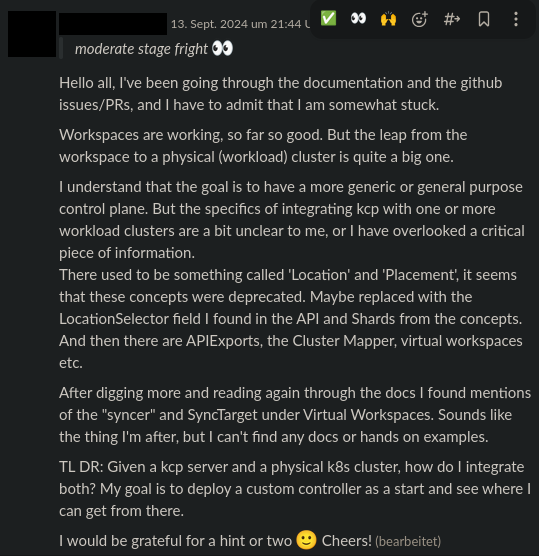
\includegraphics[width=\textwidth]{screenshots/slack/tmc1.anonymized.png}
                    \caption{Thread on TMC (1)}\label{fig:tmc1}
                \end{figure}

                \begin{figure}[h!]
                    \centering
                    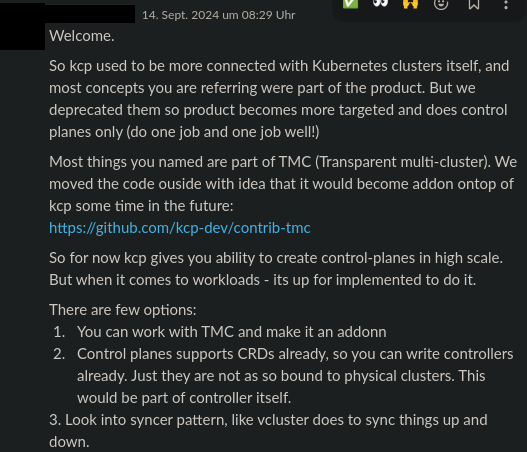
\includegraphics[width=\textwidth]{screenshots/slack/tmc2.anonymized.png}
                    \caption{Thread on TMC (2)}\label{fig:tmc2}
                \end{figure}

                \begin{figure}[h!]
                    \centering
                    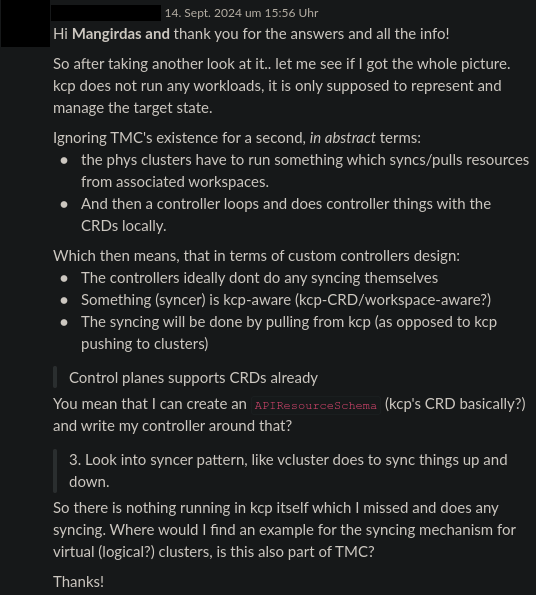
\includegraphics[width=\textwidth]{screenshots/slack/tmc3.anonymized.png}
                    \caption{Thread on TMC (3)}\label{fig:tmc3}
                \end{figure}

                \begin{figure}[h!]
                    \centering
                    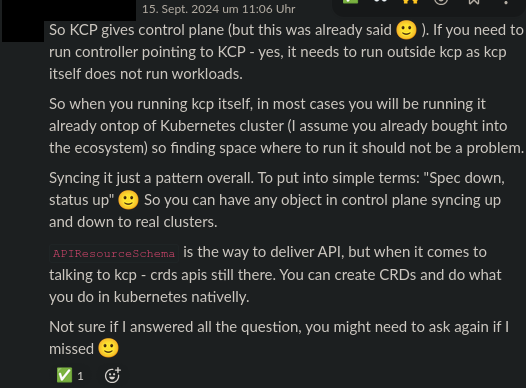
\includegraphics[width=\textwidth]{screenshots/slack/tmc4.anonymized.png}
                    \caption{Thread on TMC (4)}\label{fig:tmc4}
                \end{figure}

                This thread was the rationale for switching to \gls{tmc}.

            \FloatBarrier
            \subsection{Thread on Cross-workspace Resource Reconciliation (2025--08--13)}
                \begin{figure}[h!]
                    \centering
                    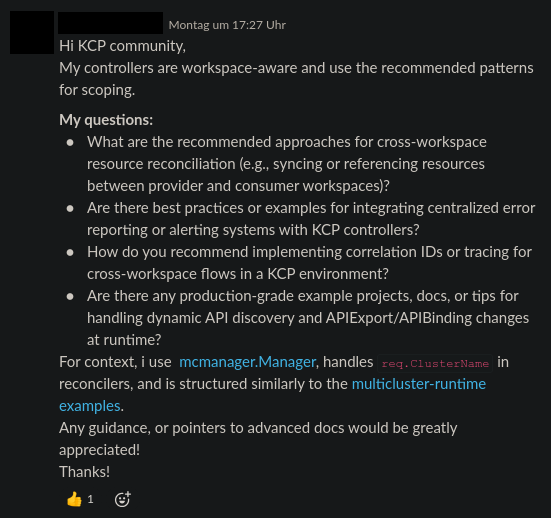
\includegraphics[width=\textwidth]{screenshots/slack/mcr-question.anonymized.png}
                    \caption{MCR related question}\label{fig:mcr-question}
                \end{figure}

                \begin{figure}[h!]
                    \centering
                    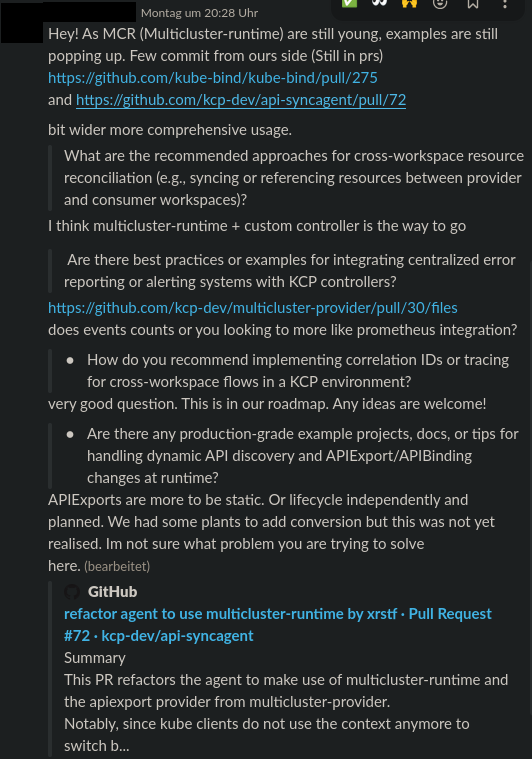
\includegraphics[width=\textwidth]{screenshots/slack/mcr-answer.anonymized.png}
                    \caption{MCR related response}\label{fig:mcr-response}
                \end{figure}

            \FloatBarrier
            \subsection{Thread on Workloads and TMC (2025--04--30)}
                \begin{figure}[h!]
                    \centering
                    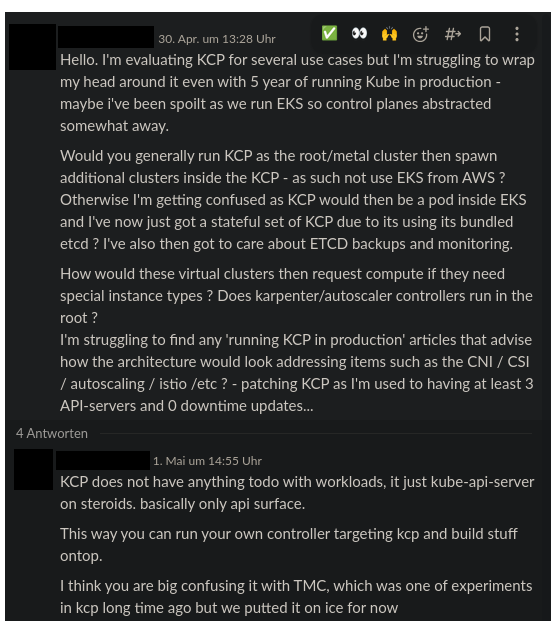
\includegraphics[width=\textwidth]{screenshots/slack/workloads.anonymized.png}
                    \caption{Thread on workloads and TMC}\label{fig:workloads}
                \end{figure}
            
            \FloatBarrier
            \subsection{Thread on api-syncagent (2025--02--13)}
                \begin{figure}[h!]
                    \centering
                    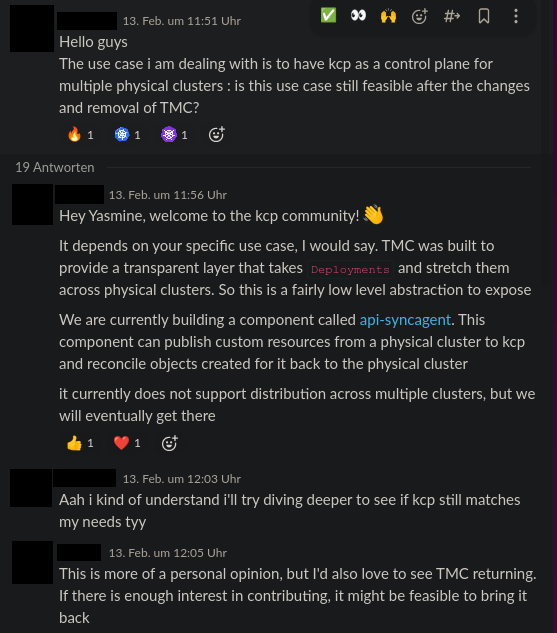
\includegraphics[width=\textwidth]{screenshots/slack/apisyncagent1.anonymized.png}
                    \caption{Thread on api-syncagent (1)}\label{fig:api-syncagent1}
                \end{figure}

                \begin{figure}[h!]
                    \centering
                    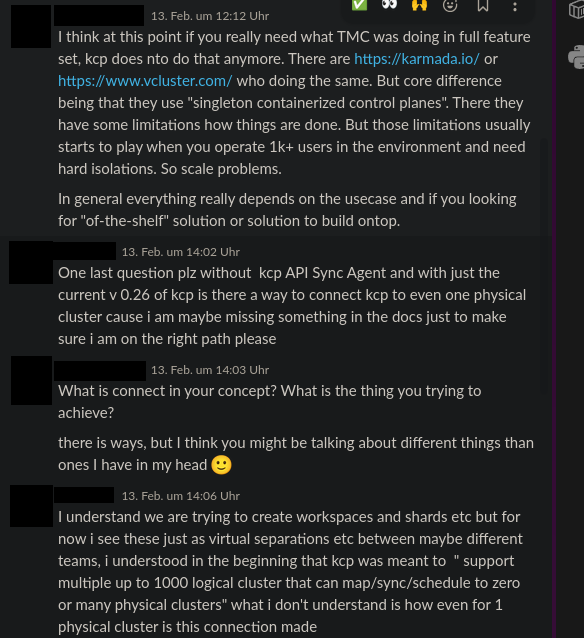
\includegraphics[width=\textwidth]{screenshots/slack/apisyncagent2.anonymized.png}
                    \caption{Thread on api-syncagent (2)}\label{fig:api-syncagent2}
                \end{figure}

                \begin{figure}[h!]
                    \centering
                    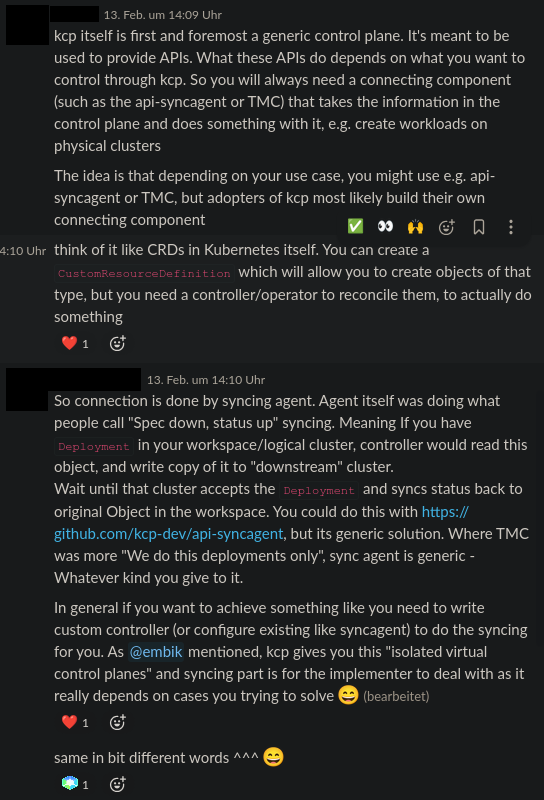
\includegraphics[width=\textwidth]{screenshots/slack/apisyncagent3.anonymized.png}
                    \caption{Thread on api-syncagent (3)}\label{fig:api-syncagent3}
                \end{figure}

            \FloatBarrier
            \subsection{Thread on Removal of TMC (2023--07--21)}
                \begin{figure}[h!]
                    \centering
                    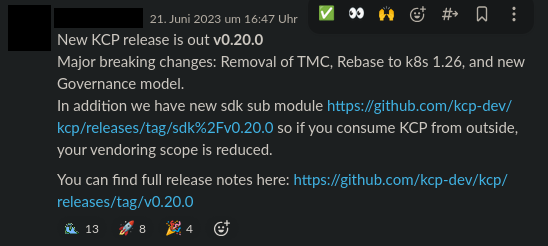
\includegraphics[width=\textwidth]{screenshots/slack/tmc-removal.anonymized.png}
                    \caption{Removal of TMC Announcement}\label{fig:tmc-removal}
                \end{figure}

        \clearpage
        
        % Appendix J: Evaluation
        \section{Evaluation}\label{app:eval}
            \subsection{Dashboard FE}\label{appsub:dashboardfe}
                \begin{figure}[h!]
                    \centering
                    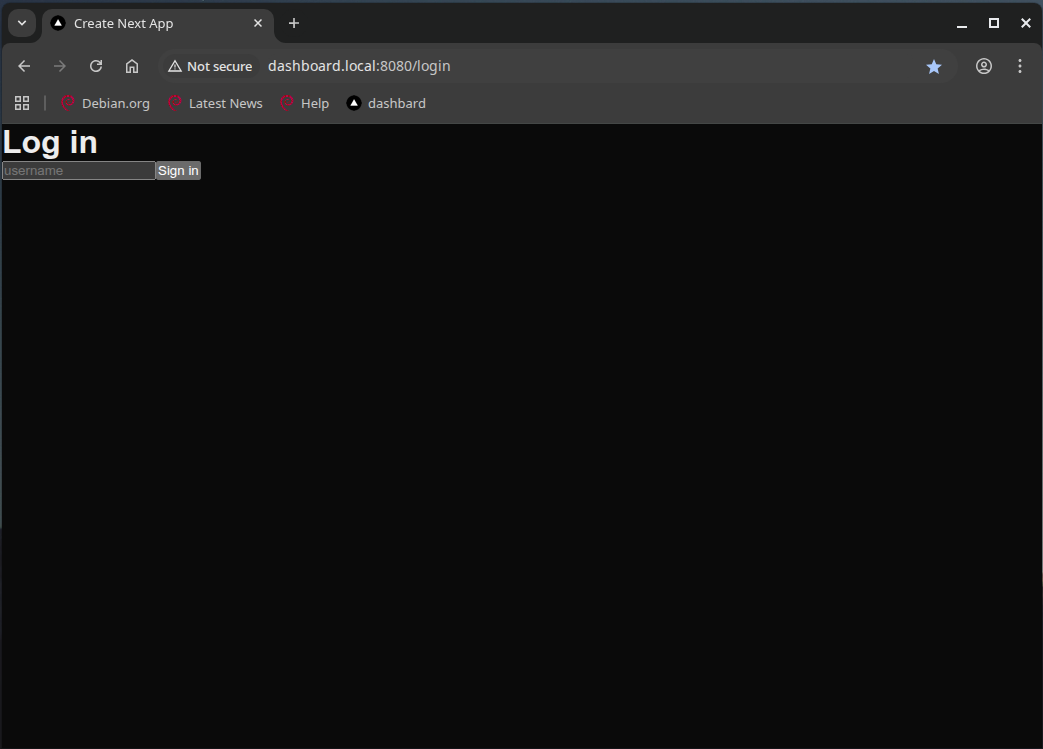
\includegraphics[width=\textwidth]{screenshots/eval/dashboardfe/dashboardfe-login-page.png}
                    \caption{Login page}\label{fig:dashboardfe-login-page}
                \end{figure}

                \begin{figure}[h!]
                    \centering
                    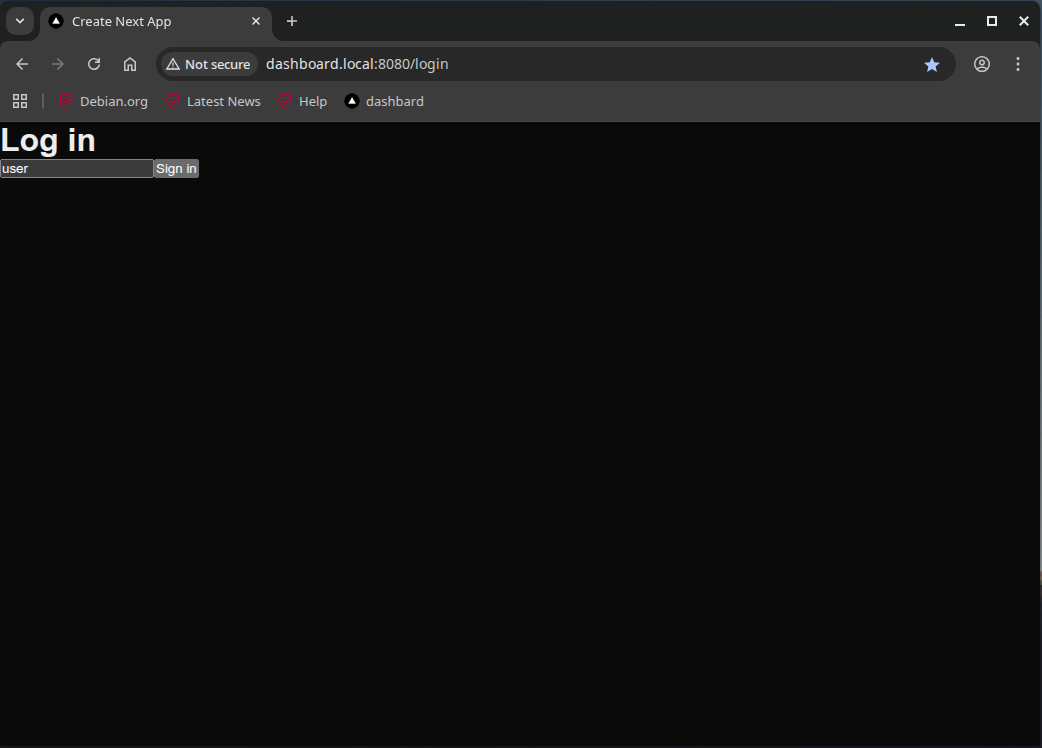
\includegraphics[width=\textwidth]{screenshots/eval/dashboardfe/dashboardfe-login-page-with-username.png}
                    \caption{Login page with username}\label{fig:dashboardfe-login-page-with-username}
                \end{figure}

                \begin{figure}[h!]
                    \centering
                    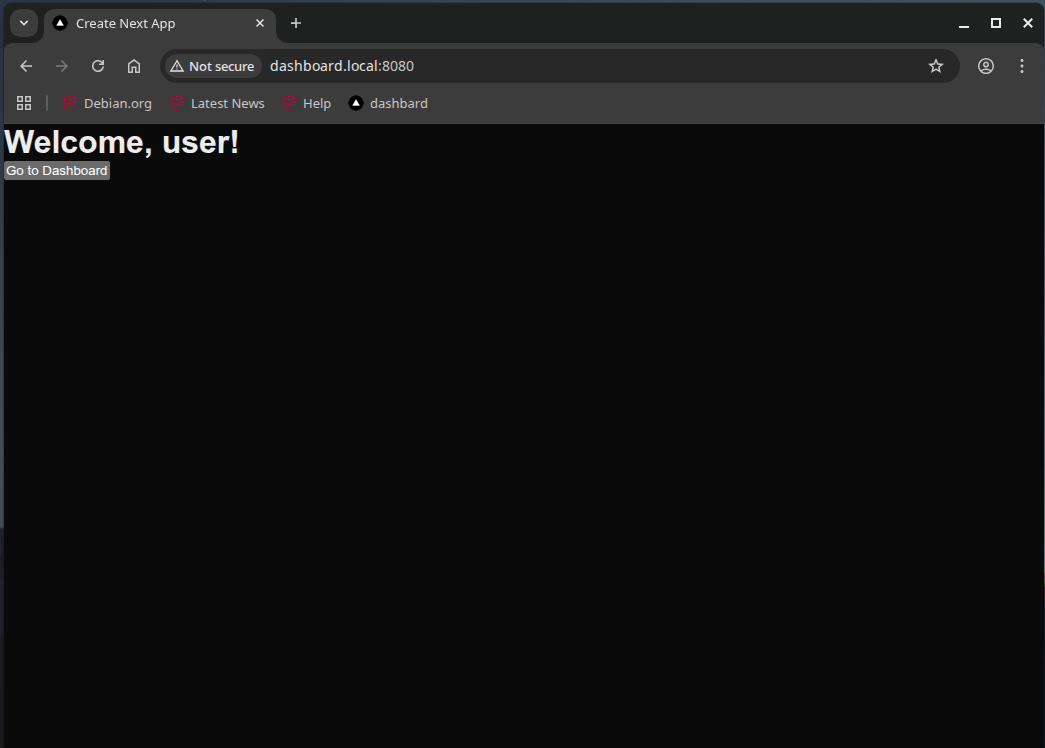
\includegraphics[width=\textwidth]{screenshots/eval/dashboardfe/dashboardfe-welcome-page.png}
                    \caption{Welcome page}\label{fig:dashboardfe-welcome-page}
                \end{figure}

                \begin{figure}[h!]
                    \centering
                    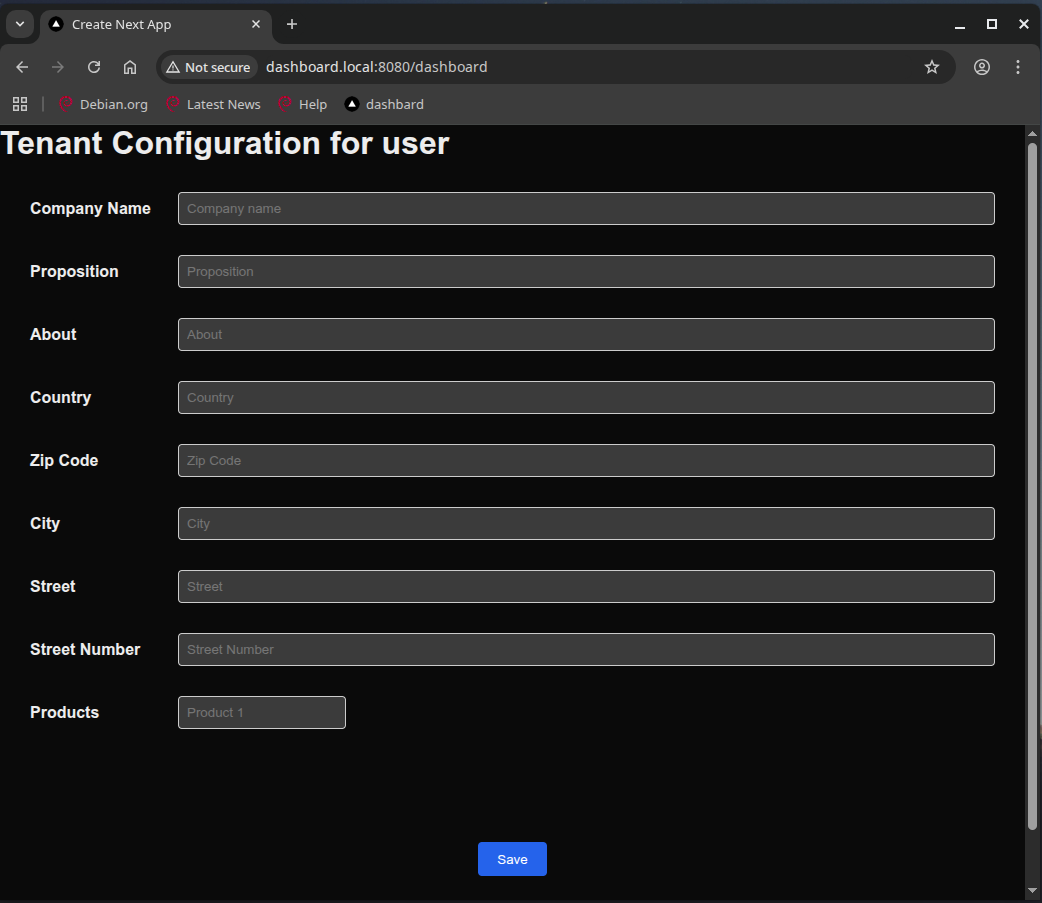
\includegraphics[width=\textwidth]{screenshots/eval/dashboardfe/dashboardfe-form.png}
                    \caption{Form}\label{fig:dashboardfe-form}
                \end{figure}

                \begin{figure}[h!]
                    \centering
                    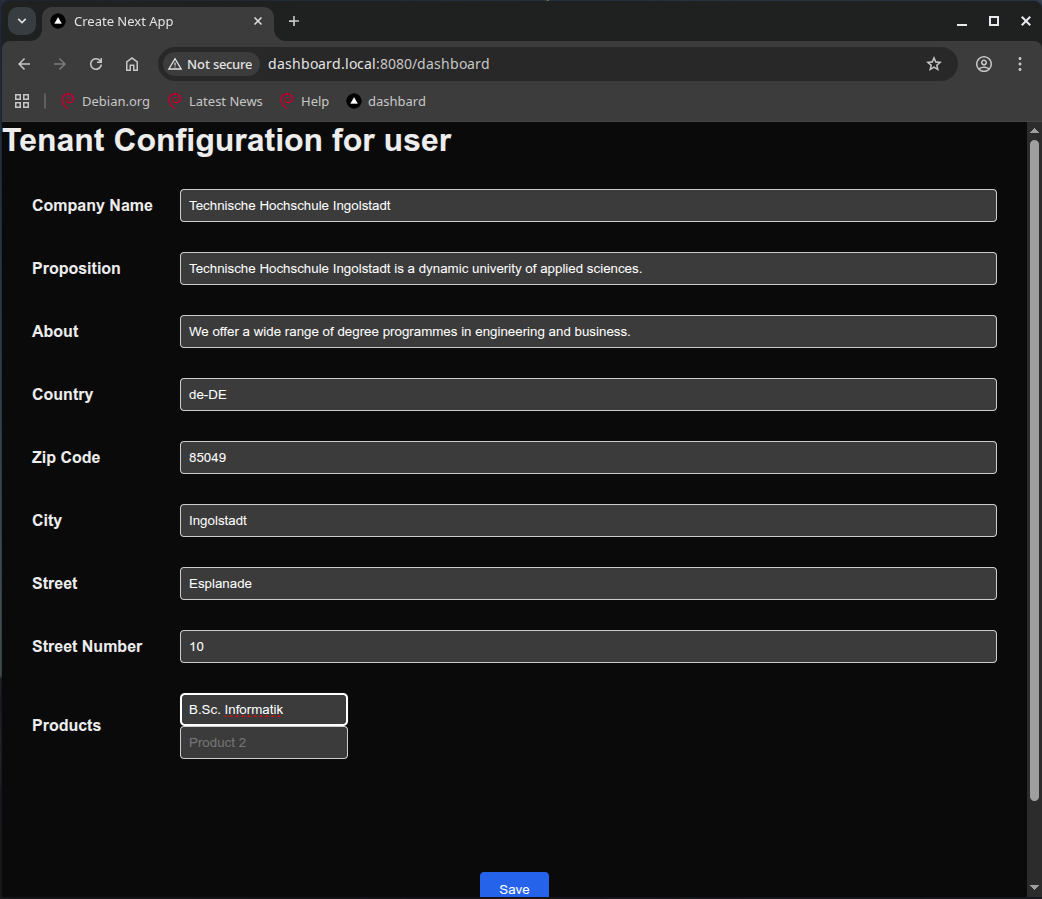
\includegraphics[width=\textwidth]{screenshots/eval/dashboardfe/dashboardfe-form-with-inputs.png}
                    \caption{Form with inputs}\label{fig:dashboardfe-form-with-inputs}
                \end{figure}

                \begin{figure}[h!]
                    \centering
                    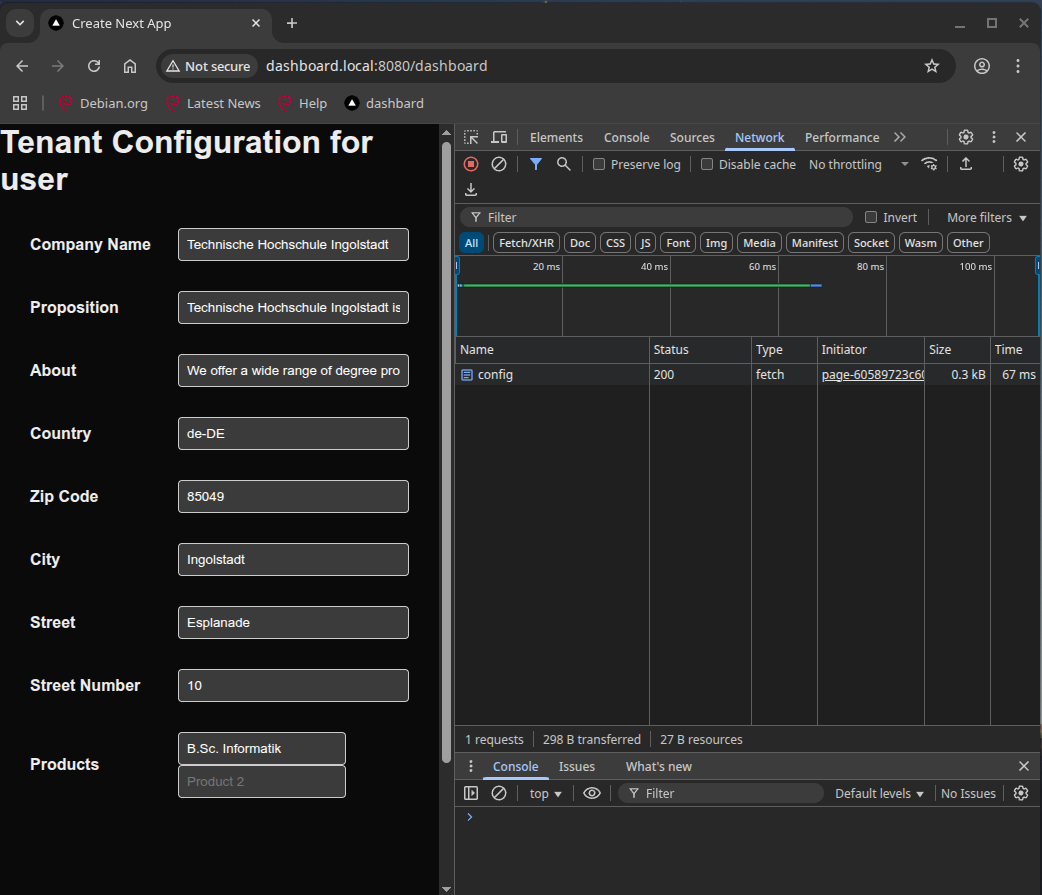
\includegraphics[width=\textwidth]{screenshots/eval/dashboardfe/dashboardfe-form-200.png}
                    \caption{Form-success}\label{fig:dashboardfe-form-200}
                \end{figure}

                \begin{figure}[h!]
                    \centering
                    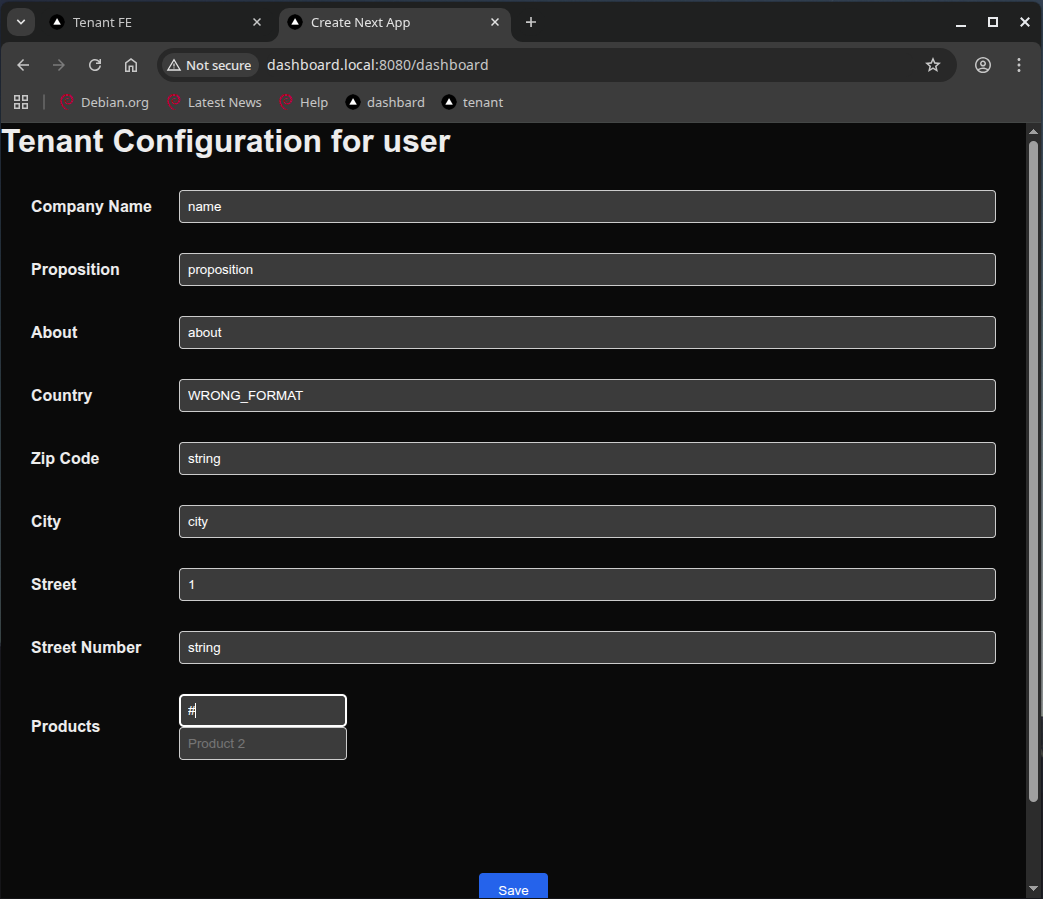
\includegraphics[width=\textwidth]{screenshots/eval/dashboardfe/dashboardfe-form-with-malformed-inputs.png}
                    \caption{Form with malformed inputs}\label{fig:dashboardfe-form-with-malformed-inputs}
                \end{figure}

                \begin{figure}[h!]
                    \centering
                    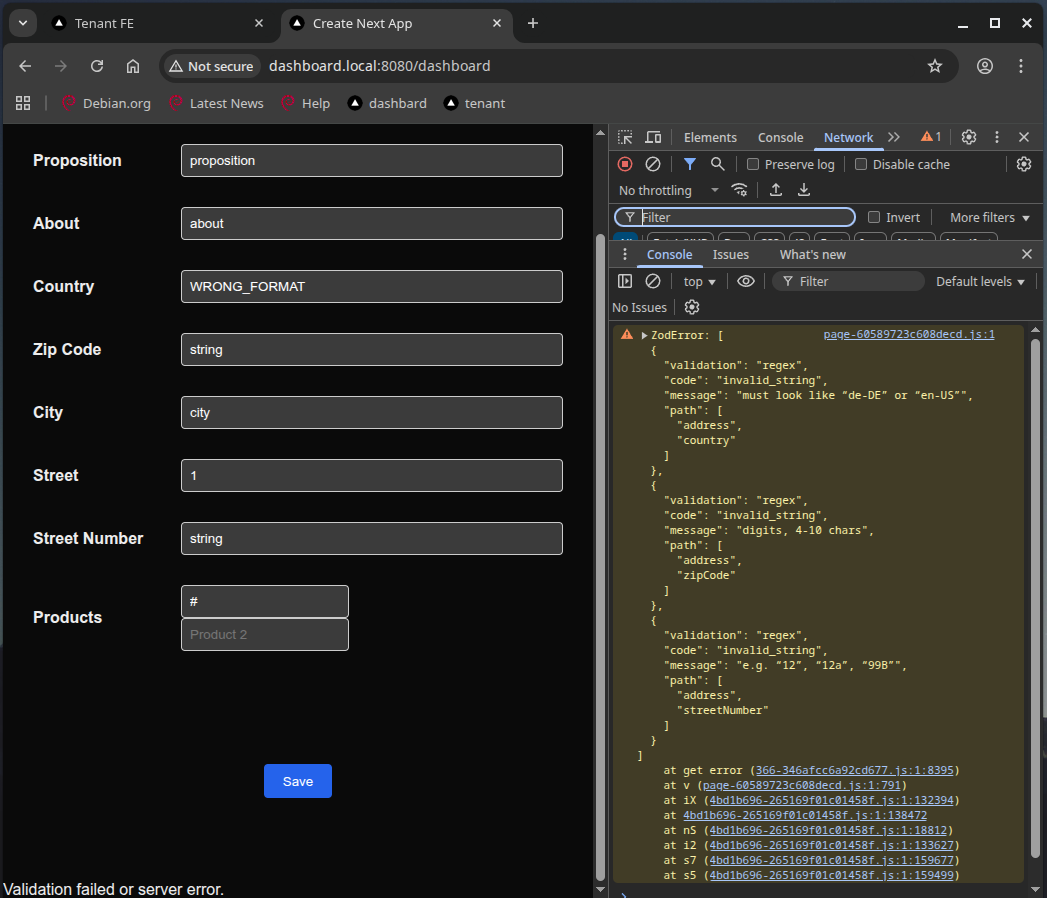
\includegraphics[width=\textwidth]{screenshots/eval/dashboardfe/dashboardfe-validation-failure.png}
                    \caption{Form-validation failure}\label{fig:dashboardfe-form-validation-failure}
                \end{figure}

            \FloatBarrier
            \subsection{Dashboard BE}\label{appsub:dashboardbe}
                \begin{figure}[h!]
                    \centering
                    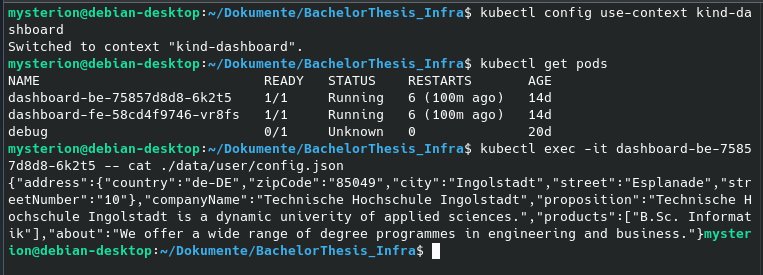
\includegraphics[width=\textwidth]{screenshots/eval/dashboardbe/dashboardbe-config.png}
                    \caption{Config}\label{fig:dashboardbe-config}
                \end{figure}

                \begin{figure}[h!]
                    \centering
                    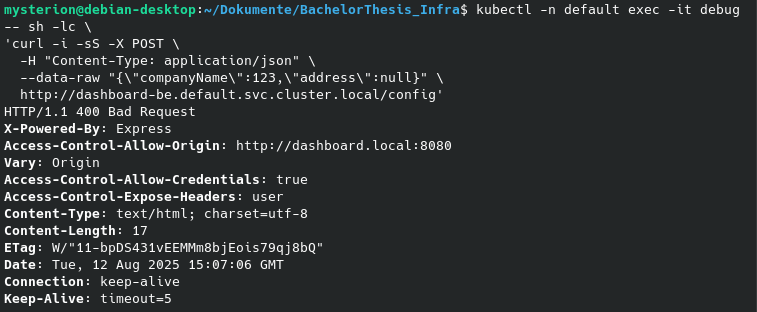
\includegraphics[width=\textwidth]{screenshots/eval/dashboardbe/dashboardbe-bad-request.png}
                    \caption{Dashboard BE Bad Request (curl)}\label{fig:dashboardbe-bad-request}
                \end{figure}

        \clearpage

            \FloatBarrier
            \subsection{Tenant FE}\label{appsub:tenantfe}
                \begin{figure}[h!]
                    \centering
                    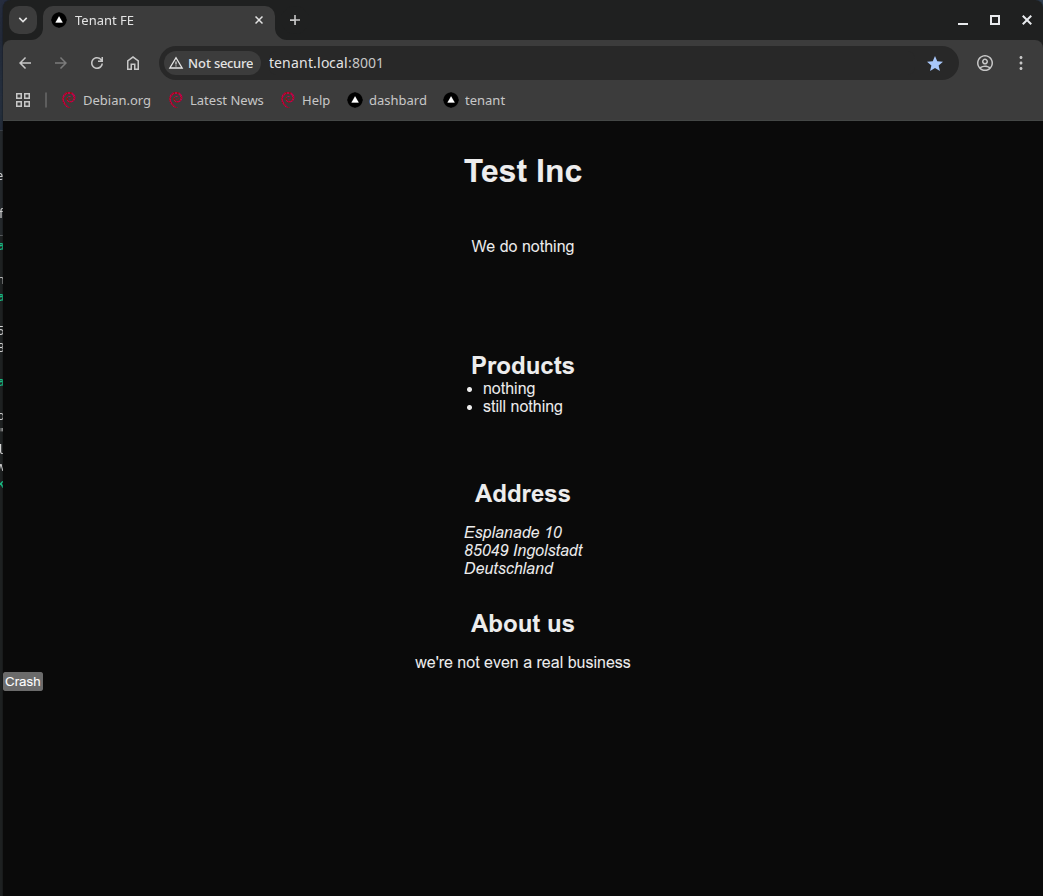
\includegraphics[width=\textwidth]{screenshots/eval/tenantfe/tenantfe.png}
                    \caption{Tenant FE page}\label{fig:tenantfe-page}
                \end{figure}

        \clearpage

            \FloatBarrier
            \subsection{Tenant BE}\label{appsub:tenantbe}
                \begin{figure}[h!]
                    \centering
                    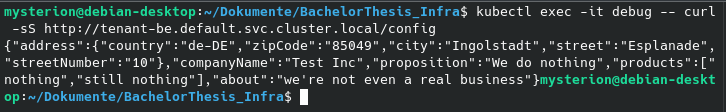
\includegraphics[width=\textwidth]{screenshots/eval/tenantbe/curl.png}
                    \caption{Tenant BE (curl)}\label{fig:tenantbe-curl}
                \end{figure}
                
\end{document}
